\documentclass[12pt,a4paper,oneside]{report}

% -------------------------------------------------
% Paquetes
% -------------------------------------------------
\usepackage[utf8]{inputenc}
\usepackage[T1]{fontenc}
\usepackage[spanish,es-nodecimaldot]{babel}
\usepackage{graphicx}
\graphicspath{{imagenes/}}
\usepackage{booktabs}
\usepackage{tabularx}
\usepackage{array}
\usepackage{ragged2e}
\usepackage{tikz}
\usetikzlibrary{positioning,arrows.meta,fit,shapes.geometric,babel}
\usepackage[table]{xcolor}
\usepackage{geometry}
\usepackage{caption}
\usepackage{float}
\usepackage{pgfgantt}
\usepackage{pdflscape}
\usepackage{afterpage}
\usepackage{pdfpages}
\usepackage{fancyhdr}
\usepackage[hidelinks,pdfpagelayout=SinglePage]{hyperref}
\usepackage{xurl}                      % corta las URL largas de la bibliografía (después de hyperref)
\usepackage{longtable}                 % lista de abreviaturas que continúa en la página siguiente
\setlength{\emergencystretch}{3em}     % evita líneas que se salen del margen

% -------------------------------------------------
% Márgenes y espaciado
% -------------------------------------------------
\geometry{a4paper, left=3cm, right=2.5cm, top=3cm, bottom=3cm}
\linespread{1.5}
\setlength{\parskip}{6pt}
\setlength{\parindent}{0.75cm}

% -------------------------------------------------
% Colores
% -------------------------------------------------
\definecolor{ArduinoTeal}{HTML}{008184}
\definecolor{DeepBlue}{HTML}{16324F}
\definecolor{SoftBlue}{HTML}{EAF2FB}
\definecolor{SoftGreen}{HTML}{E7F6F4}
\definecolor{SoftOrange}{HTML}{FFF3E0}
\definecolor{TableGray}{HTML}{E9EBED}
\definecolor{TableGrayDark}{HTML}{C9CDD2}

% -------------------------------------------------
% Encabezado y pie de página
% -------------------------------------------------
\fancyhf{}
\fancyhead[L]{\small\textcolor{DeepBlue}{Plataforma didáctica PLC, Campus San Carlos}}
\fancyhead[R]{\small María del Milagro Rojas Sánchez}
\fancyfoot[C]{\thepage}
\renewcommand{\headrulewidth}{0.4pt}
% babel-español fija estos nombres al iniciar el documento, por lo que la
% redefinición debe aplicarse después con \AtBeginDocument.
\AtBeginDocument{%
    \renewcommand{\listtablename}{Índice de tablas}%
    \renewcommand{\tablename}{Tabla}%
}

% Color de fila que respeta las lineas verticales de la tabla
\newcommand{\filacolor}[1]{\rowcolor{#1}[\dimexpr\tabcolsep-\arrayrulewidth\relax][\dimexpr\tabcolsep-\arrayrulewidth\relax]}

% Repite la linea horizontal superior de una fila coloreada, dibujandola encima del
% relleno (algunos visores pintan el gris sobre el \hline y la linea desaparece).
% Va al inicio de la primera celda; #1 = ancho total de la tabla
\newcommand{\reglasuperior}[1]{\leavevmode\rlap{\hspace*{-\dimexpr\tabcolsep+\arrayrulewidth\relax}\smash{\raisebox{\arraystretch\ht\strutbox}{\rule{#1}{\arrayrulewidth}}}}}

% Marcador temporal de contenido pendiente
\newcommand{\pendiente}[1]{\textcolor{red}{\textbf{[PENDIENTE: #1]}}}

% Figura exportada desde draw.io: si el PDF aún no está en imagenes/, se
% muestra un recuadro con el nombre esperado en lugar de detener la compilación
\newcommand{\figuraexterna}[2]{\IfFileExists{imagenes/#2}{\includegraphics[#1]{#2}}{\fbox{\parbox{0.8\textwidth}{\centering\small Exportar desde draw.io a \texttt{\detokenize{imagenes/#2}}}}}}

% =================================================================
\begin{document}
% =================================================================

% -------------------------------------------------
% Portada
% -------------------------------------------------
\begin{titlepage}
\thispagestyle{empty}
\centering

{\normalsize Tecnológico de Costa Rica\par}
\vspace{0.1cm}
{\normalsize Escuela de Ingeniería Electrónica\par}
\vspace{0.1cm}
{\normalsize Programa de Licenciatura en Ingeniería Electrónica\par}

\vspace{1.2cm}

\includegraphics[width=90mm]{Logo_TEC.png}

\vspace{1.2cm}

{\LARGE\bfseries\color{DeepBlue}
Diseño de una plataforma didáctica para la enseñanza de PLC
de la Escuela de Ingeniería Electrónica del
Campus Tecnológico Local San Carlos\par}

\vspace{1.8cm}

{\normalsize Informe de proyecto de graduación para optar por el título de\par}
\vspace{0.1cm}
{\normalsize Ingeniería en Electrónica con el grado académico de Licenciatura\par}

\vfill

{\normalsize María del Milagro Rojas Sánchez\par}

\vspace{2.5cm}
{\normalsize San Carlos, noviembre, 2026\par}

\end{titlepage}

% -------------------------------------------------
% Tribunal evaluador (machote del Anexo 2 de la guía del informe final)
% Un solo profesor lector
% -------------------------------------------------
\newcommand{\nombrelector}{Ing. Leonardo Cardinale Villalobos}
\thispagestyle{empty}

\begin{center}
    \textbf{INSTITUTO TECNOLÓGICO DE COSTA RICA}\\[8pt]
    \textbf{ESCUELA DE INGENIERÍA ELECTRÓNICA}\\[8pt]
    \textbf{PROYECTO DE GRADUACIÓN}\\[8pt]
    \textbf{TRIBUNAL EVALUADOR}
\end{center}

\vspace{1.2cm}

\noindent Proyecto de Graduación defendido ante el presente Tribunal Evaluador como
requisito para optar por el título de Ingeniera en Electrónica con el grado académico
de Licenciatura, del Instituto Tecnológico de Costa Rica.

\vspace{0.6cm}

\begin{center}
    Miembros del Tribunal
\end{center}

\vspace{2.2cm}

\noindent
\begin{minipage}[t]{0.49\textwidth}
    \centering
    \rule{6cm}{0.4pt}\\[2pt]
    Ing. Pablo César Rodríguez Vargas\\[6pt]
    Profesor asesor
\end{minipage}
\hfill
\begin{minipage}[t]{0.49\textwidth}
    \centering
    \rule{6cm}{0.4pt}\\[2pt]
    \nombrelector\\[6pt]
    Profesor lector
\end{minipage}

\vspace{2.2cm}

\noindent Los miembros de este Tribunal dan fe de que el presente trabajo de graduación
ha sido aprobado y cumple con las normas establecidas por la Escuela de Ingeniería
Electrónica.

\vspace{1.2cm}

\begin{center}
    San Carlos, noviembre, 2026
\end{center}

\clearpage

% -------------------------------------------------
% Declaratoria de autenticidad (machote del Anexo 3: el texto no puede alterarse)
% -------------------------------------------------
\thispagestyle{empty}

\vspace*{5cm}

\noindent Declaro que el presente Proyecto de Graduación ha sido realizado enteramente por
mi persona, utilizando y aplicando literatura referente al tema e introduciendo
conocimientos propios.

\noindent En los casos en que he utilizado bibliografía, he procedido a indicar las fuentes
mediante las respectivas citas bibliográficas.

\noindent En consecuencia, asumo la responsabilidad total por el trabajo de graduación
realizado y por el contenido del correspondiente informe final.

\vspace{3cm}

\noindent
\begin{minipage}[t]{0.5\textwidth}
    San Carlos, noviembre, 2026
\end{minipage}%
\begin{minipage}[t]{0.5\textwidth}
    % Firma escaneada (fondo eliminado) sobre la línea, sin ocupar espacio vertical
    \rule{6cm}{0.4pt}\llap{\smash{\raisebox{-5mm}{\makebox[6cm]{\IfFileExists{imagenes/Firma_transparente.png}{\includegraphics[height=2.6cm]{Firma_transparente.png}}{}}}}}\\[2pt]
    María del Milagro Rojas Sánchez\\[6pt]
    Céd: 2-0823-0408
\end{minipage}

\clearpage

% -------------------------------------------------
% Resumen
% -------------------------------------------------
\thispagestyle{empty}

\begin{center}
    {\large\bfseries\color{DeepBlue} Resumen}
\end{center}

\vspace{0.5cm}

El programa de Ingeniería Electrónica del Campus Tecnológico Local San Carlos del ITCR
carecía de una plataforma propia para la enseñanza práctica de automatización con PLC.

Se diseñó y construyó una plataforma didáctica modular basada en el Arduino Opta WiFi, el kit
AKX00051 y el módulo analógico AFX00007, montada en un panel de control con riel DIN sobre una
estructura de perfil de aluminio T-slot. Una regleta de borneras identificadas, con cableado
codificado por tipo de señal, permite conectar los dispositivos de campo sin intervenir el
hardware de control, y una tarjeta optoacopladora PC817 permite accionar circuitos propios del
estudiante a la tensión que requieran, entre 3,6 y 30~V. Dos prácticas en Ladder Diagram, documentadas en una
guía de laboratorio, validaron la entrada digital, la salida de relé, la entrada y la salida
analógicas y la salida PWM. El análisis costo-beneficio mostró que un puesto con Siemens
S7-1500 y su licencia cuesta unas 9,5 veces la plataforma, y el equipo base del Festo
EduTrainer unas 11 veces, con funcionalidad comparable para la enseñanza de PLC.

\textbf{Palabras clave:} PLC, automatización industrial, plataforma didáctica, Arduino Opta,
IEC~61131-3, laboratorio de control.

\clearpage

% -------------------------------------------------
% Abstract
% -------------------------------------------------
\thispagestyle{empty}

\begin{center}
    {\large\bfseries\color{DeepBlue} Abstract}
\end{center}

\vspace{0.5cm}

The Electronics Engineering program at Campus Tecnológico Local San Carlos (ITCR) lacked a
dedicated platform for hands-on PLC teaching.

A modular didactic platform based on the Arduino Opta WiFi, the AKX00051 kit, and the AFX00007
analog module was designed and built, mounted on a DIN-rail control panel over a T-slot
aluminum profile frame. A strip of labeled terminals with color-coded wiring lets students
connect field devices without touching the control hardware, and a PC817 optocoupler board
lets them drive their own circuits at whatever voltage they require, from 3.6 to 30~V. Two Ladder Diagram lab
exercises, documented in a student lab guide, validated digital input, relay output, analog
input and output, and PWM output. The cost-benefit analysis showed that a Siemens S7-1500
workstation with its license costs about 9.5 times as much as the platform, and the base Festo
EduTrainer unit about 11 times as much, with comparable functionality for teaching PLC
programming.

\textbf{Keywords:} PLC, industrial automation, didactic platform, Arduino Opta, IEC~61131-3,
control laboratory.

\clearpage

% -------------------------------------------------
% Índice
% -------------------------------------------------
\pagenumbering{roman}
\pagestyle{fancy}
\tableofcontents
\listoffigures
\listoftables

\clearpage

% -------------------------------------------------
% Lista de abreviaturas
% -------------------------------------------------
\section*{Lista de abreviaturas}
\addcontentsline{toc}{section}{Lista de abreviaturas}

\renewcommand{\arraystretch}{1.3}
\begin{longtable}{@{}>{\bfseries}p{2.2cm} p{\dimexpr\textwidth-2.2cm-2\tabcolsep\relax}@{}}
ABS   & Acrilonitrilo butadieno estireno (plástico de impresión 3D) \\
BLE   & \textit{Bluetooth Low Energy} \\
CRC   & Verificación de redundancia cíclica (\textit{Cyclic Redundancy Check}) \\
CTR   & Razón de transferencia de corriente (\textit{Current Transfer Ratio}) \\
DC  & Corriente directa (\textit{Direct Current}) \\
DIN   & \textit{Deutsches Institut für Normung} \\
E/S   & Entradas y salidas \\
FBD   & \textit{Function Block Diagram} (Diagrama de Bloques de Función) \\
IEC   & \textit{International Electrotechnical Commission} \\
IDE   & \textit{Integrated Development Environment} (Entorno de Desarrollo Integrado) \\
ITCR  & Instituto Tecnológico de Costa Rica \\
IVA   & Impuesto al valor agregado \\
LD    & \textit{Ladder Diagram} (Diagrama de Escalera) \\
LED   & Diodo emisor de luz (\textit{Light Emitting Diode}) \\
MDF   & Tablero de fibra de densidad media (\textit{Medium Density Fibreboard}) \\
NA / NC & Normalmente abierto / normalmente cerrado \\
PID   & Controlador proporcional, integral y derivativo \\
PLA   & Ácido poliláctico (plástico de impresión 3D) \\
PLC   & \textit{Programmable Logic Controller} (Controlador Lógico Programable) \\
PVC   & Policloruro de vinilo \\
PWM   & \textit{Pulse Width Modulation} (Modulación por Ancho de Pulso) \\
RS-485 & Estándar de transmisión serie diferencial (\textit{Recommended Standard 485}) \\
RTD   & Detector de temperatura por resistencia (\textit{Resistance Temperature Detector}) \\
RTU   & \textit{Remote Terminal Unit}; en Modbus RTU, transmisión binaria por línea serie \\
SCADA & \textit{Supervisory Control and Data Acquisition} \\
ST    & \textit{Structured Text} (Texto Estructurado) \\
STP / UTP & Par trenzado blindado / sin blindaje (\textit{Shielded / Unshielded Twisted Pair}) \\
TCP   & \textit{Transmission Control Protocol} \\
TEC   & Tecnológico de Costa Rica \\
TFG   & Trabajo Final de Graduación \\
USB   & Bus serie universal (\textit{Universal Serial Bus}) \\
\end{longtable}

\clearpage
\pagenumbering{arabic}

% =================================================================
\chapter{Introducción}
\label{chp:intro}
% =================================================================

La automatización industrial representa uno de los pilares fundamentales de la ingeniería moderna. Los sistemas de control basados en Controladores Lógicos Programables (PLC) se encuentran presentes en prácticamente todos los sectores productivos: manufactura, transporte, energía, gestión de edificios y procesos de servicios, entre otros. En consecuencia, la formación práctica en automatización industrial constituye una competencia esencial para los profesionales de ingeniería eléctrica, electrónica y mecatrónica.

\begin{figure}[H]
    \centering
    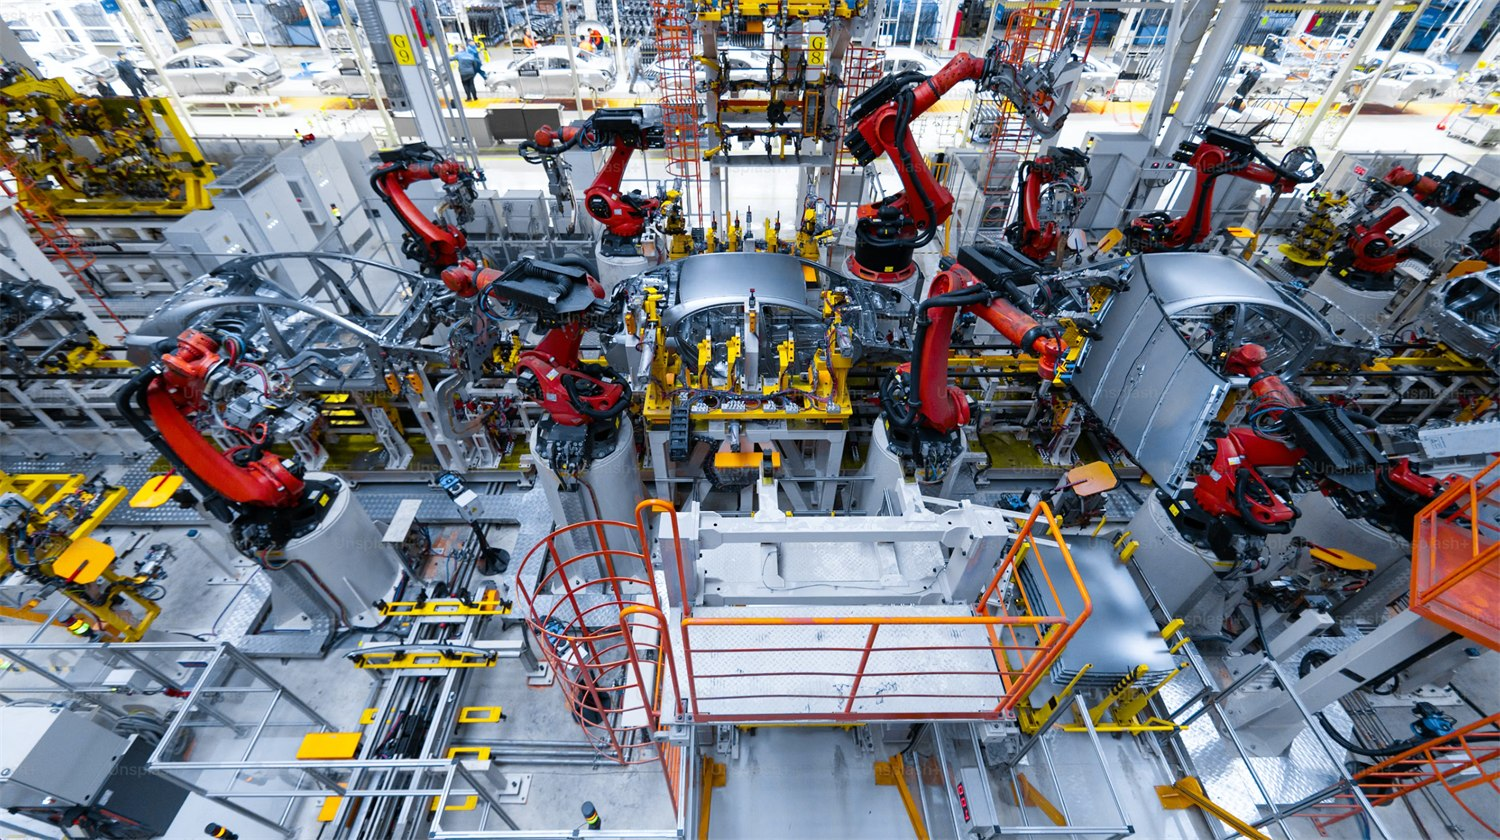
\includegraphics[width=0.9\textwidth]{Vista_aerea_fabrica_red}
    \caption{Planta de ensamblaje de automóviles con brazos robóticos controlados por PLC~\cite{ref9}.}
    \label{fig:fabrica}
\end{figure}

Sin embargo, en la práctica educativa esta formación encuentra obstáculos estructurales: las condiciones que exige un laboratorio de automatización real (en términos de equipamiento, seguridad y adaptabilidad pedagógica) rara vez se encuentran disponibles de manera conjunta en los entornos académicos de ingeniería.

El presente proyecto propone el diseño de una plataforma didáctica modular basada en el Arduino Opta WiFi, un micro-PLC de orientación industrial. El núcleo del sistema es el panel de control, que integra el PLC y sus módulos de expansión sobre una superficie única y rígida y expone terminales de señal accesibles al usuario, permitiendo conectar dispositivos de campo a 24~V~DC de manera segura sin intervenir el hardware principal.

% -------------------------------------------------
\section{Entorno del proyecto}
\label{sec:entorno}
% -------------------------------------------------

Este proyecto se desarrolla dentro del programa de Licenciatura en Ingeniería Electrónica del Campus Tecnológico Local San Carlos del Instituto Tecnológico de Costa Rica (ITCR). El campus prepara ingenieros en áreas como sistemas de control, instrumentación y electrónica industrial, disciplinas directamente relacionadas con la automatización industrial presente en la región Huetar Norte y en el país.

En la carrera, la Escuela de Ingeniería Electrónica ha reconocido la importancia de incorporar los Controladores Lógicos Programables como parte práctica de los cursos. Trabajar con PLC es una habilidad clave para el ingeniero electrónico, ya que implica programar con los lenguajes del estándar IEC 61131-3, conectar señales de campo a 24~V~DC y manejar sensores y actuadores industriales. Sin embargo, actualmente la carrera no cuenta con una plataforma propia para realizar estas prácticas en condiciones similares a las de un entorno industrial real.

Por eso, este proyecto propone diseñar una plataforma didáctica de bajo costo usando el Arduino Opta WiFi como micro-PLC, junto con dispositivos de instrumentación accesibles. La idea es que pueda usarse en distintas materias de la carrera, para que los estudiantes realicen prácticas que conecten los conceptos teóricos con el funcionamiento real de un sistema de control.

\section{Planteamiento del problema}
\label{sec:problema}

\subsection{Estado actual}

La formación práctica en automatización exige que el estudiante programe, cablee, configure entradas y salidas reales, e interprete la respuesta de un sistema físico ante distintas condiciones de control. Estas competencias (programación con lenguajes industriales, conexión de señales a 24 V DC, instrumentación y diagnóstico de fallas) no pueden desarrollarse mediante simulación ni en entornos puramente teóricos; requieren acceso a hardware físico real operando bajo condiciones industriales estándar~\cite{ref3,ref4}.

Sin embargo, la implementación de laboratorios prácticos de automatización enfrenta limitaciones estructurales recurrentes. En primer lugar, los equipos industriales reales implican una inversión económica elevada. Un PLC de gama media con sus módulos de expansión, fuentes de alimentación y accesorios puede representar varios miles de dólares por estación de trabajo~\cite{ref3}, lo que dificulta que las instituciones académicas adquieran y mantengan equipos en cantidad suficiente para cubrir grupos numerosos de estudiantes. En segundo lugar, la mayoría de las plataformas didácticas existentes (tanto los kits comerciales integrados como los montajes propios de laboratorio) están concebidas como sistemas cerrados, de modo que para ejecutar una práctica diferente, el docente o el estudiante debe intervenir directamente sobre el montaje principal, modificando conexiones, recableando terminales o reordenando componentes.

Esta condición genera consecuencias concretas: aumenta el riesgo de errores de conexión, expone el hardware de control a daños por manipulación inadecuada, reduce la flexibilidad para adaptar el sistema a distintos escenarios experimentales y limita la escalabilidad del laboratorio conforme se amplían los contenidos del curso. En la práctica, el tiempo destinado a reconfigurar el sistema compite con el tiempo disponible para el aprendizaje efectivo.

\subsection{Definición del problema}

El programa de Ingeniería Electrónica del Campus San Carlos no dispone actualmente de equipamiento dedicado a la enseñanza de automatización industrial con PLC, ni de un entorno experimental estructurado para desarrollar estas competencias. No obstante, el núcleo del problema no es la ausencia de la plataforma en sí misma (su diseño representará una mejora concreta al estado actual de la carrera), sino la incapacidad operativa que esa carencia genera, pues el programa no puede garantizar hoy que sus estudiantes desarrollen competencias prácticas en automatización industrial de manera segura, técnicamente rigurosa y escalable.

Esta incapacidad se manifiesta en la imposibilidad de realizar prácticas sistemáticas con señales industriales reales a 24~V~DC, de exponer al estudiante a los lenguajes de programación normados por IEC~61131-3 en condiciones de campo, y de adaptar el laboratorio a distintos escenarios experimentales sin comprometer la integridad del hardware de control~\cite{ref3,ref4}.

A lo anterior se suma una desconexión entre los dos ámbitos con los que el estudiante de electrónica trabaja a lo largo de la carrera. La automatización industrial opera a 24~V~DC, mientras que los circuitos que el estudiante diseña y arma en los laboratorios de electrónica funcionan a tensiones menores, típicamente 5~V. Sin una etapa de aislamiento entre ambos niveles de tensión, conectar un circuito propio a las salidas del controlador expone tanto a ese circuito como al hardware de control a daños por diferencia de potencial o por retorno de corriente. En consecuencia, ambos entornos permanecen separados en la formación del estudiante, que no llega a integrarlos en un mismo sistema de control.

\subsection{Síntesis del problema}

El programa de Ingeniería Electrónica del Campus San Carlos carece de un entorno de experimentación adecuado para la enseñanza de automatización industrial con PLC, lo que genera una incapacidad operativa para desarrollar competencias prácticas de manera segura, técnica y escalable con dispositivos de instrumentación de bajo costo.

% -------------------------------------------------
\section{Alcances}
\label{sec:alcances}
% -------------------------------------------------

El presente proyecto abarca el diseño completo de la plataforma didáctica y su verificación
experimental con dispositivos de instrumentación de bajo costo, en el ámbito del programa de
Ingeniería Electrónica del Campus Tecnológico Local San Carlos del ITCR. Los alcances
específicos son los siguientes:

\begin{itemize}
    \item \textbf{Diseño del panel de control:} selección, dimensionamiento y disposición de los
    componentes en riel DIN; diseño del esquema de cableado interno con código de colores por tipo
    de señal; identificación de borneras; y montaje físico de la plataforma con su sistema de
    alimentación a 24~V~DC.

    \item \textbf{Integración del hardware:} configuración del Arduino Opta WiFi con los módulos
    DIN Simul8, DIN Celsius y el módulo analógico AFX00007, cubriendo señales digitales
    (0/24~V~DC), analógicas (0--10~V, 4--20~mA y PT100) y salidas PWM.

    \item \textbf{Interfaz de aislamiento para circuitos de baja tensión:} incorporación a la
    plataforma de una tarjeta optoacopladora PC817 de cuatro canales que permite accionar desde
    el controlador circuitos electrónicos construidos por el estudiante, alimentados con su propia
    fuente a la tensión que requieran (de 3,6 a 30~V, habitualmente 5~V), sin contacto eléctrico entre el lado industrial y el lado electrónico~\cite{ref13}.

    \item \textbf{Verificación experimental:} pruebas funcionales con al menos un dispositivo de
    campo por tipo de señal soportada, con resultados documentados, y elaboración de una guía de
    práctica de laboratorio estructurada.

    \item \textbf{Análisis de costo-beneficio:} comparación técnica y económica entre la
    plataforma propuesta y sistemas PLC industriales convencionales de capacidades equivalentes,
    con precios de referencia documentados.

    \item \textbf{Programación:} implementación de lógicas de control de demostración en Ladder
    Diagram (LD), el lenguaje IEC~61131-3 más extendido en la industria, suficientes para la
    validación funcional de la plataforma. Los demás lenguajes soportados por el Arduino PLC IDE
    (FBD y ST) se introducen mediante los tutoriales oficiales que enlaza la guía de laboratorio.
\end{itemize}

% -------------------------------------------------
\section{Limitaciones}
\label{sec:limitaciones}
% -------------------------------------------------

El proyecto está sujeto a las siguientes limitaciones, que delimitan su alcance y contextualizan
sus resultados:

\begin{itemize}
    \item \textbf{Escala de producción:} el diseño corresponde a una unidad prototipo. No
    contempla la fabricación en serie ni la normalización de un proceso de manufactura para
    múltiples unidades.

    \item \textbf{Protocolos de comunicación industrial:} la plataforma no incluye la
    implementación física ni prácticas de laboratorio con protocolos industriales de red. La
    capacidad del Arduino Opta para comunicarse mediante Modbus RTU (sobre su interfaz RS-485) y
    Modbus TCP (sobre Ethernet) se documenta en la sección~\ref{subsec:modbus} como base para la
    proyección futura de la plataforma, pero no se cablea ni se valida experimentalmente en este
    proyecto. Otros protocolos como PROFIBUS, EtherNet/IP u OPC-UA quedan fuera del alcance.

    \item \textbf{Programación avanzada:} las prácticas de verificación se limitan a lógicas de
    control básicas. El desarrollo de aplicaciones de control avanzado (PID multi-lazo, control de
    movimiento, sistemas SCADA) excede el alcance de este proyecto.

    \item \textbf{Disponibilidad de componentes:} los precios y la disponibilidad del hardware
    Arduino están sujetos a variaciones de mercado y de tipo de cambio al momento de la
    adquisición. El presupuesto presentado utiliza precios de referencia vigentes al primer
    semestre de 2026.

    \item \textbf{Validación pedagógica formal:} el proyecto no incluye un estudio controlado sobre
    el impacto en el aprendizaje de los estudiantes. La verificación de la plataforma se limita a
    pruebas funcionales de ingeniería.

    \item \textbf{Carcasa exterior cerrada:} el diseño se concentra en la estructura de soporte,
    en el panel de control con riel DIN y en el sistema de cableado. El diseño de una carcasa
    exterior cerrada con paneles, bisagras o cierre queda fuera del alcance de este proyecto.
\end{itemize}

% -------------------------------------------------
\section{Estructura del documento}
\label{sec:estructura}
% -------------------------------------------------

La sección~\ref{sec:entorno} describe el entorno institucional y curricular que da origen a la
iniciativa. La sección~\ref{sec:problema} expone el planteamiento del problema, incluyendo el
estado actual de los laboratorios de automatización y la definición formal del problema de diseño.
La sección~\ref{sec:alcances} define los alcances del proyecto y la sección~\ref{sec:limitaciones}
establece sus limitaciones. El capítulo~\ref{chp:metaobj} presenta la meta del proyecto y los
objetivos general y específicos, cada uno con su indicador de cumplimiento. El capítulo~\ref{chp:marco}
presenta el marco teórico que sustenta el diseño: los fundamentos de los sistemas PLC, las señales
industriales estándar, el estándar IEC~61131-3 y el Arduino Opta como base tecnológica del proyecto, incluidas sus
capacidades de comunicación industrial mediante RS-485 y Modbus;
e incluye el estado del arte en plataformas didácticas de automatización industrial con el
posicionamiento del proyecto en relación con los enfoques documentados en la literatura. El
capítulo~\ref{chp:procedimientos} describe el procedimiento metodológico seguido para la ejecución
del proyecto, organizado según las fases del método de diseño en ingeniería: el reconocimiento y la
definición del problema, la obtención y el análisis de la información técnica, la evaluación de las
alternativas y la síntesis de una solución mediante matrices de Pugh, la implementación de la
estructura de soporte y su reevaluación. El capítulo~\ref{chp:enfoque} describe la solución
propuesta en detalle: el análisis de soluciones y la selección final, la descripción del hardware
y del software de la plataforma, y el análisis costo-beneficio frente a los PLC industriales convencionales. El capítulo~\ref{chp:resultados} presenta los resultados de las prácticas de verificación y los analiza frente a los objetivos, y el capítulo~\ref{chp:conclusiones} reúne las conclusiones y las recomendaciones para reproducir la plataforma.

% =================================================================
\chapter{Meta y Objetivos}
\label{chp:metaobj}
% =================================================================

Este capítulo presenta la meta del proyecto, que expresa el beneficio que se espera para el Campus, y los objetivos general y específicos que la concretan. Cada uno se acompaña de los indicadores con que se verifica su cumplimiento en el Capítulo~\ref{chp:resultados}.

% -------------------------------------------------
\section{Meta}
% -------------------------------------------------

Lograr que los estudiantes y docentes del Campus Tecnológico Local San Carlos cuenten con un recurso experimental funcional para la enseñanza y aprendizaje de automatización industrial con PLC, superando la carencia de infraestructura dedicada que actualmente limita el desarrollo de estas competencias en el programa.

\textbf{Indicador:} la plataforma diseñada queda lista, junto con su guía de laboratorio, para utilizarse en actividades académicas con estudiantes del Campus Tecnológico Local San Carlos.

% -------------------------------------------------
\section{Objetivos}
% -------------------------------------------------

\subsection{Objetivo general}

Diseñar una plataforma didáctica modular para la enseñanza de PLC, utilizando la tecnología Arduino Opta y dispositivos de instrumentación de bajo costo, que garantice la integridad eléctrica del sistema y permita el desarrollo de competencias prácticas en automatización industrial en el programa de Ingeniería Electrónica del Campus Tecnológico Local San Carlos del ITCR.

Indicador: plataforma funcional que permita ejecutar al menos una práctica completa de programación PLC con lenguajes IEC~61131-3 y conexión de señales industriales a 24~V~DC.

\subsection{Objetivos específicos}

\begin{enumerate}

    \item Diseñar el panel de control que integre el PLC y sus módulos de expansión, exponiendo terminales de señal accesibles que permitan la conexión segura de dispositivos de campo a 24~V~DC.
    \begin{itemize}
        \item Indicador 1: panel de control con el Arduino Opta y sus módulos de expansión montados en riel DIN, organizados siguiendo un flujo ordenado de conexiones que refleje la secuencia lógica de entradas y salidas del sistema.
        \item Indicador 2: entradas y salidas de señal (digitales, analógicas y PWM) identificadas mediante un código de colores distintivo por tipo de señal, con cableado interno visible acorde a dicho código, etiquetado completo y verificación de continuidad en todas las conexiones.
        \item Indicador 3: terminales de alimentación y tierra ubicadas en una zona físicamente separada de las terminales de señal, con código de colores propio y etiquetado que las identifica de forma inequívoca, eliminando el riesgo de confusión durante la conexión.
    \end{itemize}

    \item Verificar el funcionamiento de la plataforma mediante experimentos que demuestren la adquisición de señales de campo y la ejecución de lógica de control programada.
    \begin{itemize}
        \item Indicador 1: elaboración de una guía de práctica de laboratorio estructurada que permita al estudiante programar, cablear y validar una lógica de control básica utilizando plataformas físicas y virtuales.
        \item Indicador 2: validación funcional de cada tipo de señal (digital, analógica y PWM) mediante pruebas con al menos un dispositivo de instrumentación de bajo costo por tipo, con los resultados documentados.
    \end{itemize}

    \item Comparar el costo beneficio de la plataforma propuesta frente a soluciones equivalentes de PLC industriales convencionales.
    \begin{itemize}
        \item Indicador 1: tabla comparativa de costos de hardware y licencias de software entre la plataforma propuesta y sistemas PLC industriales convencionales (Siemens, Festo y/o Allen-Bradley), con precios de referencia documentados.
        \item Indicador 2: análisis de características técnicas equivalentes (lenguajes IEC~61131-3, capacidad de entradas/salidas, conectividad) que respalde la comparabilidad funcional entre los sistemas evaluados.
    \end{itemize}

\end{enumerate}

% =================================================================
\chapter{Marco teórico}
\label{chp:marco}
% =================================================================

Este capítulo reúne los fundamentos técnicos en que se apoya el diseño de la plataforma: el funcionamiento de los PLC; las señales industriales que manejan y el aislamiento galvánico necesario para acoplarlas con circuitos de baja tensión; los lenguajes de la norma IEC~61131-3; las características del Arduino Opta y sus capacidades de comunicación; el estado del arte en plataformas didácticas de automatización y, por último, las herramientas FluidSIM y EasyPort con que se amplían las prácticas.

\section{Controladores Lógicos Programables (PLC)}

Un Controlador Lógico Programable (PLC, del inglés \textit{Programmable Logic Controller}) es un dispositivo electrónico industrial diseñado para automatizar procesos discretos y continuos mediante la lectura de señales de entrada, la ejecución de una lógica de control programada y la activación de señales de salida~\cite{ref3}. A diferencia de los sistemas de control basados en relés o circuitos discretos cableados, el PLC permite modificar la lógica de control mediante software sin alterar el cableado del sistema, lo que le confiere una gran flexibilidad operativa.

\begin{figure}[H]
    \centering
    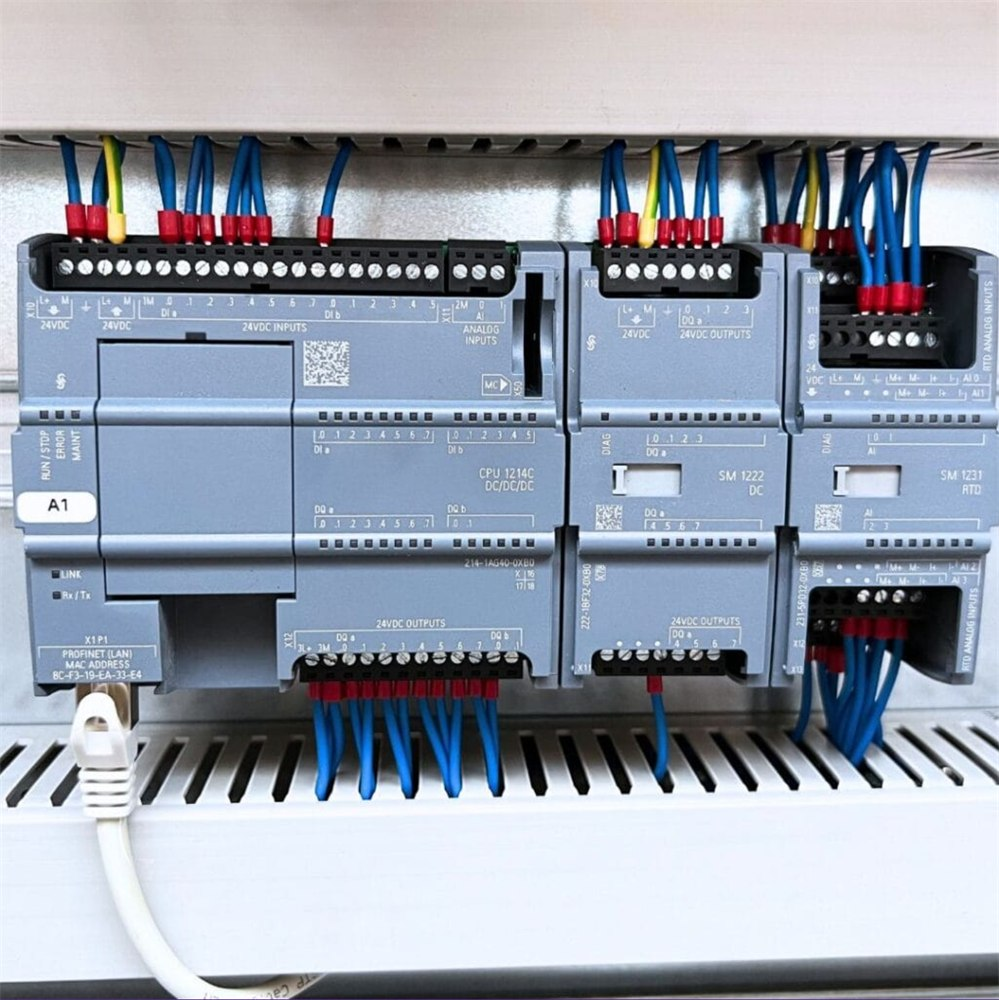
\includegraphics[width=0.8\textwidth]{PLC_industrial_Siemens_red}
    \caption{PLC industrial Siemens SIMATIC S7-1200~\cite{ref7}.}
    \label{fig:plc_siemens}
\end{figure}

\subsection{Ciclo de operación}

El funcionamiento de un PLC se basa en un ciclo de ejecución secuencial continuo, denominado \textit{scan cycle}, que comprende tres etapas fundamentales:

\begin{enumerate}
    \item \textbf{Lectura de entradas:} el PLC lee el estado de todas sus entradas digitales y analógicas y actualiza la imagen de proceso de entradas en memoria.
    \item \textbf{Ejecución del programa:} se ejecuta la lógica de control programada utilizando los valores leídos, calculando el estado que deben tener las salidas.
    \item \textbf{Actualización de salidas:} los valores calculados se transfieren a las salidas físicas del equipo, activando o desactivando los actuadores conectados.
\end{enumerate}

Este ciclo se repite continuamente, con tiempos de scan típicos del orden de los milisegundos, lo que garantiza una respuesta en tiempo real adecuada para la mayoría de las aplicaciones industriales.

\subsection{Características y aplicaciones}

Los PLC destacan por su robustez frente a condiciones industriales adversas (vibraciones, temperatura, humedad e interferencias electromagnéticas), su facilidad de mantenimiento, su escalabilidad mediante módulos de expansión y su alta disponibilidad. Son ampliamente utilizados en sistemas de transporte y clasificación de materiales, líneas de envasado, control de motores eléctricos, instrumentación de procesos y sistemas de supervisión SCADA~\cite{ref3}.

\section{Señales industriales}

En los sistemas de automatización industrial, las señales que intercambian el PLC y los elementos de campo se clasifican en señales digitales y señales analógicas.

\subsection{Señales digitales}

Las entradas digitales detectan eventos discretos (presencia de un objeto, posición de un actuador, activación de un pulsador) mediante sensores de dos estados: activo o inactivo. En entornos industriales estándar, el nivel lógico activo corresponde a 24 V DC. Los sensores pueden ser de tipo NPN (sinking, colector abierto a GND) o PNP (sourcing, colector abierto a +24 V).

Las salidas digitales conmutan cargas externas y pueden ser transistorizadas (NPN o PNP) o de tipo relé. Las salidas de relé, como las del Arduino Opta, proporcionan un contacto seco (libre de tensión) que permite conmutar circuitos de corriente alterna o continua con una capacidad típica de hasta 250 VAC / 5 A, sin que el PLC alimente directamente la carga.

\subsection{Señales analógicas}

Las entradas analógicas permiten adquirir variables físicas continuas (temperatura, presión, caudal, nivel) mediante transductores que convierten la magnitud física en una señal eléctrica estándar. Los rangos más comunes en la industria son:

\begin{itemize}
    \item \textbf{0--10 V DC:} señal de tensión, sencilla de cablear pero susceptible a caídas de tensión en distancias largas.
    \item \textbf{4--20 mA:} señal de corriente, preferida en entornos industriales por su inmunidad al ruido eléctrico y la posibilidad de detectar falla de lazo (0 mA indica cable roto o sensor sin alimentación).
    \item \textbf{PT100 / PT1000:} resistencias de platino para medición de temperatura, con variación lineal de resistencia en función de la temperatura.
    \item \textbf{Termopar tipo K/J/T:} sensores de temperatura de amplio rango (hasta 850°C para tipo K), basados en el efecto Seebeck.
\end{itemize}

Las salidas analógicas permiten gobernar dispositivos de control proporcional (variadores de frecuencia, válvulas modulantes, actuadores lineales) mediante señales de 0--10 V o 4--20 mA generadas por el PLC.

\subsection{Aislamiento galvánico y acoplamiento óptico}
\label{subsec:optoacoplador}

Las señales descritas hasta aquí pertenecen al dominio industrial de 24~V~DC, mientras que los circuitos electrónicos de propósito general operan con tensiones menores, que dependen de cada diseño; la más habitual en los laboratorios de electrónica es 5~V, aunque también son frecuentes alimentaciones de 9 o 12~V. Interconectar ambos dominios de forma directa obliga a compartir la referencia de tierra, de modo que una sobretensión, una inversión de polaridad o un cortocircuito originado en el circuito de baja tensión encuentra un camino conductivo hacia el controlador. El aislamiento galvánico evita esa situación, ya que transmite la información entre dos circuitos sin que exista continuidad eléctrica entre ellos, de manera que cada lado conserva su propia fuente de alimentación y su propia referencia de tierra.

El optoacoplador es el dispositivo más difundido para conseguirlo en el nivel de señal. Encapsula un diodo emisor de infrarrojo y un fototransistor enfrentados ópticamente y separados por una barrera dieléctrica. Cuando circula corriente por el diodo, la radiación emitida incide sobre la región de base del fototransistor y lo lleva a conducción; al cesar la corriente de entrada, el fototransistor vuelve al corte. Lo que atraviesa la barrera es luz y no corriente, por lo que la entrada y la salida quedan eléctricamente independientes.

Tres parámetros gobiernan su aplicación. La tensión de aislamiento indica la diferencia de potencial que la barrera soporta entre la entrada y la salida, y expresa hasta qué punto ambos dominios quedan efectivamente independientes. La razón de transferencia de corriente (CTR) relaciona la corriente de salida del fototransistor con la corriente de entrada del diodo, y determina el valor de la resistencia limitadora necesaria para garantizar la conmutación completa del dispositivo. Por último, los rangos de tensión admisibles en cada lado definen con qué niveles lógicos puede trabajar el componente en la entrada y en la salida, y son los que establecen si un dispositivo dado puede acoplar directamente dos dominios determinados sin electrónica intermedia. Como el lado de salida se alimenta desde el circuito acoplado, un rango de salida amplio permite que ese circuito trabaje con la tensión que su propio diseño requiera, sin cambiar el dispositivo. Como referencia, una tarjeta comercial de cuatro canales basada en el optoacoplador PC817 admite en la entrada señales de 3,6 a 24~V y opera en la salida con tensiones de 3,6 a 30~V~\cite{ref13}, de modo que acepta directamente el nivel de 24~V~DC de un PLC y, del otro lado, cualquier alimentación habitual de un circuito electrónico, de 5~V en adelante.

El contacto seco de un relé, descrito en el apartado de señales digitales, proporciona igualmente separación galvánica, pero se trata de un elemento electromecánico, por lo que su velocidad de conmutación es baja, sus contactos presentan rebote y su vida útil es finita. El acoplamiento óptico, en cambio, conmuta en el orden de los microsegundos, no sufre desgaste mecánico y no introduce rebote, lo que lo hace preferible cuando el elemento gobernado es un circuito electrónico y no una carga de potencia. Ambos mecanismos resultan por tanto complementarios y atienden niveles distintos del sistema.

Una plataforma didáctica que aspire a integrar el control industrial con la electrónica de baja tensión que el estudiante construye en los demás laboratorios de la carrera requiere, por tanto, una etapa de acoplamiento de esta naturaleza. Sin ella ambos ámbitos permanecen como prácticas separadas, ya que el dominio de 24~V~DC no puede gobernar circuitos de baja tensión sin comprometer el hardware de control, y el alcance de lo que el estudiante puede diseñar queda acotado de antemano a los dispositivos de campo previstos. La incorporación de un optoacoplador es lo que permite que ambos mundos se combinen en un mismo sistema y que el diseño propio del estudiante no encuentre en la plataforma un límite. Las alternativas comerciales disponibles se evalúan en el Capítulo~\ref{chp:procedimientos} y la selección del dispositivo concreto se presenta en la Sección~\ref{subsec:seleccion_opto}.

\section{Estándar IEC 61131-3}
\label{sec:iec}

La norma IEC 61131-3 establece los lenguajes de programación estándar para PLC industriales~\cite{ref4}. Su objetivo es garantizar la portabilidad y legibilidad del software de control entre diferentes fabricantes y plataformas. La norma define cinco lenguajes; los tres más utilizados en entornos educativos, y directamente compatibles con el Arduino Opta mediante el PLC IDE de Arduino, son Ladder Diagram (LD), Function Block Diagram (FBD) y Structured Text (ST).

\subsection{Ladder Diagram (LD)}

El Ladder Diagram (o Diagrama de Escalera) es el lenguaje más extendido históricamente. Su notación gráfica imita los esquemas de circuitos de relés eléctricos: contactos normalmente abiertos (NA) y normalmente cerrados (NC) representan condiciones lógicas de entrada, mientras que bobinas representan las salidas activadas. Es intuitivo para técnicos y profesionales con formación en electricidad industrial.

\subsection{Function Block Diagram (FBD)}

El FBD representa la lógica de control mediante bloques funcionales interconectados (compuertas lógicas, temporizadores, contadores, controladores PID). La información fluye de izquierda a derecha a través de las conexiones entre bloques. Es especialmente adecuado para procesos continuos y control de lazos de regulación.

\subsection{Structured Text (ST)}

El Structured Text es un lenguaje de alto nivel con sintaxis similar a Pascal o C. Permite implementar algoritmos complejos, estructuras de control (IF-THEN-ELSE, FOR, WHILE, CASE) y operaciones matemáticas de forma concisa y legible para programadores con formación en software.

\vspace{0.4cm}

La figura~\ref{fig:iec61131} ilustra un mismo programa de control (activar la salida O1 cuando se cumplen simultáneamente las condiciones de entrada I1 e I2) expresado en los tres lenguajes definidos por IEC 61131-3.

\begin{figure}[H]
    \centering
    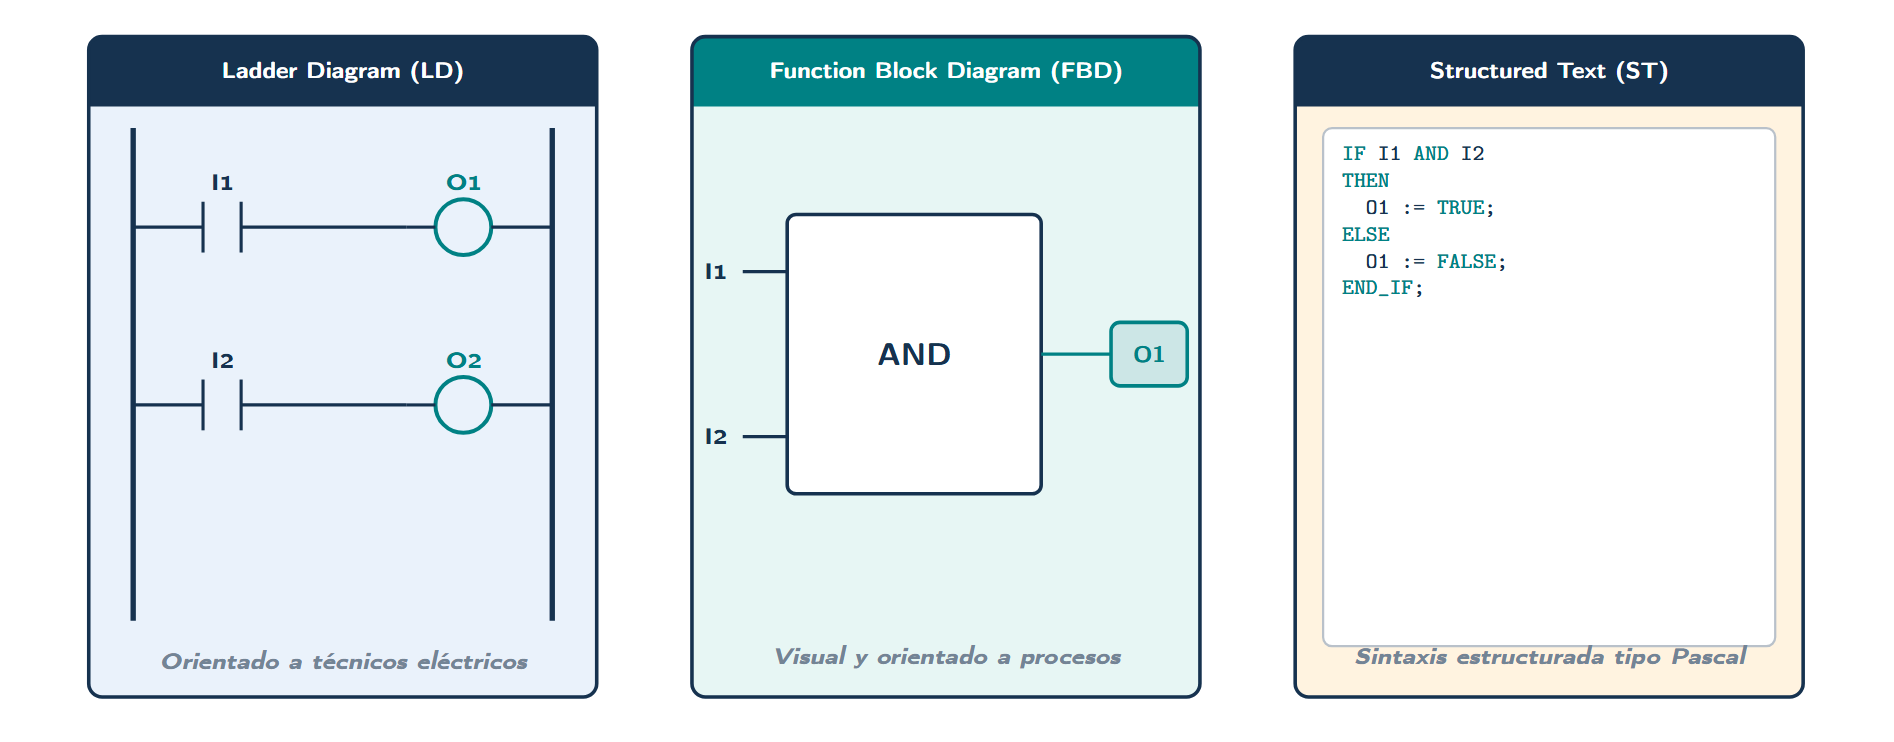
\includegraphics[width=\textwidth]{norma IEC 61131-3.png}
    \caption{Representación comparativa de los lenguajes LD, FBD y ST según IEC~61131-3. Fuente: Autora.}
    \label{fig:iec61131}
\end{figure}

\section{Arduino Opta como base tecnológica}
\label{sec:opta}

El Arduino Opta WiFi es un micro-PLC de grado industrial desarrollado por Arduino en colaboración con Finder~\cite{ref1}. Combina la accesibilidad y el amplio ecosistema de herramientas del entorno Arduino con características propias de equipos de automatización industrial, lo que lo posiciona como una plataforma idónea para entornos educativos orientados a la enseñanza de automatización.

\begin{figure}[H]
    \centering
    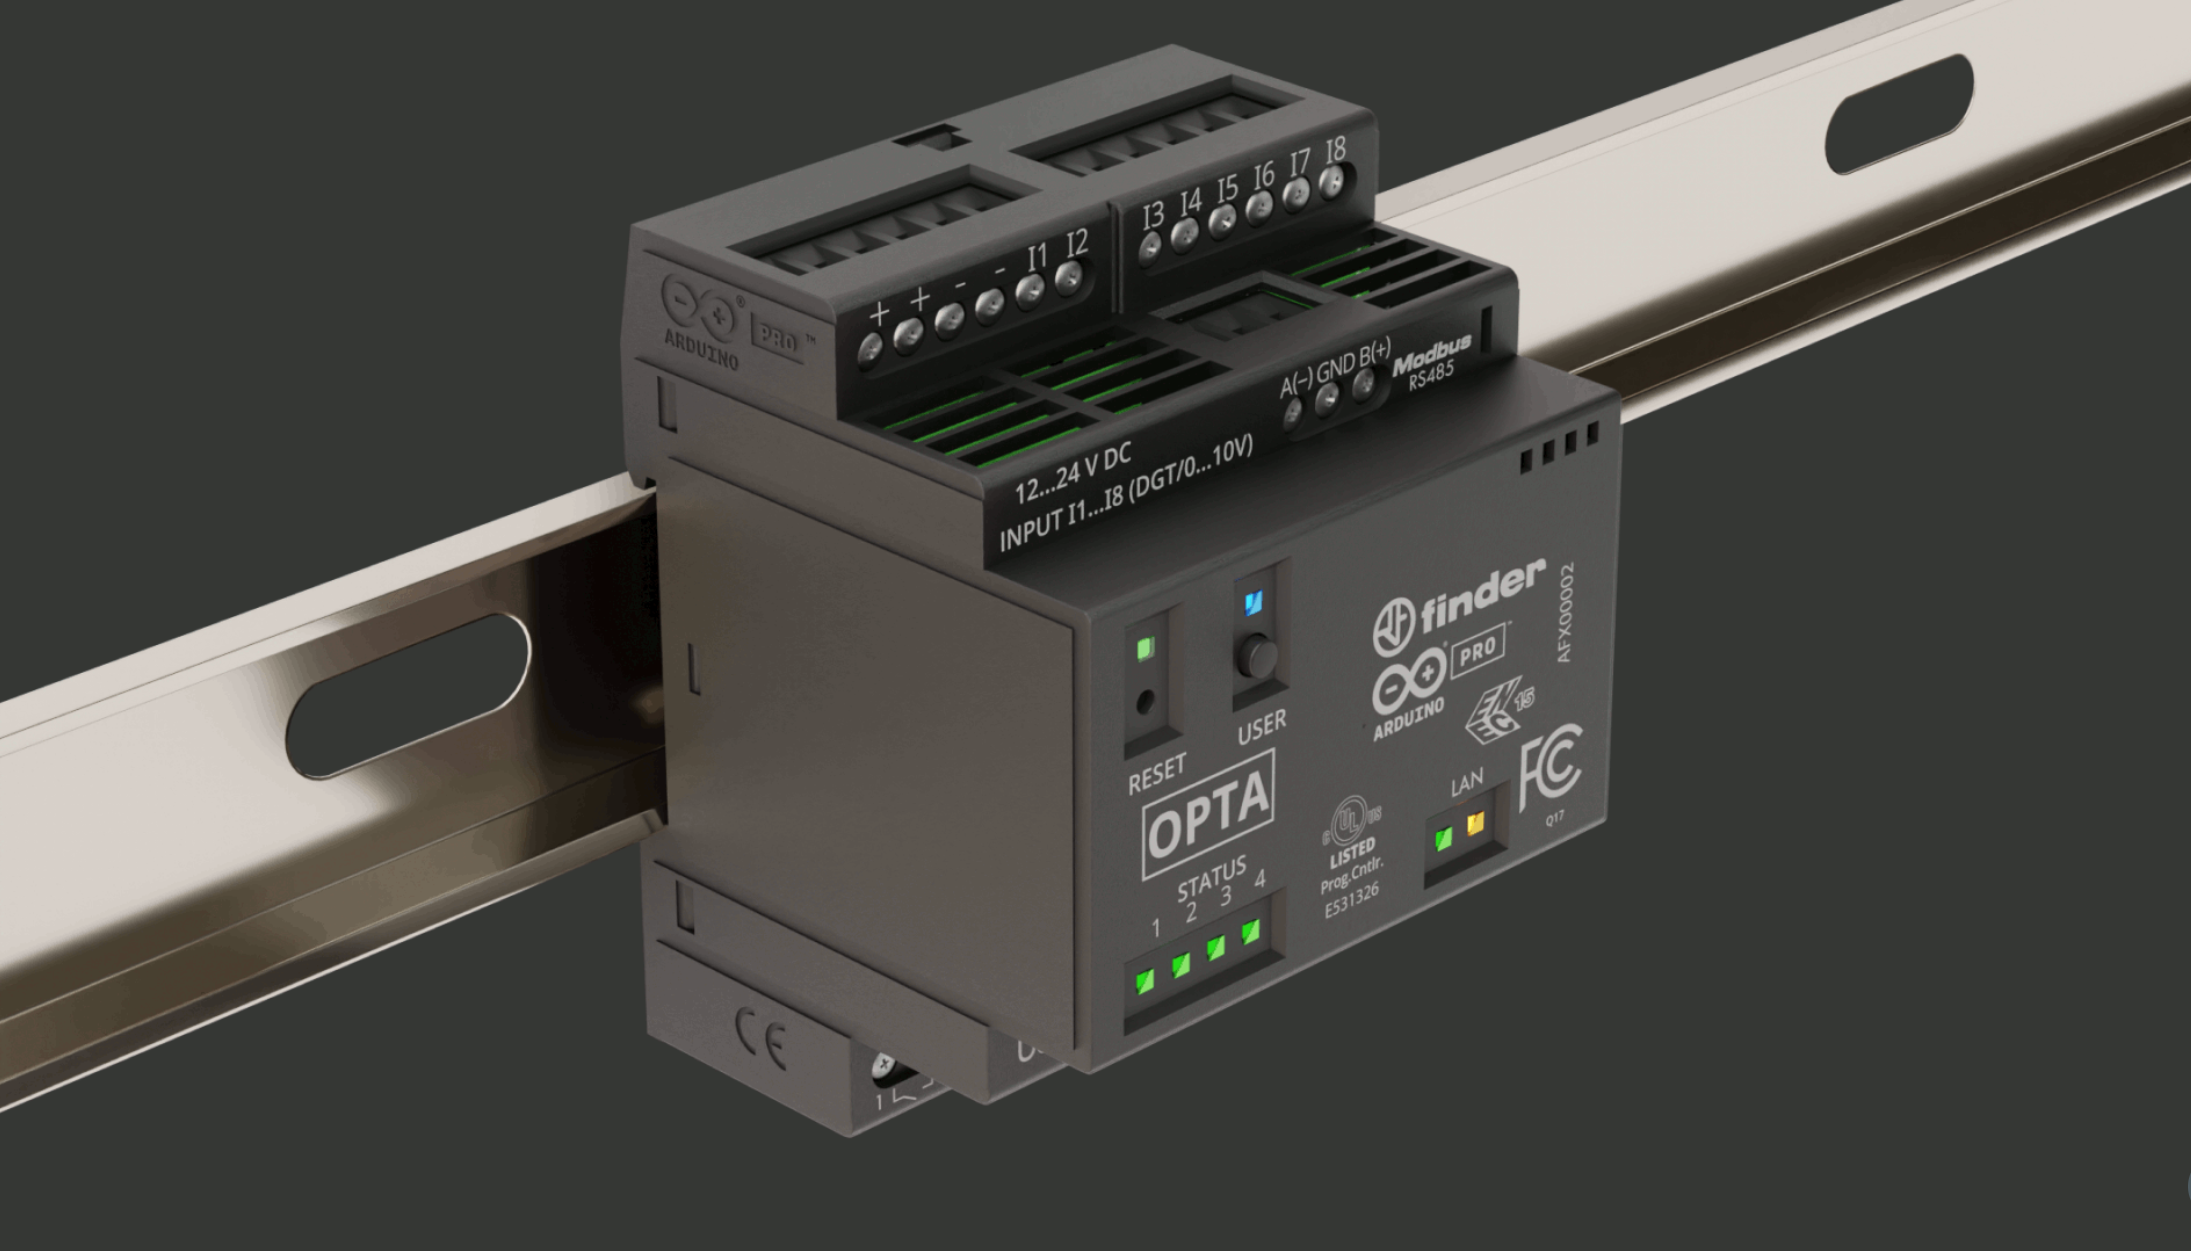
\includegraphics[width=0.9\textwidth]{Arduino_OPTA_Estetico.png}
    \caption{Arduino Opta WiFi~\cite{ref8}.}
    \label{fig:opta_estetico}
\end{figure}

\subsection{Especificaciones principales}

Las características técnicas del Arduino Opta WiFi más relevantes para el proyecto son las siguientes~\cite{ref1, ref8}:

\begin{itemize}
    \item \textbf{Entradas digitales:} 8 canales, rango 0--24 V DC, para contactos secos y sensores de tipo PNP; un sensor NPN requiere una resistencia de polarización externa.
    \item \textbf{Salidas de relé:} 4 canales de contacto seco (normalmente abierto), 250 VAC / 5 A por canal.
    \item \textbf{Conectividad:} WiFi 802.11 b/g/n, Bluetooth Low Energy y Ethernet 10/100 Mbps.
    \item \textbf{Interfaz RS-485:} puerto serie semidúplex con bornes A($-$), B($+$) y GND, compatible con el protocolo Modbus RTU (sección~\ref{subsec:modbus}).
    \item \textbf{Puerto USB-C:} para programación y comunicación con el PC.
    \item \textbf{Puerto AUX:} conexión lateral para encadenar hasta cinco módulos de expansión mediante bus de comunicación dedicado.
    \item \textbf{Programación:} compatible con Arduino IDE (C/C++) y PLC IDE de Arduino (lenguajes LD, FBD y ST según IEC~61131-3).
\end{itemize}

\subsection{Módulos del sistema}

El núcleo del sistema es el Arduino PLC Starter Kit (AKX00051)~\cite{ref2}, que incluye el Arduino Opta WiFi junto con los módulos DIN Simul8 y DIN Celsius, que se conectan al Opta mediante borneras de tornillo. Adicionalmente, el proyecto incorpora el módulo de expansión analógica AFX00007, adquirido por separado y conectado al Opta por el bus AUX, que amplía las capacidades de adquisición y generación de señales analógicas. La tabla~\ref{tab:modulos} resume los módulos del sistema y su función.

\begin{figure}[H]
    \centering
    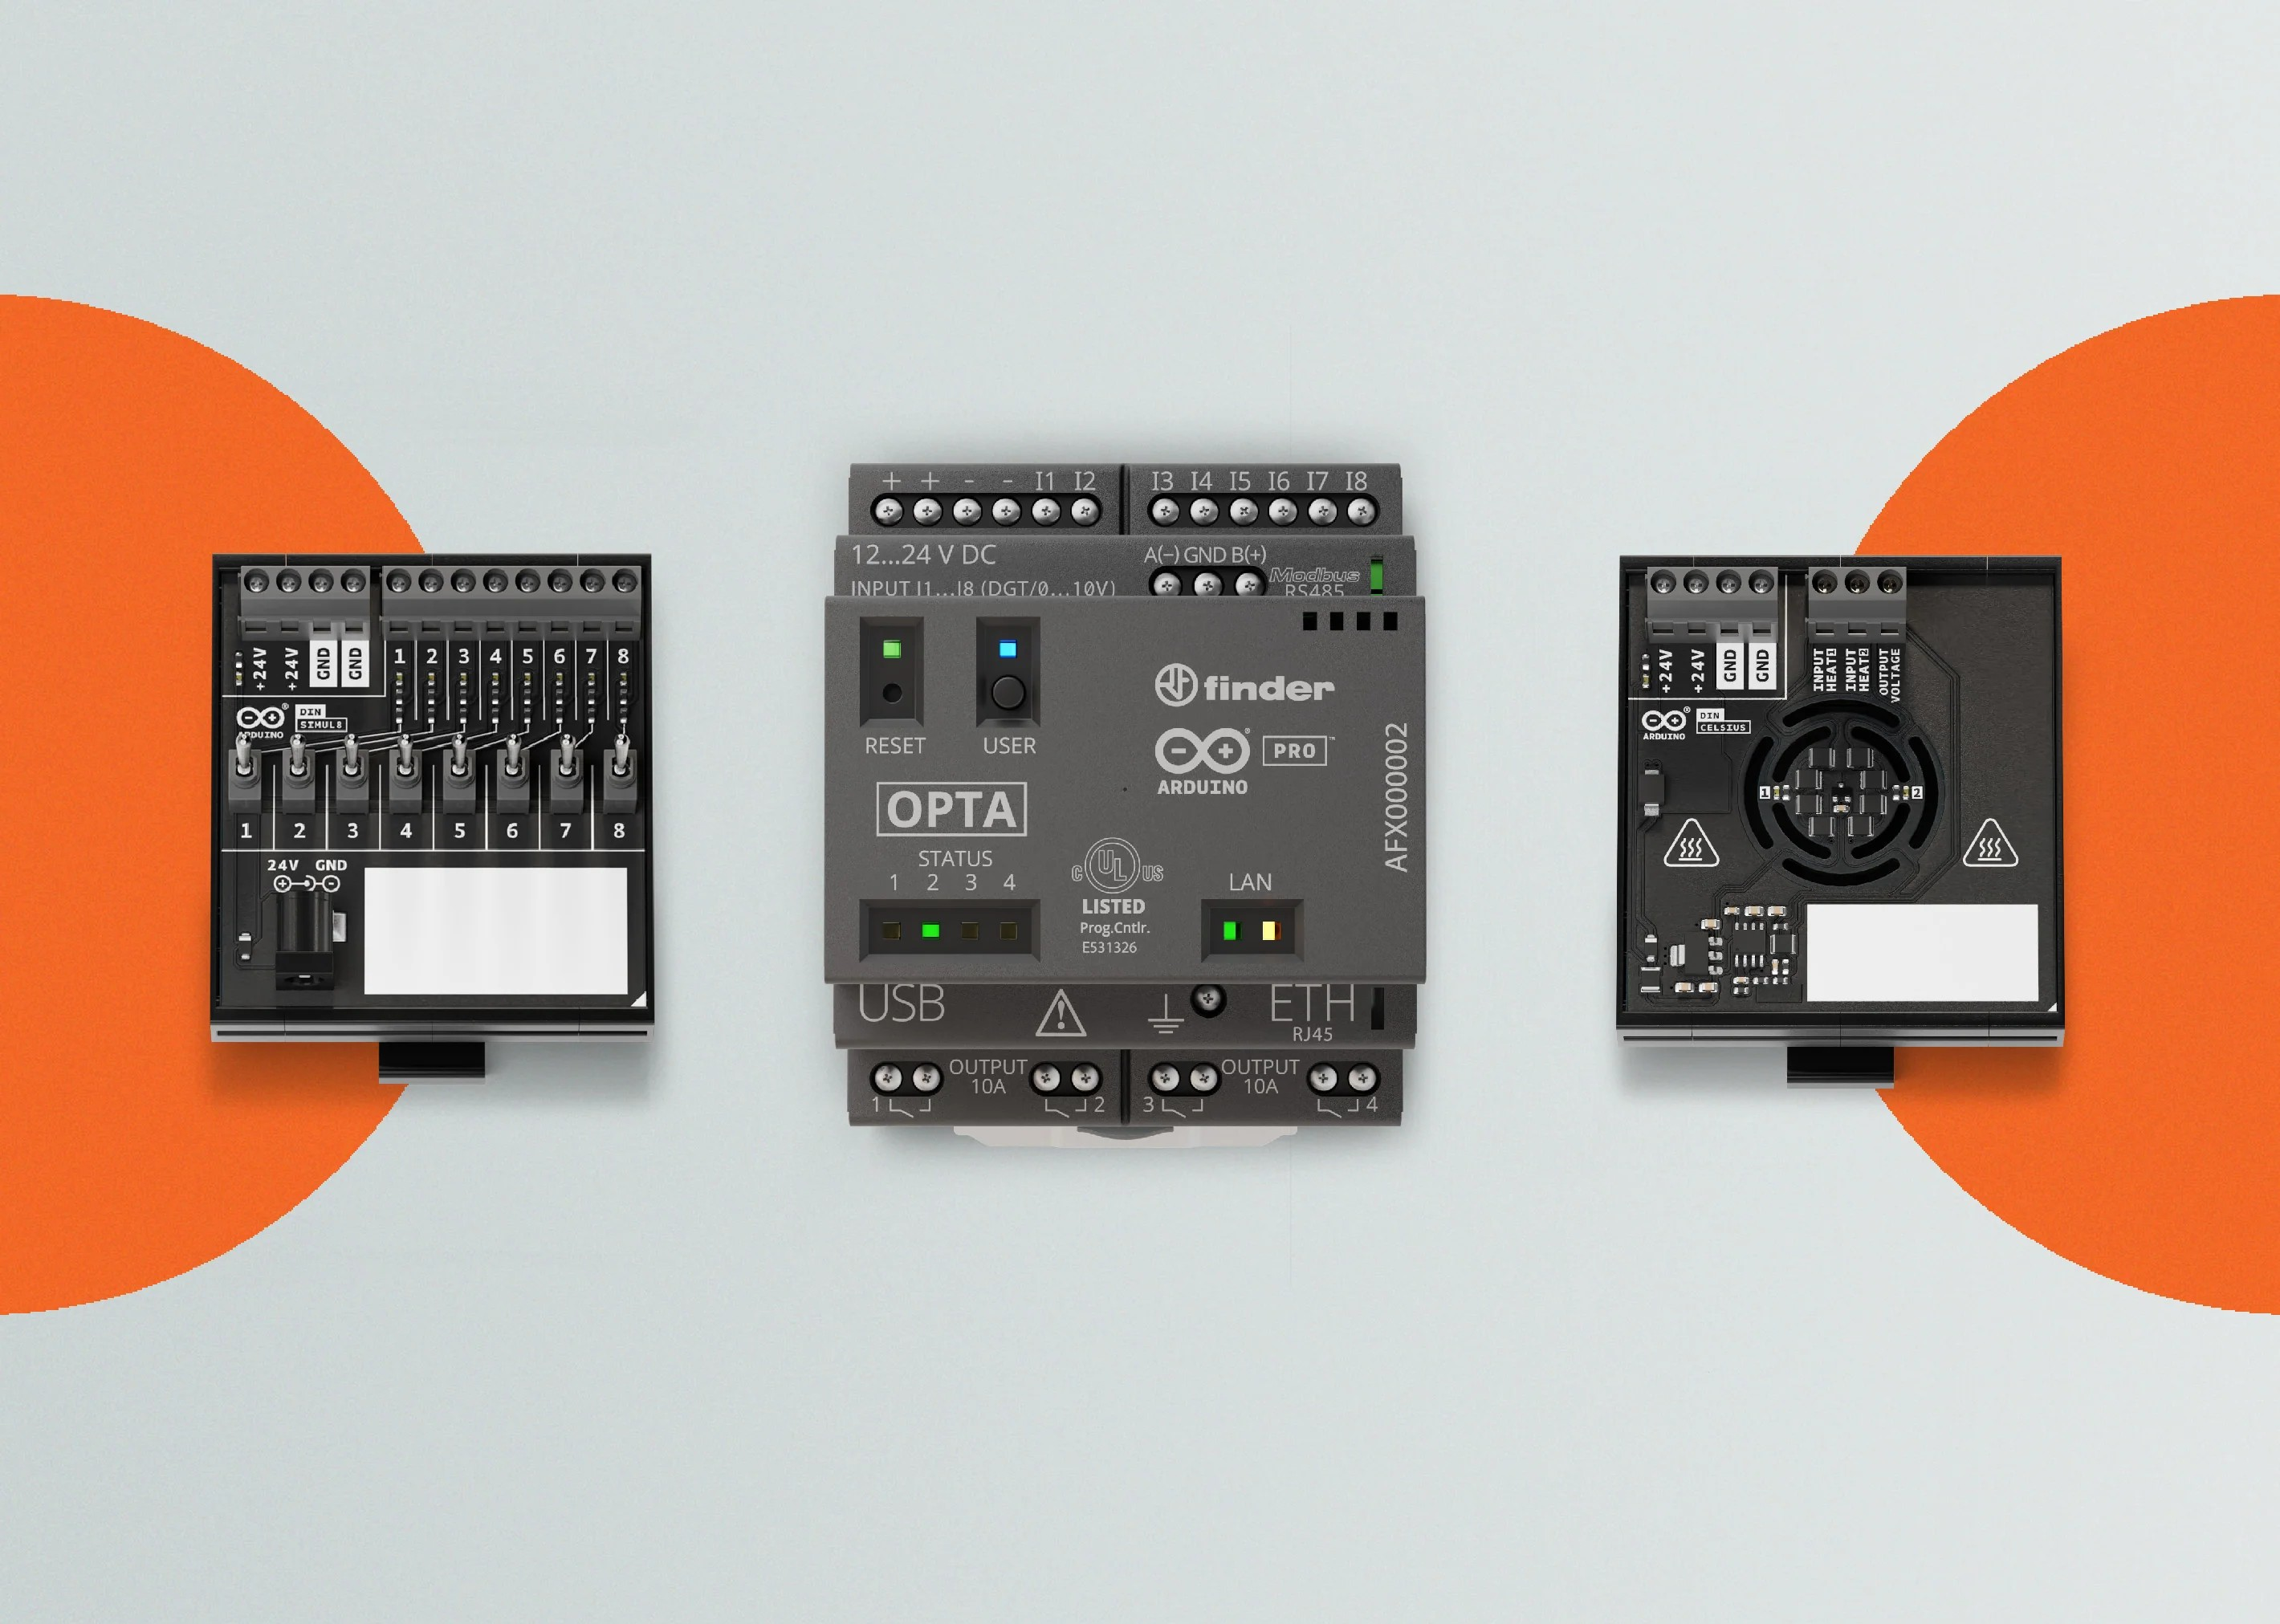
\includegraphics[width=0.85\textwidth]{PLC_Starter_Kit_Arduino_Store.jpg}
    \caption{Arduino PLC Starter Kit (AKX00051): Arduino Opta WiFi, módulo DIN Simul8 y módulo DIN Celsius~\cite{ref2}.}
    \label{fig:plc_starter_kit}
\end{figure}

\begin{table}[H]
\centering
\caption{Módulos del sistema de la plataforma didáctica.}
\label{tab:modulos}
\renewcommand{\arraystretch}{1.3}
\begin{tabularx}{\textwidth}{|>{\bfseries}p{3cm}|X|p{3.5cm}|}
\hline
\filacolor{TableGray}
\textbf{Módulo} & \textbf{Función} & \textbf{Terminales} \\
\hline
\filacolor{TableGray}
\multicolumn{3}{|l|}{\textit{Incluidos en el Arduino PLC Starter Kit (AKX00051)}} \\
\hline
SIMUL8 & 8 interruptores manuales que, al encenderse, entregan la tensión de alimentación del módulo (24~V DC) hacia las entradas I1--I8 del Opta. Recibe además la alimentación de 24~V por su conector de barril y la distribuye por borneras. Herramienta didáctica que permite probar lógica de control sin necesidad de sensores físicos. & 8 salidas de interruptor, +24~V y GND \\
\hline
CELSIUS & Pequeño laboratorio de temperatura: dos circuitos calefactores independientes de 24~V (unos 120~mW cada uno) y un sensor TMP236 en el centro de la placa, con salida analógica de 0--10~V. Rango del sensor: $-$10 °C a $+$125 °C ($\pm$2,5 °C). No se monta sobre el panel de control; se emplea como sensor de prueba externo en las prácticas de temperatura, conectado al conjunto únicamente cuando la práctica lo requiere~\cite{ref37}. & 2 entradas de calefactor (24~V), salida del sensor, GND \\
\hline
\filacolor{TableGray}
\multicolumn{3}{|l|}{\textit{Módulo de expansión adicional (adquirido por separado)}} \\
\hline
AFX00007 & Módulo analógico: 6 entradas programables (0--10 V / 4--20 mA / PT100), 2 salidas analógicas (0--10 V o 4--20 mA) y 4 salidas PWM. & I1--I6, O1--O2, P1--P4 \\
\hline
\end{tabularx}
\end{table}

\begin{figure}[H]
    \centering
    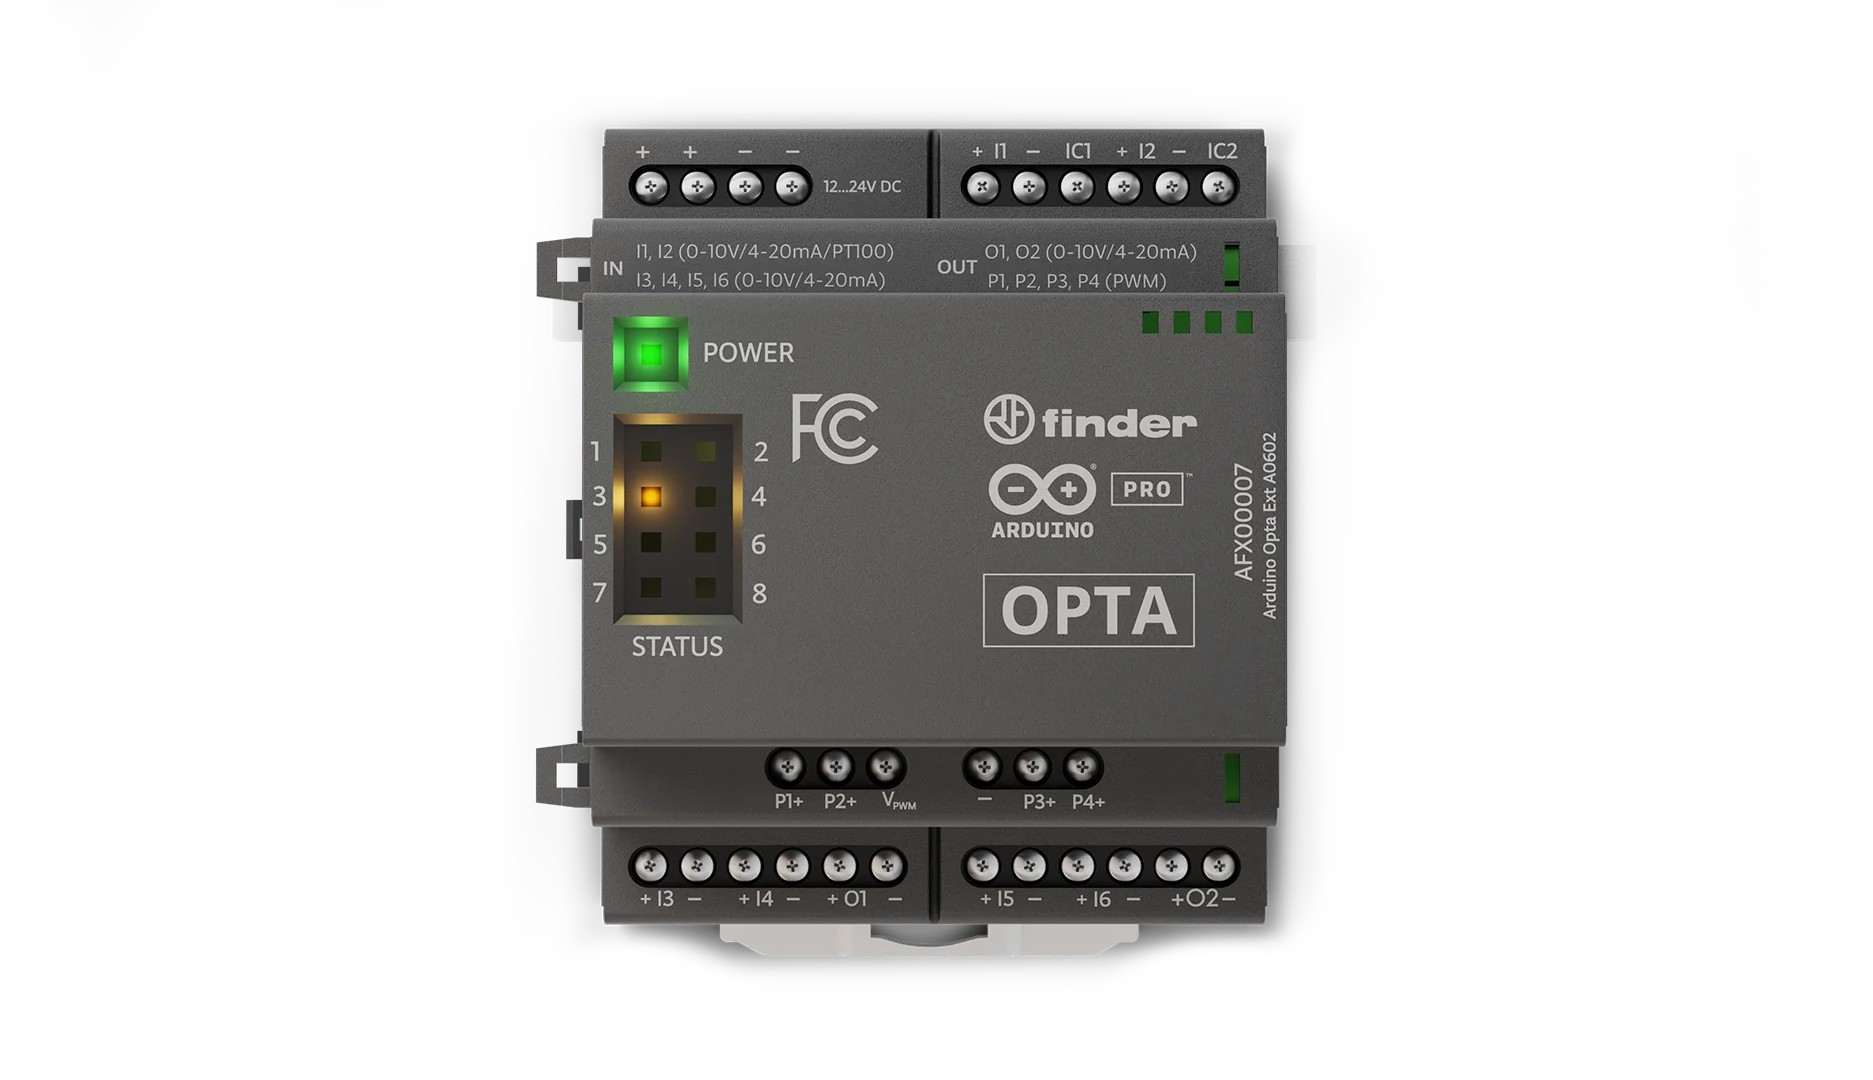
\includegraphics[width=0.75\textwidth]{AFX00007_Expansion_Modules.jpg}
    \caption{Módulo de expansión analógica AFX00007 (adquirido por separado)~\cite{ref35}.}
    \label{fig:afx00007}
\end{figure}

\subsection{Interfaz de conexiones}

\begin{figure}[H]
    \centering
    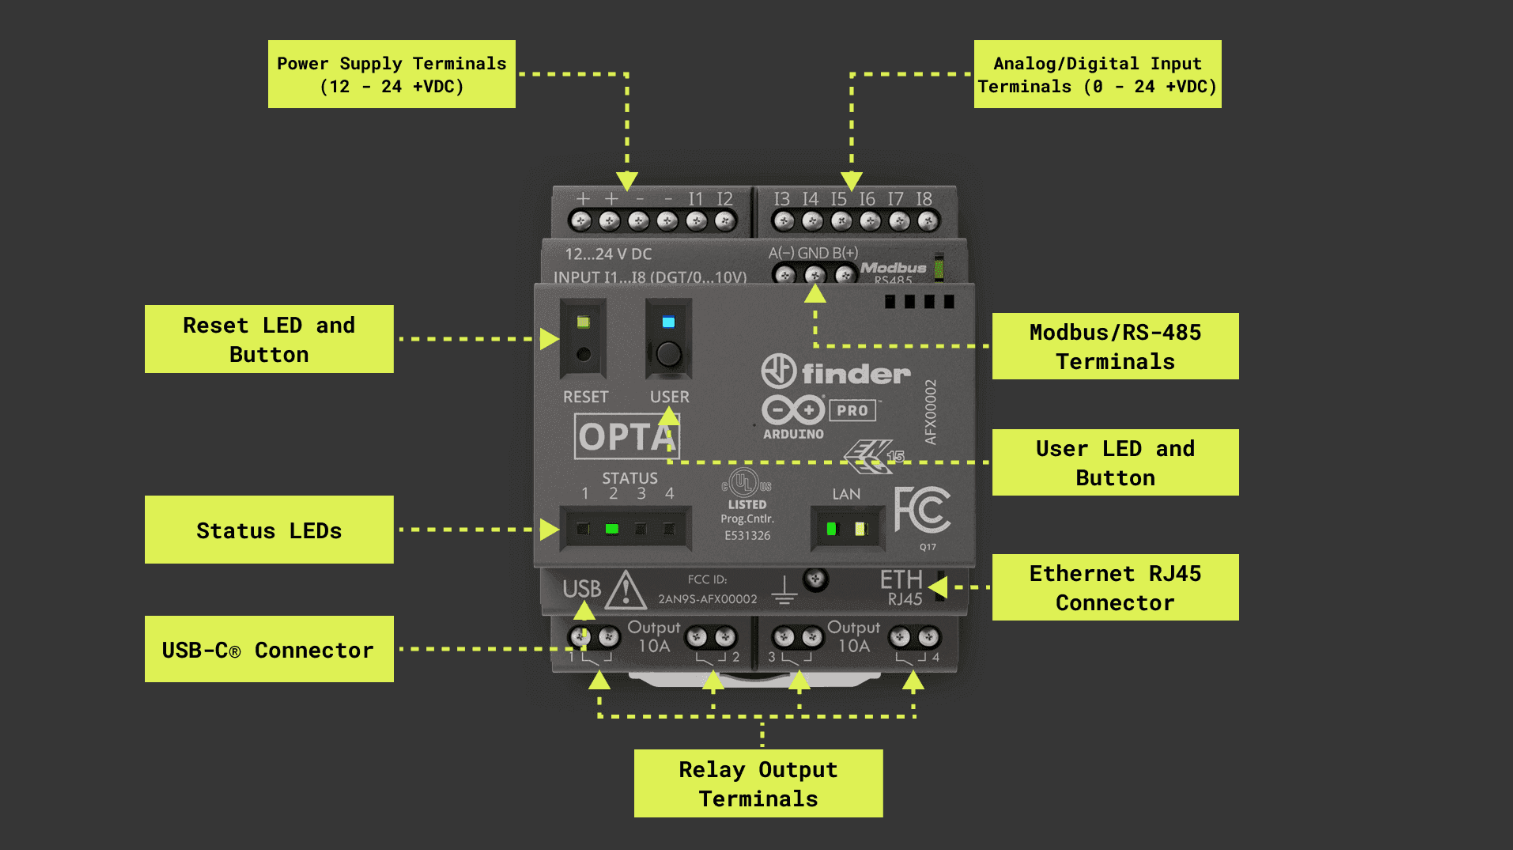
\includegraphics[width=0.9\textwidth]{Arduino_OPTA_Detallado.png}
    \caption{Diagrama de conexiones del Arduino Opta WiFi~\cite{ref8}.}
    \label{fig:opta_detallado}
\end{figure}

La figura~\ref{fig:opta_detallado} muestra la disposición física de los terminales del Arduino Opta. Las entradas digitales aceptan señales de 0 a 24 V DC; las salidas son contactos secos de relé que requieren alimentación externa en serie con la carga; y el puerto AUX lateral permite la conexión en cadena de módulos de expansión como el AFX00007 de la tabla~\ref{tab:modulos}. Junto a las entradas se ubican además los bornes A($-$), GND y B($+$) de la interfaz RS-485, que se describe en la sección siguiente.

\subsection{Comunicación industrial: RS-485 y Modbus}
\label{subsec:modbus}

Además de las entradas y salidas descritas, el Arduino Opta WiFi incorpora una interfaz de comunicación serie RS-485 y es compatible con el protocolo Modbus, tanto en su versión RTU sobre RS-485 como en su versión TCP sobre Ethernet~\cite{ref8}. Aunque esta capacidad no se implementa físicamente en el presente proyecto (sección~\ref{sec:limitaciones}), se documenta aquí por la importancia que tiene la comunicación entre dispositivos en la automatización industrial y porque constituye la vía natural de crecimiento de la plataforma.

\subsubsection{Interfaz física RS-485}

RS-485 es un estándar eléctrico de transmisión serie que utiliza un par de líneas diferenciales. Al transmitir la información como la diferencia de tensión entre ambas líneas, y no respecto a tierra, el ruido que se induce por igual en los dos conductores se cancela en el receptor. Esto le da una buena inmunidad al ruido y permite enlaces más largos que otras interfaces serie, lo que la hace adecuada para el piso de una planta industrial~\cite{ref29}. Se trata además de un bus multipunto, en el que varios transmisores y receptores pueden compartir la misma línea, y la alta impedancia de entrada de los receptores permite conectar más dispositivos sobre el mismo par~\cite{ref8}.

Es importante notar que RS-485 define únicamente las características eléctricas de la línea, no la forma de interpretar los datos. Para que dos equipos se entiendan se requiere un protocolo de comunicación por encima de ella, y Modbus RTU es uno de los más empleados con este fin~\cite{ref29}.

En el Arduino Opta, la interfaz opera en modo semidúplex (\textit{half-duplex}), es decir, puede enviar o recibir, pero no ambas cosas a la vez. Sus líneas se identifican como A($-$) y B($+$), junto con un borne GND de referencia. Arduino advierte que el etiquetado de estas líneas varía entre fabricantes, por lo que, si la comunicación no se establece con otro equipo, la primera prueba es intercambiar A y B; invertir la polaridad no daña el dispositivo~\cite{ref8}. El Opta no incluye resistencias de terminación internas, de modo que deben añadirse en los extremos del bus cuando la especificación de Modbus lo requiera. Para el cableado, el fabricante recomienda par trenzado (STP o UTP) con impedancia característica de 100 a 130~$\Omega$~\cite{ref30}. La figura~\ref{fig:rs485_opta} muestra la conexión entre dos equipos; los tres bornes se unen uno a uno, y cada Opta conserva su propia alimentación.

\begin{figure}[H]
    \centering
    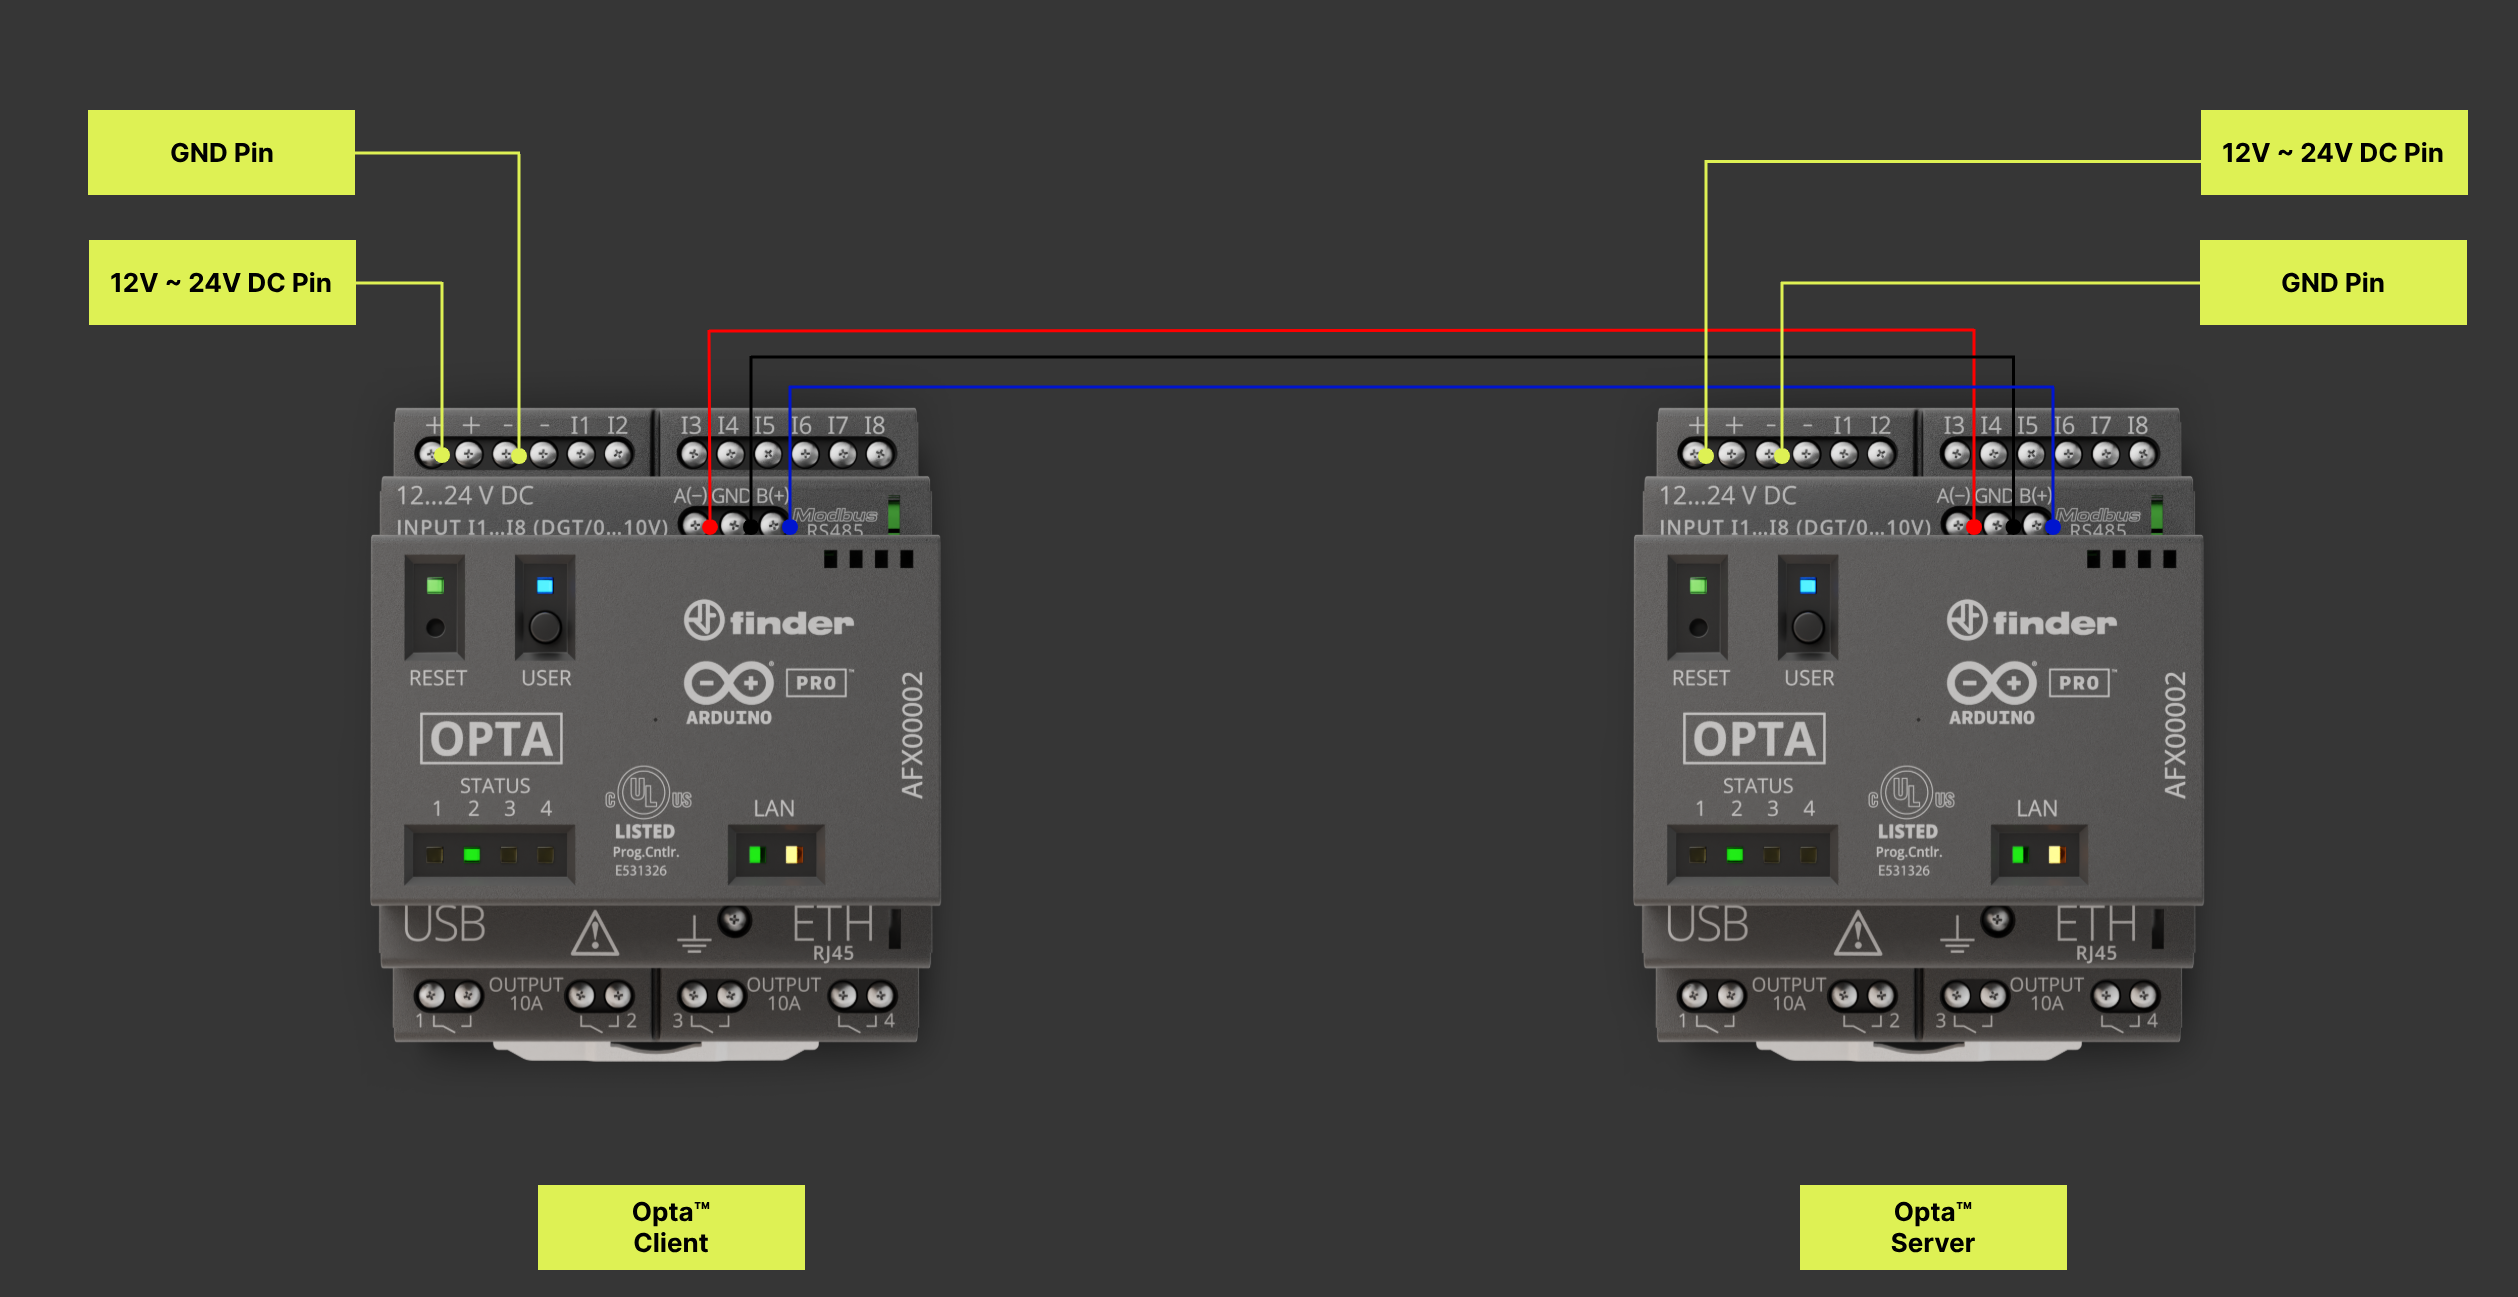
\includegraphics[width=0.95\textwidth]{RS-485.png}
    \caption{Conexión de dos Arduino Opta mediante la interfaz RS-485: bornes A($-$), GND y B($+$) unidos entre el equipo cliente y el equipo servidor, cada uno con su alimentación de 12--24~V~DC~\cite{ref30}.}
    \label{fig:rs485_opta}
\end{figure}

\subsubsection{Protocolo Modbus}

Modbus es un protocolo de comunicación abierto y libre de regalías, publicado por Modicon (hoy Schneider Electric) en 1979. Con el tiempo se convirtió en un estándar \textit{de facto} para la comunicación entre PLC y otros equipos industriales, y es común en sistemas de automatización industrial, en la gestión de edificios y en la conexión de unidades remotas con sistemas SCADA~\cite{ref30}.

Su funcionamiento sigue una arquitectura cliente/servidor (en la terminología antigua, maestro/esclavo). El cliente es el único equipo que inicia la comunicación. Envía una petición dirigida a un servidor identificado por su dirección, y el servidor responde con la información solicitada o confirma la escritura. En una misma red puede haber varios servidores, pero un solo cliente~\cite{ref30}. En una línea serie, las direcciones válidas de servidor van de 1 a 247, y la dirección 0 se reserva para mensajes de difusión que todos los servidores reciben sin responder~\cite{ref31}.

Los datos que un servidor pone a disposición se organizan en cuatro tipos, resumidos en la tabla~\ref{tab:modbus_datos}~\cite{ref32}. Un servidor puede ser otro PLC, pero también un variador de frecuencia, un medidor de energía o un sensor con interfaz Modbus.

\begin{table}[H]
\centering
\caption{Tipos de datos del modelo Modbus. Fuente: Autora.}
\label{tab:modbus_datos}
\renewcommand{\arraystretch}{1.3}
\begin{tabularx}{\textwidth}{|>{\bfseries\raggedright\arraybackslash}p{4.6cm}|p{1.5cm}|>{\raggedright\arraybackslash}p{2.2cm}|>{\raggedright\arraybackslash}X|}
\hline
\filacolor{TableGray}
\textbf{Tipo} & \textbf{Tamaño} & \textbf{Acceso} & \textbf{Uso típico} \\
\hline
Bobinas (\textit{coils}) & 1 bit & Lectura y escritura & Salidas digitales, órdenes de marcha o paro \\
\hline
Entradas discretas (\textit{discrete inputs}) & 1 bit & Solo lectura & Estado de entradas digitales \\
\hline
Registros de entrada (\textit{input registers}) & 16 bits & Solo lectura & Mediciones analógicas \\
\hline
Registros de retención (\textit{holding registers}) & 16 bits & Lectura y escritura & Consignas y parámetros de configuración \\
\hline
\end{tabularx}
\end{table}

En la versión RTU, cada mensaje se transmite como una trama binaria compuesta por la dirección del servidor (1 byte), el código de función que indica la operación (1 byte), los datos y una verificación de redundancia cíclica (CRC) de 16 bits que permite al receptor detectar errores de transmisión. El inicio y el fin de cada trama se reconocen por un silencio en la línea de al menos 3,5 tiempos de carácter~\cite{ref31}. Por esta razón, al configurar la interfaz RS-485 del Opta se fijan retardos antes y después de cada transmisión calculados a partir de la velocidad de comunicación. Las velocidades típicas son 9600 y 19\,200~bit/s; el ejemplo del fabricante usa 19\,200~bit/s con formato de 8 bits de datos, paridad par y 1 bit de parada~\cite{ref30}.

La versión TCP transporta los mismos mensajes sobre una red Ethernet. Opera en dúplex completo y se integra con la infraestructura de red existente, lo que facilita la comunicación a mayor distancia~\cite{ref8}.

\subsubsection{Herramientas de programación}

Arduino ofrece dos caminos para trabajar con Modbus en el Opta. En el Arduino IDE, las bibliotecas ArduinoRS485 y ArduinoModbus resuelven la configuración de la interfaz y el intercambio de bobinas y registros mediante código C/C++~\cite{ref29, ref30}. En el PLC IDE, el rol del equipo (cliente o servidor), la velocidad, el formato serie y los nodos de la red se definen en la configuración del proyecto; el programa, escrito en cualquiera de los lenguajes IEC~61131-3, solo lee y escribe variables predefinidas, y el entorno se encarga de la transferencia de datos~\cite{ref33}. Este segundo camino es el más coherente con el enfoque didáctico de la plataforma, porque el estudiante no necesita programar el protocolo para usarlo.

\subsubsection{Proyección en la plataforma}

La interfaz RS-485 abre varias líneas de crecimiento para la plataforma. Permitiría conectar varias plataformas entre sí, con un Opta como cliente que coordina a los demás como servidores; integrar equipos de campo con interfaz Modbus, como variadores de frecuencia, medidores de energía o sensores industriales; y enlazar la plataforma con un sistema de supervisión tipo SCADA. Con ello, el estudiante podría pasar del control de un proceso aislado a la comunicación entre equipos, una competencia central en la automatización industrial actual. Los bornes RS-485 ya están presentes en el controlador seleccionado, por lo que estas ampliaciones no requieren cambiar la unidad de control.

\subsection{Accesibilidad económica y transferibilidad de competencias}

Un aspecto determinante del Arduino Opta como base tecnológica para una plataforma didáctica es su relación costo-beneficio frente a los sistemas PLC industriales convencionales. Los equipos de fabricantes como Siemens, Allen-Bradley o Schneider Electric (aunque robustos y ampliamente implantados en la industria) tienen un precio de adquisición que puede superar en un orden de magnitud al del Arduino PLC Starter Kit~\cite{ref2}, lo que constituye una barrera económica significativa para los laboratorios con presupuesto limitado.

El Arduino Opta se sitúa en un segmento de costo sensiblemente inferior sin sacrificar la compatibilidad con los estándares industriales más relevantes. En particular, su soporte para los lenguajes IEC~61131-3 mediante el PLC IDE de Arduino garantiza que las competencias adquiridas en el entorno educativo (Ladder Diagram, Function Block Diagram y Structured Text) sean directamente transferibles al trabajo con PLC industriales de cualquier fabricante que respete el mismo estándar~\cite{ref4}. Esta transferibilidad es un atributo de alto valor pedagógico, porque el estudiante aprende con una herramienta accesible y lleva esas habilidades al entorno productivo sin necesidad de una reinducción técnica profunda.

% -------------------------------------------------
\section{Estado del arte}
\label{sec:estado}
% -------------------------------------------------

La enseñanza de la automatización industrial mediante plataformas didácticas ha evolucionado considerablemente en las últimas décadas. La literatura identifica cuatro enfoques principales, cada uno con características, ventajas y limitaciones particulares que condicionan su aplicación en entornos educativos~\cite{ref3,ref4,ref5,ref6}. En las subsecciones siguientes se describen y analizan dichos enfoques, y se establece el posicionamiento del presente proyecto en relación con el estado del arte.

\subsection{Kits educativos comerciales}

Los kits educativos comerciales integran en un único sistema un controlador PLC, módulos de experimentación y guías de práctica estructuradas. Ejemplos representativos incluyen el Arduino PLC Starter Kit~\cite{ref2} y sistemas equivalentes de fabricantes como Siemens, Festo y Allen-Bradley.

Estos kits facilitan la implementación rápida de prácticas en el laboratorio y suelen incluir documentación pedagógica desarrollada para el docente. Sin embargo, presentan limitaciones en cuanto a la flexibilidad de adaptación, ya que el estudiante trabaja con escenarios predefinidos por el fabricante y tiene escasa posibilidad de modificar la arquitectura del sistema o conectar elementos de campo propios sin intervenir el hardware principal~\cite{ref3}. Investigaciones recientes documentan el uso de PLCs industriales comerciales de gama media (como el Siemens S7-1200) en entornos de educación técnica, lo que evidencia su pertinencia formativa pero también el reto económico que representan para instituciones con presupuesto limitado~\cite{ref12}.

\subsection{Laboratorios modulares físicos}

Los laboratorios modulares físicos separan la unidad de control central de módulos de proceso o campo intercambiables. Esta arquitectura permite utilizar una misma infraestructura de control para múltiples prácticas distintas, simplemente sustituyendo o reconfigurando el módulo de campo conectado.

Vázquez-González et al.~\cite{ref4} proponen una infraestructura común para laboratorios de programación PLC en modalidades física, virtual y remota. Su trabajo demuestra que la separación entre la unidad de control y el módulo de campo favorece la reutilización de los recursos del laboratorio, la escalabilidad de las prácticas y la reducción de costos de mantenimiento. Este enfoque es el más directamente relacionado con la arquitectura del presente proyecto. En esa misma dirección, Al-Yaman et al.~\cite{ref10} presentan una solución modular de bajo costo que opera a aproximadamente el 27\,\% del costo de un sistema convencional, con capacidad para atender múltiples pares de estudiantes simultáneamente mediante kits de aplicación intercambiables, lo que valida la viabilidad económica del enfoque modular físico en contextos académicos con recursos limitados.

\subsection{Laboratorios virtuales y remotos}

Los laboratorios virtuales y remotos permiten programar, simular y validar lógica de control sin acceso físico al hardware. Bellmunt et al.~\cite{ref5} describen un curso de programación PLC a distancia basado en una celda de manufactura flexible accesible remotamente mediante interfaz web, demostrando que es posible desarrollar competencias de programación sin presencia física en el laboratorio. En una línea similar, Vargas et al.~\cite{ref11} integran el entorno de simulación Factory~I/O en un currículo por competencias para la enseñanza de automatización industrial con PLC, evaluando su eficacia en un curso de posgrado y confirmando el potencial de la simulación como complemento a la formación presencial.

Si bien estos entornos amplían significativamente el acceso a la formación en automatización (especialmente en contextos de educación a distancia o con recursos limitados), presentan una limitación relevante para la formación técnica integral, pues el estudiante no experimenta el proceso físico de cableado, conexión de señales e instrumentación, que constituye una competencia esencial en el desempeño profesional del ingeniero~\cite{ref4,ref5,ref11}.

\subsection{Gemelos digitales aplicados a educación}

Los gemelos digitales (\textit{digital twins}) vinculan una planta física real con una réplica virtual sincronizada, permitiendo supervisión, análisis y experimentación sobre el modelo digital con impacto directo en el sistema físico real. Liljaniemi y Paavilainen~\cite{ref6} documentan la aplicación de esta tecnología en entornos educativos de ingeniería, destacando su alineación con los principios de la Industria 4.0 y las posibilidades que ofrece para el análisis de datos y la optimización de procesos.

Esta aproximación representa el estado del arte más avanzado en plataformas didácticas de automatización. No obstante, su implementación requiere una mayor complejidad técnica y de infraestructura computacional, lo que puede limitar su adopción en laboratorios educativos con recursos moderados~\cite{ref6}.

\subsection{Análisis comparativo}

La tabla~\ref{tab:estadoarte} sintetiza los cuatro enfoques identificados en la literatura, con sus principales aportes y limitaciones.

\begin{table}[H]
\centering
\caption{Comparativa de enfoques en plataformas didácticas de automatización industrial.}
\label{tab:estadoarte}
\renewcommand{\arraystretch}{1.35}
\begin{tabularx}{\textwidth}{|>{\bfseries}p{3.5cm}|X|p{5.5cm}|}
\hline
\filacolor{TableGray}
\textbf{Enfoque} & \textbf{Descripción} & \textbf{Aporte / Limitación} \\
\hline
Kits educativos comerciales & Integran PLC, módulos de experimentación y guías de práctica estructuradas~\cite{ref2,ref3}. & Facilitan implementación; menor flexibilidad de adaptación. \\
\hline
Laboratorios modulares físicos & Separan la unidad de control de módulos de campo intercambiables~\cite{ref4}. & Favorecen reutilización, escalabilidad y mantenimiento. \\
\hline
Laboratorios virtuales y remotos & Permiten programar y validar lógica de control a distancia~\cite{ref4,ref5}. & Amplían el acceso; limitan la experiencia física de cableado e instrumentación. \\
\hline
Gemelos digitales & Vinculan una planta física con una réplica virtual para supervisión y análisis~\cite{ref6}. & Alineados con Industria 4.0; requieren mayor complejidad técnica e infraestructura. \\
\hline
\end{tabularx}
\end{table}

\subsection{Síntesis y posicionamiento del proyecto}

El análisis del estado del arte revela un interés creciente en la literatura por plataformas didácticas que combinen hardware industrial real, modularidad y conectividad~\cite{ref3,ref4}. Los laboratorios modulares físicos emergen como el enfoque más adecuado para el contexto de este proyecto, al priorizar la reutilización del sistema base y la flexibilidad para diferentes prácticas experimentales sin necesidad de intervenir el hardware principal.

La propuesta de este trabajo (un panel de control con Arduino Opta como plataforma principal) se alinea con este enfoque y lo extiende incorporando un micro-PLC de grado industrial accesible. El diseño busca que el estudiante desarrolle competencias de programación PLC según IEC~61131-3, conexión de señales industriales e instrumentación a 24 V DC, en un entorno que garantice seguridad eléctrica, reutilización y adaptabilidad a múltiples escenarios de práctica.

Adicionalmente, el uso del Arduino Opta como plataforma base incorpora una dimensión económica que distingue esta propuesta de los enfoques basados en PLC industriales convencionales, ya que su costo significativamente menor la hace viable para instituciones con recursos limitados, mientras que su compatibilidad con IEC~61131-3 asegura que las competencias adquiridas sean transferibles al entorno industrial. El estudiante aprende a programar, configurar y operar un PLC real (con señales industriales estándar y lenguajes normativos) a una fracción del costo de una plataforma industrial equivalente~\cite{ref2,ref3}.

\section{FluidSIM y el módulo de interfaz EasyPort}
\label{sec:fluidsim_easyport}

El panel de control con Arduino Opta cubre la conexión de señales industriales reales a 24~V~DC, pero no puede alojar físicamente todos los actuadores (cilindros neumáticos, motores, electroválvulas, contactores) que un estudiante debe reconocer para completar su formación en automatización industrial. Para ampliar el alcance de las prácticas a escenarios eléctricos, neumáticos e hidráulicos sin esa limitación física, el proyecto incorpora una plataforma de simulación virtual basada en dos productos de Festo Didactic: el software FluidSIM y la interfaz de proceso EasyPort.

\subsection{FluidSIM}

FluidSIM es el software de Festo Didactic para la creación y simulación de diagramas de circuitos de neumática, hidráulica e ingeniería eléctrica. Cuenta con más de 25 años de desarrollo y más de 300\,000 instalaciones en todo el mundo, lo que lo convierte en una de las herramientas de referencia en la formación técnica en mecatrónica~\cite{ref28}. El software incluye bibliotecas de componentes neumáticos, hidráulicos y electrotécnicos que pueden combinarse entre sí, así como instrumentos de medición virtuales que permiten observar las variables de estado del circuito durante la simulación~\cite{ref28}.

Para este proyecto, FluidSIM permite que el estudiante diseñe y simule circuitos de control eléctricos, neumáticos o hidráulicos que representan actuadores industriales a 24~V~DC (sin necesidad de adquirir físicamente cada uno de esos actuadores) y valide su lógica de control sobre un modelo del proceso antes o en lugar de conectarlo a un elemento de campo real.

\subsection{Interfaz de proceso EasyPort}

El EasyPort USB (modelo D16A) es una interfaz de proceso de Festo Didactic diseñada para la transmisión bidireccional de señales de proceso en baja tensión (24~V~DC) entre un proceso real y un PC. Para evitar que el proceso influya sobre el PC, la transmisión de datos se realiza siempre mediante interfaces galvánicamente aisladas~\cite{ref27}.

\begin{figure}[H]
    \centering
    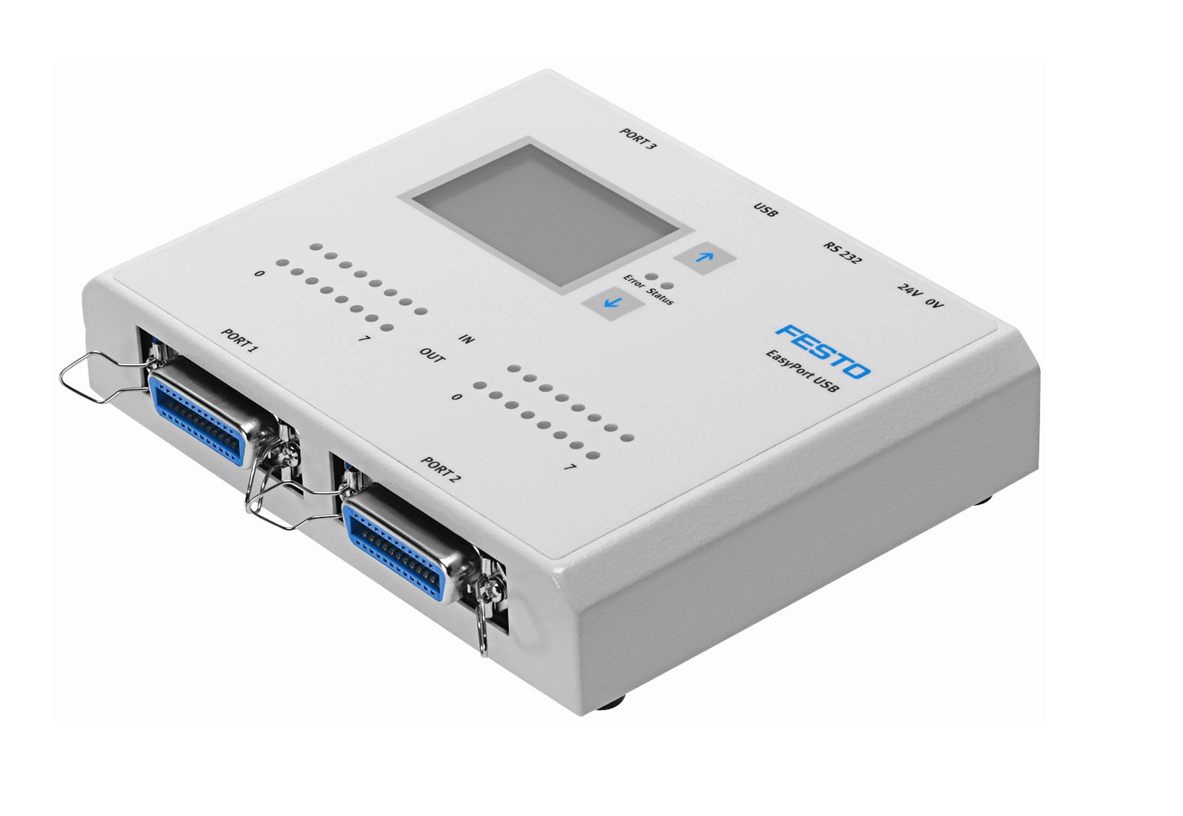
\includegraphics[width=0.6\textwidth]{EasyPort_perfil.png}
    \caption{Interfaz de proceso EasyPort USB de Festo Didactic~\cite{ref27}.}
    \label{fig:easyport}
\end{figure}

El manual del fabricante describe cuatro modos de aplicación para el EasyPort~\cite{ref27}:

\begin{itemize}
    \item Controlar un proceso real mediante un controlador que se ejecuta en el PC.
    \item Controlar un proceso simulado en el PC mediante un PLC real.
    \item Regular un proceso real desde el PC.
    \item Registrar y evaluar valores medidos de un proceso real.
\end{itemize}

El segundo modo (controlar un proceso simulado con un PLC real) es el que resulta pertinente para esta plataforma. En él, el Arduino Opta, programado por el estudiante con los lenguajes IEC~61131-3, gobierna un proceso representado en FluidSIM a través de las señales digitales y analógicas de 24~V~DC que intercambia con el EasyPort, en lugar de las señales de campo reales conectadas al panel de control, o además de ellas. El equipo expone tres puertos de conexión: los Puertos~1 y~2, cada uno con 8 entradas y 8 salidas digitales mediante conector SysLink de 24 pines según IEEE~488, y el Puerto~3, con las entradas y salidas analógicas~\cite{ref27}. La tabla~\ref{tab:easyport} resume las especificaciones técnicas relevantes para el proyecto.

\begin{table}[H]
\centering
\caption{Especificaciones técnicas de la interfaz de proceso EasyPort USB (modelo D16A)~\cite{ref27}.}
\label{tab:easyport}
\renewcommand{\arraystretch}{1.3}
\begin{tabularx}{\textwidth}{|>{\bfseries}p{4.5cm}|X|}
\hline
\filacolor{TableGray}
\textbf{Parámetro} & \textbf{Especificación} \\
\hline
Tensión de alimentación & 24~V~DC $\pm$10\,\% \\
\hline
Entradas digitales & 16 canales, 24~V~DC, umbral de conmutación 12~V~DC \\
\hline
Entradas analógicas & 4 canales, 0\ldots10~V~DC o $-$10\ldots+10~V~DC, resolución de 12~bits \\
\hline
Salidas digitales & 16 canales, 24~V~DC, 0,7~A por canal, con protección contra cortocircuito \\
\hline
Salidas analógicas & 2 canales, 0\ldots10~V~DC o $-$10\ldots+10~V~DC, 10~mA, resolución de 12~bits \\
\hline
Contadores rápidos & 2 entradas configurables, $f_{\textrm{máx}}=20$~kHz (5--24~V~DC) \\
\hline
Comunicación con el PC & USB~2.0 y RS-232, ambas galvánicamente aisladas \\
\hline
Grado de protección & IP20 \\
\hline
Dimensiones (L $\times$ An $\times$ Al) & 135 $\times$ 167 $\times$ 37~mm \\
\hline
\end{tabularx}
\end{table}

El EasyPort fue desarrollado por Festo Didactic específicamente para la formación técnica y vocacional en automatización, lo que refuerza su pertinencia pedagógica para este proyecto~\cite{ref27}. Su combinación con FluidSIM constituye, así, una plataforma virtual complementaria al panel de control físico; mientras este último garantiza que el estudiante experimente el cableado y la instrumentación real de señales industriales, la plataforma FluidSIM--EasyPort amplía las prácticas a escenarios eléctricos, neumáticos e hidráulicos con actuadores de 24~V~DC representativos de la industria que el panel, por sí solo, no podría alojar.

% =================================================================
\chapter{Procedimiento Metodológico}
\label{chp:procedimientos}
% =================================================================

El desarrollo de la plataforma se abordó mediante el método de diseño en ingeniería: reconocer el problema, reunir la información técnica que lo acota, plantear varias soluciones posibles y escoger entre ellas con criterios explícitos antes de construir. Este capítulo documenta la aplicación de ese método al diseño de la plataforma. Buena parte del capítulo se concentra en la estructura de soporte, que es el primer elemento físico del proyecto y el que condiciona la ubicación de todos los demás, pues define la superficie sobre la que se empotran el sistema de control y la interfaz de aislamiento que lo acompaña, el ángulo con que el conjunto se presenta al estudiante y la facilidad con que podrá reconfigurarse más adelante.

Esa exigencia de reconfiguración no es un requisito abstracto. La plataforma debe alojar el controlador y sus módulos de expansión, pero también una tarjeta optoacopladora que habilita el accionamiento de circuitos de baja tensión y que llegó al diseño después de definida la geometría inicial. Un elemento estructural que obligara a rehacer el montaje cada vez que se incorpora un componente nuevo habría comprometido el proyecto entero, y ese criterio pesó de forma decisiva en la selección del material.

En concreto, se documentan cuatro decisiones de selección resueltas con ese método: tres que definen la arquitectura de la plataforma (la unidad de control que gobierna el sistema, el material con que se construye la estructura de soporte y la interfaz que acopla los 24~V~DC del control con los circuitos de baja tensión que el estudiante construye en los demás laboratorios de la carrera) y una complementaria, la del sensor de proximidad que el estudiante utiliza como dispositivo de campo. La del material estructural se desarrolla con mayor detalle porque de ella se derivan tanto la geometría final (optimizada hasta requerir únicamente seis perfiles de 500~mm) como las cuatro piezas de unión que fue necesario diseñar y fabricar, al no existir un elemento normalizado capaz de resolver las uniones inclinadas del diseño. El capítulo cierra con el resumen de la implementación de la estructura, cuyo diseño se describe en el Capítulo~\ref{chp:enfoque}, y con los criterios previstos para su reevaluación.

% -------------------------------------------------
\section{Reconocimiento y definición del problema}
% -------------------------------------------------

El reconocimiento del problema partió de la revisión de las condiciones de infraestructura del laboratorio de la Escuela de Ingeniería Electrónica del Campus Tecnológico Local San Carlos, contrastadas con los contenidos de automatización industrial que el plan de estudios exige desarrollar de forma práctica. De ahí se identificó que el estudiante no dispone de una plataforma que le permita programar un controlador en los lenguajes normados por IEC~61131-3 y, a la vez, manipular señales industriales reales a 24~V~DC sin exponer el hardware de control a conexiones erróneas. El problema se delimitó entonces a un objetivo de diseño acotado y verificable: separar físicamente el núcleo de control de las interfaces de experimentación, de modo que el punto de contacto del estudiante sea siempre un juego de borneras identificadas y protegidas.

De este reconocimiento se derivaron las restricciones generales que toda solución candidata debía satisfacer: ser reutilizable entre prácticas distintas sin rehacer el cableado principal, construirse con componentes de disponibilidad comercial en el mercado nacional, mantener un costo total asumible por una escuela con presupuesto limitado y poder fabricarse con los recursos de manufactura accesibles en el Campus, concretamente impresión 3D y corte láser con las máquinas disponibles. 

% -------------------------------------------------
\section{Obtención y análisis de información}
% -------------------------------------------------

La información preliminar se obtuvo de tres fuentes. La documentación técnica del fabricante (fichas de hardware del Arduino Opta y de sus módulos de expansión, y manual del entorno Arduino PLC IDE) aportó los niveles de señal admisibles, los requisitos de alimentación, las dimensiones de cada módulo y las restricciones de montaje en riel DIN~\cite{ref1,ref8}. La revisión bibliográfica del estado del arte descrita en el Capítulo~\ref{chp:marco} permitió contrastar el enfoque propuesto con kits comerciales, laboratorios modulares, laboratorios virtuales y gemelos digitales reportados en la literatura reciente~\cite{ref3,ref4,ref10,ref11}. Las cotizaciones solicitadas a proveedores nacionales aportaron precios y plazos reales de los materiales considerados.

Sobre esa información se aplicó un análisis de costos, comparando las cotizaciones recibidas con los precios de referencia de la tienda oficial de Arduino, y un análisis dimensional sobre el hardware disponible en el banco de trabajo, para determinar el espacio útil que la estructura debía ofrecer. Las restricciones que condicionaron la búsqueda fueron el costo total del proyecto, la disponibilidad local de los materiales, la necesidad de transportar el equipo entre aulas sin desmontarlo y la exigencia de que cualquier pieza no normalizada pudiera fabricarse con los equipos del Campus.

% -------------------------------------------------
\subsection{Requerimientos de diseño de la estructura de soporte}
\label{subsec:requerimientos}
% -------------------------------------------------

Del análisis anterior se derivaron los requerimientos que debía cumplir la estructura que sostiene la plataforma:

\begin{itemize}
    \item La estructura debe sostener un panel de acrílico sobre el cual se empotra la totalidad del sistema de control, de modo que el Arduino Opta, sus módulos de expansión y las borneras queden montados sobre una superficie única y rígida.
    \item El panel debe presentarse al estudiante con una inclinación que favorezca la visibilidad de los indicadores y el acceso a las borneras durante la conexión de los dispositivos de campo, sin que el conjunto pierda estabilidad.
    \item La estructura debe ser modular y reconfigurable, es decir, debe permitir reubicar componentes o ampliar el sistema sin rehacer la estructura ni practicar perforaciones adicionales.

    \item La estructura debe alojar, además del controlador y sus módulos de expansión, la tarjeta optoacopladora que habilita el accionamiento de circuitos de baja tensión, junto con el paso del cableado hacia el circuito del estudiante.
    \item Las piezas no normalizadas del ensamble deben poder fabricarse con los recursos de manufactura disponibles en el Campus.
    \item El material estructural debe estar disponible en el mercado nacional y su costo debe ser compatible con el presupuesto del proyecto, detallado en el Apéndice~\ref{chp:presupuesto}.
    \item El conjunto debe ser liviano, de acabado seguro y sin bordes cortantes expuestos, por tratarse de un equipo manipulado por estudiantes.
\end{itemize}

% -------------------------------------------------
\section{Evaluación de las alternativas y síntesis de una solución}
% -------------------------------------------------

El diseño de la plataforma se resolvió mediante tres decisiones de selección: la unidad de control que gobierna el sistema, el material con que se construye la estructura de soporte y la interfaz que acopla el dominio industrial de 24~V~DC con los circuitos de baja tensión que el estudiante construye en los demás laboratorios de la carrera. Las tres se abordaron con el mismo procedimiento (identificar las alternativas disponibles, evaluarlas frente a un conjunto de criterios ponderados y escoger mediante una matriz de Pugh) según la metodología que se define a continuación. La unidad de control se expone en primer lugar porque condiciona a las otras dos, ya que fija los niveles de señal, el formato de montaje y el espacio que la estructura debe alojar. A estas tres decisiones se añade la de los dispositivos de campo que el estudiante utiliza en las prácticas (el sensor de proximidad, el juego de botones de mando y el juego de luces indicadoras). El sensor se evaluó con el mismo procedimiento; los botones y las luces, al ser elementos auxiliares de catálogo, se eligieron de forma directa, como se explica en la Sección~\ref{subsec:alternativas_sensor}. En este capítulo se documentan el método de comparación y las alternativas consideradas en cada decisión; las matrices de Pugh y la alternativa seleccionada en cada caso se presentan en la Sección~\ref{sec:analisis_soluciones} del Capítulo~\ref{chp:enfoque}.


% -------------------------------------------------
\subsection{Metodología de comparación: matriz de Pugh}
\label{subsec:escala}
% -------------------------------------------------

Cada una de las cuatro decisiones de selección se resolvió mediante una matriz de Pugh con criterios ponderados. El procedimiento consta de cuatro pasos. Primero, se definen los criterios de evaluación a partir de los requerimientos del proyecto. Para la estructura de soporte son los enumerados en la Sección~\ref{subsec:requerimientos}, y para la unidad de control, la interfaz de acoplamiento y el sensor de proximidad, los que se derivan del objetivo docente y se enuncian en el apartado correspondiente. Segundo, a cada criterio se le asigna un peso normalizado entre 0 y 1 según su importancia relativa para el proyecto, de modo que la suma de todos los pesos es igual a 1{,}00. Tercero, se califica el desempeño de cada alternativa frente a cada criterio en una escala de 1 a 5, según la definición de la Tabla~\ref{tab:criterios_calificacion}. Cuarto, se calcula el puntaje ponderado de cada alternativa como la suma de sus calificaciones multiplicadas por el peso del criterio respectivo; el resultado se mantiene en el rango de 1 a 5 y la alternativa con el puntaje ponderado más alto es la seleccionada.

\begin{table}[H]
\centering
\caption{Escala de calificación empleada en las matrices de Pugh. Fuente: Autora.}
\label{tab:criterios_calificacion}
\renewcommand{\arraystretch}{1.3}
\begin{tabularx}{\textwidth}{|>{\centering\arraybackslash}p{1.8cm}|X|}
\hline
\filacolor{TableGray}
\textbf{Puntaje} & \textbf{Significado respecto al criterio evaluado} \\
\hline
5 & La alternativa satisface el criterio de forma plena; constituye una de sus fortalezas frente al proyecto. \\
\hline
4 & La alternativa satisface el criterio con holgura, con limitaciones menores. \\
\hline
3 & La alternativa satisface el criterio de forma aceptable, sin ventaja ni desventaja marcada. \\
\hline
2 & La alternativa satisface el criterio de forma parcial o con limitaciones importantes. \\
\hline
1 & La alternativa no satisface el criterio o lo hace de forma muy deficiente. \\
\hline
\end{tabularx}
\end{table}

Los pesos y las calificaciones de cada matriz se sustentan en las descripciones técnicas de las alternativas y en las fuentes citadas en cada apartado.

% -------------------------------------------------
\subsection{Alternativas de unidad de control consideradas}
% -------------------------------------------------

La primera decisión de diseño fue la del controlador que ejecuta la lógica de la plataforma. Los criterios de evaluación se derivan del objetivo docente y del marco teórico: la compatibilidad con los lenguajes de programación normados por IEC~61131-3 (Sección~\ref{sec:iec}), la capacidad de operar de forma nativa con señales industriales a 24~V~DC, el formato de montaje y su aptitud para integrarse en un panel reconfigurable, y el costo total (de adquisición y de licenciamiento del entorno) frente a la necesidad de replicar varias unidades para un laboratorio. Se consideraron cinco alternativas, entre ellas el sistema didáctico Festo EduTrainer Universal que la Escuela de Ingeniería Electrónica utiliza actualmente. El costo de cada alternativa se evaluó a precio de mercado, ya que equipar el laboratorio obliga a adquirir una unidad por puesto de trabajo con independencia de las que la Escuela ya posea.

\textbf{Alternativa 1: PLC industrial modular Siemens SIMATIC S7-1500.} Controlador de gama alta montado sobre perfil normalizado, con CPU 1513-1~PN y con los módulos de entradas y salidas, la fuente de alimentación y el bastidor adquiridos por separado, programado desde el entorno TIA~Portal~\cite{ref17}. Es la alternativa de mayor fidelidad respecto del equipo que el estudiante encontrará en la industria y la que dispone del ecosistema de documentación más maduro. Sus limitaciones para este proyecto son económicas y de infraestructura, pues solo la CPU tiene un precio de 1\,746{,}51~EUR~\cite{ref17}, a lo que se suman los módulos de E/S, la fuente, el armario y la licencia de TIA~Portal, un conjunto que impide replicar varias unidades con el presupuesto de un laboratorio del Campus. La Figura~\ref{fig:ctrl_s71500} muestra la CPU.

\begin{figure}[H]
    \centering
    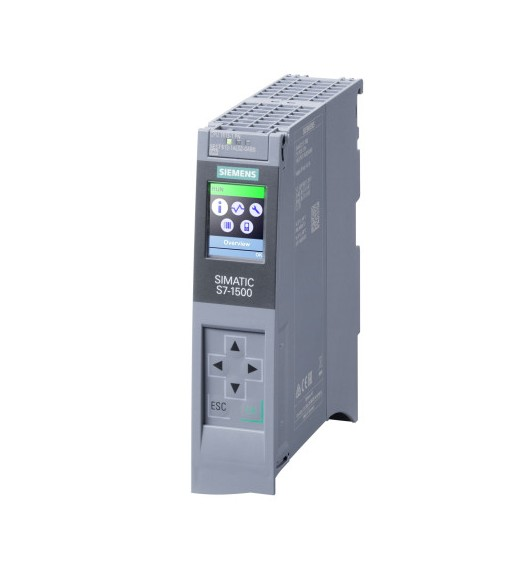
\includegraphics[width=0.3\textwidth]{PLC Siemens S7 1500}
    \caption{PLC industrial Siemens SIMATIC S7-1500, CPU 1513-1~PN~\cite{ref17}.}
    \label{fig:ctrl_s71500}
\end{figure}

\textbf{Alternativa 2: sistema didáctico Festo EduTrainer Universal con SIMATIC S7-1500.} Banco de laboratorio que integra un PLC Siemens de la misma familia sobre un bastidor con los bornes de seguridad de 4~mm, los interruptores de simulación de entradas y los pilotos de salida ya cableados y protegidos contra cortocircuito~\cite{ref18}. Su ventaja es que llega listo para el laboratorio, con las señales del PLC accesibles y protegidas. Sus desventajas frente al objetivo del proyecto son tres: es un formato de banco cerrado, que no permite reorganizar el montaje ni incorporar módulos distintos para adaptar la plataforma a prácticas nuevas; conserva la dependencia del entorno TIA~Portal y de su licencia; y atiende un único puesto de trabajo por unidad, cuyo precio de mercado equivale al de un PLC industrial completo, de modo que equipar el laboratorio resulta tan oneroso como con la Alternativa 1, con independencia de que la Escuela ya disponga de una unidad. La Figura~\ref{fig:ctrl_edutrainer} muestra el conjunto.

\begin{figure}[H]
    \centering
    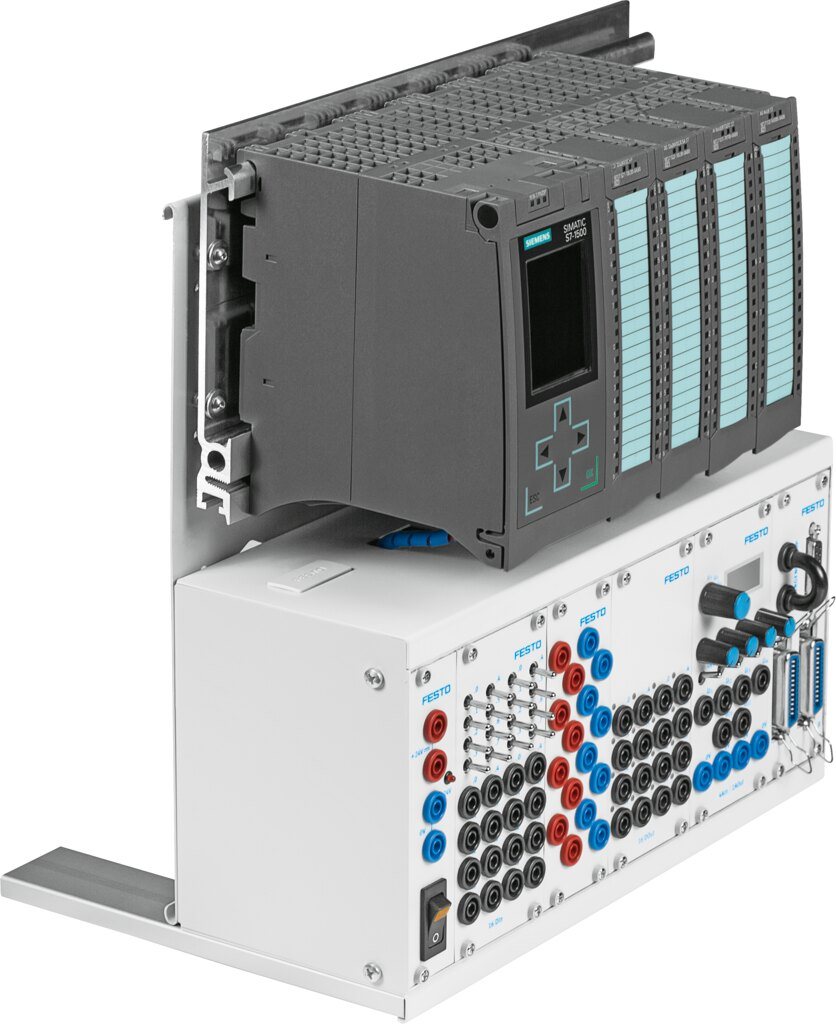
\includegraphics[width=0.22\textwidth]{Edu_trainer}
    \caption{Sistema didáctico Festo EduTrainer Universal con PLC SIMATIC S7-1500~\cite{ref18}.}
    \label{fig:ctrl_edutrainer}
\end{figure}

\textbf{Alternativa 3: placa de microcontrolador de propósito general Arduino UNO R3.} Placa basada en el microcontrolador ATmega328P, con entradas y salidas digitales a 5~V y seis entradas analógicas~\cite{ref19}. Es la alternativa de menor costo (19{,}95~USD~\cite{ref19}) y la de mayor disponibilidad en el mercado nacional. No obstante, no maneja señales industriales a 24~V sin electrónica de adaptación externa, no dispone de salidas de relé ni de formato de montaje en riel DIN y no se programa con los lenguajes normados por IEC~61131-3, sino en C/C++; la competencia que el estudiante adquiriría no sería directamente transferible al entorno industrial. La Figura~\ref{fig:ctrl_uno} muestra la placa.

\begin{figure}[H]
    \centering
    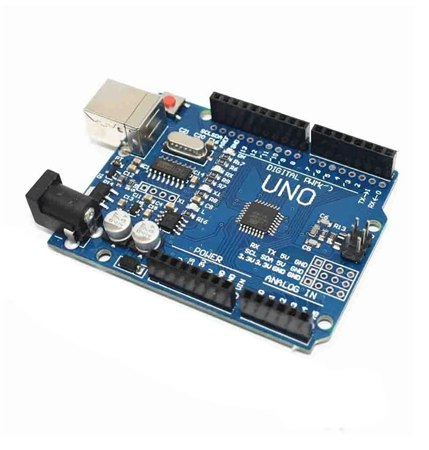
\includegraphics[width=0.3\textwidth]{Arduino_UNO_R3_red}
    \caption{Placa Arduino UNO R3~\cite{ref19}.}
    \label{fig:ctrl_uno}
\end{figure}

\textbf{Alternativa 4: placa de microcontrolador con conectividad inalámbrica ESP32.} Placa de desarrollo basada en el módulo ESP-WROOM-32, con WiFi y Bluetooth integrados y un costo de 15{,}95~USD~\cite{ref20}. Añade la conectividad de red que el UNO no trae, pero comparte con él todas las limitaciones frente al objetivo del proyecto: entradas y salidas a 3{,}3~V, ausencia de manejo nativo de 24~V, de salidas de relé y de formato DIN, y programación fuera del marco de IEC~61131-3. La Figura~\ref{fig:ctrl_esp32} muestra la placa.

\begin{figure}[H]
    \centering
    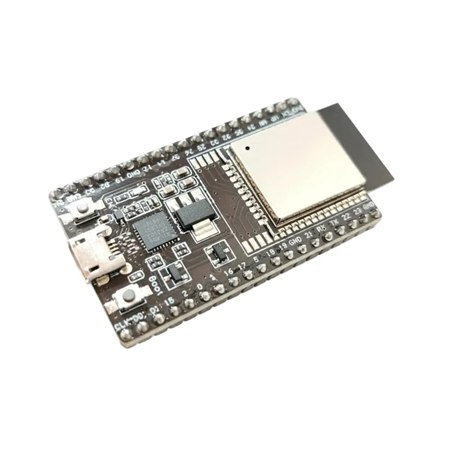
\includegraphics[width=0.3\textwidth]{esp32_red}
    \caption{Placa de desarrollo ESP32~\cite{ref20}.}
    \label{fig:ctrl_esp32}
\end{figure}

\textbf{Alternativa 5: micro-PLC de orientación industrial Arduino Opta WiFi.} Controlador de grado industrial en formato de montaje en riel DIN, con ocho entradas de 0 a 24~V~DC para contactos secos y sensores PNP, cuatro salidas de relé de contacto seco, puerto AUX para encadenar módulos de expansión y programación en Ladder Diagram, Function Block Diagram y Structured Text desde el entorno gratuito Arduino PLC IDE~\cite{ref1,ref8}. Sus especificaciones completas, sus módulos de expansión y el análisis de su accesibilidad económica se presentan en la Sección~\ref{sec:opta}, cuya Figura~\ref{fig:opta_estetico} muestra el equipo. Es la alternativa seleccionada.

% -------------------------------------------------
\subsection{Alternativas de material estructural consideradas}
% -------------------------------------------------

La segunda decisión de selección corresponde al material con que se construye la estructura de soporte. Se plantearon cinco alternativas, identificadas mediante investigación bibliográfica sobre estructuras de bancos didácticos y revisión de la oferta de los proveedores nacionales consultados. Los criterios de evaluación se derivan directamente de los requerimientos enumerados en la Sección~\ref{subsec:requerimientos}:

\begin{itemize}
    \item \textbf{Rigidez y relación resistencia-peso:} capacidad del material de sostener el panel de acrílico y el conjunto de módulos montados sin deformación apreciable, ponderada contra la masa total resultante del conjunto.
    \item \textbf{Modularidad y reconfigurabilidad:} posibilidad de reubicar, agregar o retirar elementos sin practicar perforaciones nuevas ni comprometer la integridad del material.
    \item \textbf{Facilidad de fabricación y ensamble:} grado en que el material puede cortarse, unirse y montarse con los recursos y las herramientas efectivamente disponibles en el Campus.
    \item \textbf{Costo y disponibilidad local:} costo del material para la geometría requerida y plazo de entrega de los proveedores nacionales consultados.
    \item \textbf{Acabado, seguridad y presentación:} calidad del acabado superficial, ausencia de bordes cortantes expuestos y adecuación estética a un equipo de uso docente.
\end{itemize}

\textbf{Alternativa 1: perfil de aluminio ranurado tipo T-slot.} Perfil extruido de aluminio de sección cuadrada con ranura longitudinal en sus cuatro caras, unido mediante tuercas T y tornillería métrica. Su rasgo distintivo es que la ranura permite fijar un elemento en cualquier punto del perfil sin perforar, lo que convierte a la estructura en reconfigurable por diseño. Es un material normalizado, disponible en el mercado nacional y de bajo peso específico.

\textbf{Alternativa 2: madera o tablero de MDF.} Estructura construida a partir de tableros cortados y unidos con tornillería o adhesivo. Es la opción de menor costo por unidad de superficie y la más sencilla de trabajar con herramienta manual. En contrapartida, no ofrece ningún mecanismo de fijación reconfigurable, por lo que toda modificación posterior exige perforar nuevamente el tablero, lo que degrada progresivamente el material. Además, es sensible a la humedad y su acabado tiende a deteriorarse con la manipulación repetida.

\textbf{Alternativa 3: lámina o ángulo de acero.} Estructura de perfilería de acero unida por soldadura o por tornillería pasante. Es la alternativa de mayor rigidez y la más económica si se valora por unidad de masa. Sin embargo, requiere soldadura o taladrado para cada unión, operaciones que no están disponibles de forma inmediata en el Campus; incrementa considerablemente el peso del conjunto, lo que dificulta el transporte entre aulas; y exige un tratamiento superficial adicional para evitar bordes cortantes y corrosión.

\textbf{Alternativa 4: estructura completamente impresa en 3D.} Fabricación de la totalidad de los elementos estructurales en las impresoras 3D disponibles, que son exclusivamente de marca Creality. Ofrece libertad geométrica total y no depende de proveedores externos, pero su viabilidad quedó acotada por dos limitaciones. La primera es la dureza del material, porque el plástico impreso no alcanza la rigidez y dureza necesarias para sostener el panel cargado sin deformación apreciable, y su resistencia disminuye en la dirección de las capas de impresión. La segunda es el tamaño de las piezas, pues los tramos rectos de 500~mm exceden el volumen de trabajo de las impresoras 3D disponibles, de modo que la alternativa exigiría máquinas de formato mayor que no se tienen. Fabricarla con las impresoras existentes obligaría a seccionar cada tramo, imprimirlo por partes y unirlas, con la consiguiente pérdida de rigidez en cada junta y con tiempos de impresión acumulados elevados.

\textbf{Alternativa 5: tubo o perfil estructural de PVC.} Estructura de tubería plástica unida mediante accesorios encolados. Es liviana y económica, y se consigue con facilidad en el mercado local. Sus limitaciones son la baja rigidez frente a cargas de flexión, la escasa precisión dimensional de las uniones encoladas, que impide garantizar la perpendicularidad y el ángulo de inclinación requeridos por el diseño, y la ausencia de todo mecanismo de fijación reconfigurable, de modo que montar o reubicar un módulo obliga a practicar agujeros nuevos sobre el tubo, y como los accesorios van encolados de forma permanente, cualquier cambio en la geometría exige cortar y rehacer la unión en lugar de simplemente aflojarla.

% -------------------------------------------------
\subsection{Alternativas de interfaz de acoplamiento consideradas}
% -------------------------------------------------

La tercera decisión de selección del proyecto corresponde a la etapa de acoplamiento entre el dominio industrial de 24~V~DC y los circuitos de baja tensión que el estudiante construye en los demás laboratorios de la carrera (habitualmente a 5~V, pero con la tensión que cada diseño requiera), cuya necesidad se fundamentó en la Sección~\ref{subsec:optoacoplador}. Se evaluaron tres alternativas disponibles en el proveedor nacional consultado.

\textbf{Alternativa 1: optoacoplador 4N25 en encapsulado DIP-6.} Componente individual que integra un diodo emisor de infrarrojo y un fototransistor NPN en un encapsulado de seis pines, con una tensión de aislamiento de 5\,300~V~rms~\cite{ref16}. Es la opción de menor costo unitario y la de mayor tensión de aislamiento de las tres. Su limitación no es eléctrica sino de integración, ya que, al tratarse de un chip suelto, incorporarlo exige diseñar y fabricar una placa que aloje el componente, las resistencias limitadoras de cada lado y las borneras de conexión, además de resolver su sujeción sobre el panel. Ese trabajo adicional de montaje y adaptación no aporta ninguna prestación que las alternativas en placa no ofrezcan ya resueltas. La Figura~\ref{fig:opto_4n25} muestra el componente.

\begin{figure}[H]
    \centering
    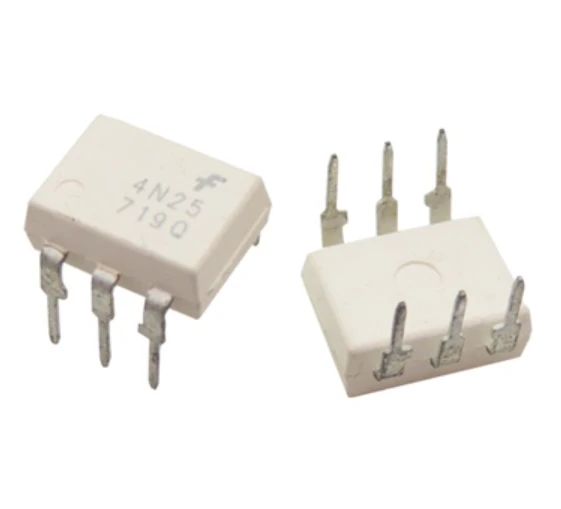
\includegraphics[width=0.3\textwidth]{Optoacoplador_4N25.png}
    \caption{Optoacoplador 4N25 en encapsulado DIP-6~\cite{ref16}.}
    \label{fig:opto_4n25}
\end{figure}

\textbf{Alternativa 2: módulo controlador de MOSFET con aislamiento óptico.} Placa ensamblada que combina un optoacoplador con un MOSFET de canal N en encapsulado TO-220, con entrada de 3 a 20~V, salida de 5 a 36~V y capacidad de hasta 10~A, admitiendo señal PWM de hasta 20~kHz~\cite{ref15}. Está concebida como etapa de potencia para gobernar motores, lámparas o electroválvulas, no como interfaz de señal. Para el uso previsto resulta sobredimensionada en corriente y, sobre todo, ofrece un solo canal a un costo superior al de la alternativa de cuatro canales, lo que la vuelve la opción menos eficiente en términos de canales disponibles por unidad de costo. En la Figura~\ref{fig:opto_mosfet} se aprecia la placa, con el MOSFET en encapsulado TO-220 y las borneras de entrada y de salida.

\begin{figure}[H]
    \centering
    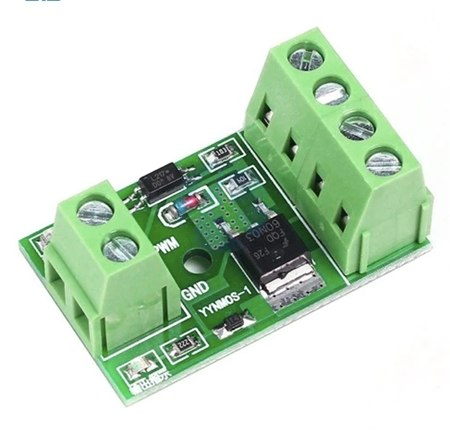
\includegraphics[width=0.3\textwidth]{Optoacoplador_MOSFET_red}
    \caption{Módulo controlador de MOSFET con aislamiento óptico~\cite{ref15}.}
    \label{fig:opto_mosfet}
\end{figure}

\textbf{Alternativa 3: tarjeta optoacopladora de cuatro canales basada en el PC817.} Placa ensamblada con cuatro optoacopladores PC817 independientes, borneras atornillables en ambos lados, puentes de configuración de tierra por canal y cuatro perforaciones de sujeción. Admite señales de entrada entre 3,6 y 24~V y gobierna salidas entre 3,6 y 30~V~\cite{ref13}, y cada PC817 aporta una tensión de aislamiento de 5\,000~V~rms con una CTR mínima del 50~\%~\cite{ref14}. Cubre por tanto de forma directa, sin electrónica intermedia, el nivel del controlador en la entrada y, en la salida, cualquier tensión de alimentación del circuito del estudiante dentro de ese rango. La Figura~\ref{fig:opto_pc817} muestra la disposición de los cuatro canales, con sus borneras y sus puentes de configuración.

\begin{figure}[H]
    \centering
    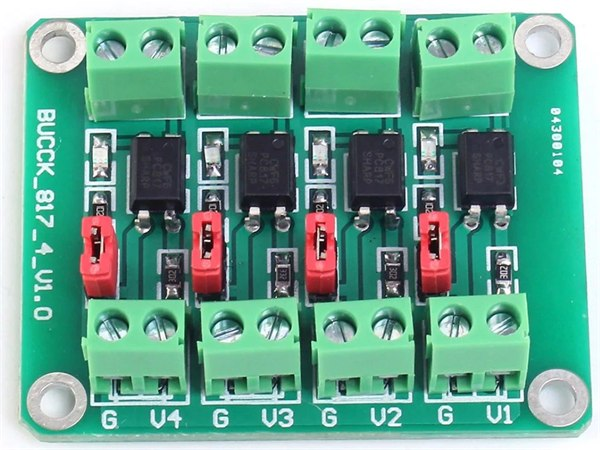
\includegraphics[width=0.4\textwidth]{Optoacoplador_PC817_red}
    \caption{Tarjeta optoacopladora de cuatro canales basada en el PC817~\cite{ref13}.}
    \label{fig:opto_pc817}
\end{figure}

% -------------------------------------------------
\subsection{Alternativas de sensor de proximidad consideradas}
\label{subsec:alternativas_sensor}
% -------------------------------------------------

Además de las tres decisiones que definen la arquitectura de la plataforma, el equipo se complementa con los dispositivos de campo que el estudiante conecta a las borneras para ejercitar las entradas y salidas del controlador: un sensor de proximidad de detección sin contacto como entrada representativa del entorno industrial, un juego de botones que aportan entradas de mando accionadas por el operador y un juego de luces indicadoras como cargas de salida. Aquí se plantean las alternativas de sensor de proximidad y su selección mediante matriz de Pugh se presenta en la Sección~\ref{subsec:seleccion_sensor}. Los botones y las luces no se sometieron a una matriz de Pugh, porque no constituyen una decisión con alternativas tecnológicas que ponderar sino elementos auxiliares de catálogo; se eligieron por su compatibilidad con el dominio de 24~V~DC de la plataforma, su conexión directa a las borneras sin soldadura y una cantidad suficiente para una práctica con varias señales. Los dispositivos seleccionados se describen en la Sección~\ref{subsec:hw_campo}.

Los criterios de evaluación se derivan del objetivo docente de que el sensor enfrente al estudiante con el caso de detección más habitual en la automatización industrial, que se conecte directamente a las entradas del Opta sin electrónica intermedia, que opere de forma fiable en un aula sin condiciones ambientales controladas y que esté disponible en el mercado a bajo costo. Las entradas digitales del Opta están concebidas para dispositivos de contacto seco y para sensores de tipo PNP (a tres hilos, con salida en colector abierto a $+$24~V), que entregan el nivel activo directamente a la entrada sin necesidad de resistencias externas~\cite{ref8}; los sensores con salida NPN, en cambio, exigen una resistencia de polarización externa hacia $+$24~V para que la entrada reconozca el estado activo. Se compararon tres sensores de proximidad ofrecidos por los proveedores consultados: dos de tecnología inductiva (uno cilíndrico con salida PNP y uno rectangular con salida NPN) y uno de tecnología capacitiva con salida PNP.

\textbf{Alternativa 1: sensor de proximidad inductivo LJ12A3-4-Z/BY.} Sensor cilíndrico con rosca M12 que detecta la presencia de objetos metálicos por la pérdida que inducen las corrientes de Foucault en el campo magnético de alta frecuencia generado en su cara activa~\cite{ref23}. Tiene una distancia de detección de 4~mm~$\pm$~10~\%, alimentación de 6 a 36~V~DC, salida PNP normalmente abierta a tres hilos con capacidad de 300~mA y grado de protección IP67~\cite{ref21}. Solo detecta metales (con el mayor alcance sobre materiales ferrosos) y es insensible a la presencia de polvo, humedad o variaciones de temperatura~\cite{ref23}. Su precio de venta al público se sitúa entre 8 y 13~USD según la oferta del mercado en línea~\cite{ref21}. La Figura~\ref{fig:sensor_inductivo} muestra el dispositivo.

\begin{figure}[H]
    \centering
    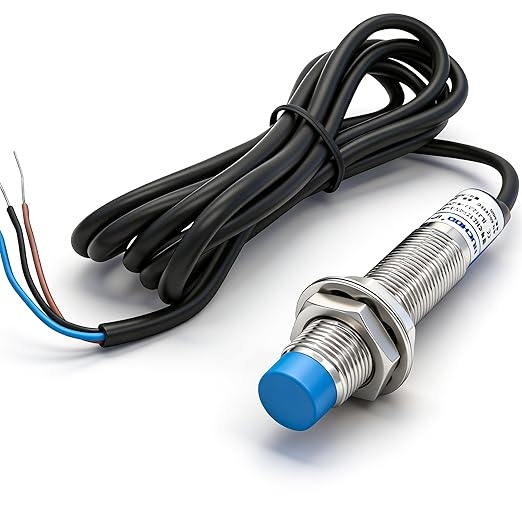
\includegraphics[width=0.3\textwidth]{Sensor_proximidad_inductivo}
    \caption{Sensor de proximidad inductivo LJ12A3-4-Z/BY, variante PNP normalmente abierta~\cite{ref21}.}
    \label{fig:sensor_inductivo}
\end{figure}

\textbf{Alternativa 2: sensor de proximidad inductivo rectangular SN04-N.} Sensor inductivo de cuerpo rectangular (36$\times$18$\times$18~mm) en carcasa de resina, con dos orificios para tornillo M3 que permiten fijarlo en plano sobre una superficie sin tuercas ni soporte adicional. Detecta objetos metálicos por el mismo principio que la Alternativa~1, con una distancia de detección de 4~mm, alimentación de 10 a 30~V~DC, salida a tres hilos con capacidad cercana a 300~mA y grado de protección IP67~\cite{ref24}. Es el más económico de los tres (5,95~USD~\cite{ref24}) y su forma facilita fijarlo sobre una superficie plana, pero solo se ofrece con salida NPN; para que la entrada del Opta lea el nivel activo hay que intercalar una resistencia de polarización externa hacia $+$24~V, un cableado adicional que el estudiante debe realizar correctamente. En el proveedor nacional consultado figura además sin existencias. La Figura~\ref{fig:sensor_sn04n} muestra el dispositivo.

\begin{figure}[H]
    \centering
    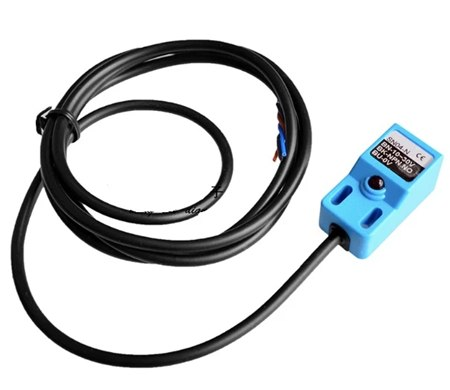
\includegraphics[width=0.3\textwidth]{Sensor_proximidad_SN04N_red}
    \caption{Sensor de proximidad inductivo rectangular SN04-N, salida NPN normalmente abierta~\cite{ref24}.}
    \label{fig:sensor_sn04n}
\end{figure}

\textbf{Alternativa 3: sensor de proximidad capacitivo LJC18A3-B-Z/BY.} Sensor cilíndrico con rosca M18 que detecta la presencia de un objeto por la variación de capacitancia entre su electrodo sensor y el blanco, mecanismo que responde tanto a metales como a materiales no metálicos (plásticos, madera, vidrio, líquidos y sólidos granulados)~\cite{ref23}. Tiene una distancia de detección ajustable mediante un potenciómetro hasta unos 10~mm, alimentación de 6 a 36~V~DC, salida PNP normalmente abierta a tres hilos con capacidad de 300~mA y grado de protección IP67~\cite{ref22}. Su ventaja es la variedad de materiales que reconoce; sus desventajas para el uso previsto son la mayor sensibilidad a la humedad, el polvo y la temperatura ambiente, la necesidad de calibrar la sensibilidad para cada aplicación y la propensión a disparos falsos ante objetos cercanos o la mano del estudiante~\cite{ref23}. Su precio de venta al público se sitúa entre 10 y 14~USD según la oferta del mercado en línea~\cite{ref22}. La Figura~\ref{fig:sensor_capacitivo} muestra el dispositivo.

\begin{figure}[H]
    \centering
    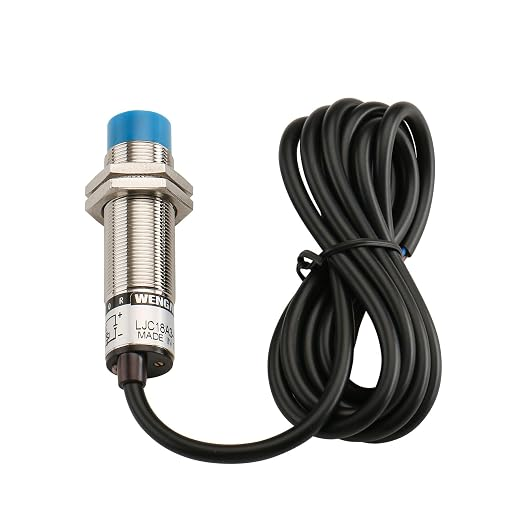
\includegraphics[width=0.3\textwidth]{Sensor_proximidad_capacitivo}
    \caption{Sensor de proximidad capacitivo LJC18A3-B-Z/BY, variante PNP normalmente abierta~\cite{ref22}.}
    \label{fig:sensor_capacitivo}
\end{figure}

% -------------------------------------------------
\section{Implementación de la solución}
\label{sec:implementacion}
% -------------------------------------------------

Definida la alternativa estructural, la implementación se ejecutó en cuatro pasos: optimización de la geometría y definición del plan de corte, diseño de las piezas de unión no normalizadas, verificación del ensamble mediante modelado 3D en Autodesk Fusion~360 y montaje físico de la estructura. El criterio que guió la geometría fue reducir el número de perfiles conservando la estabilidad del conjunto y el ángulo de presentación del panel, y el modelado previo permitió confirmar las dimensiones antes de realizar cortes irreversibles sobre la perfilería adquirida. Como el resultado de estos pasos es parte de la solución y no una alternativa evaluada, el plan de corte, las piezas de unión, el modelo de ensamble y el montaje se describen en la Sección~\ref{subsec:hw_estructura}.

% -------------------------------------------------
\section{Reevaluación y rediseño}
% -------------------------------------------------

La estructura ensamblada se sometió a una revisión de estabilidad y de acceso, en la que se verificó que el conjunto se apoyara sin balanceo, que el ángulo de 70° permitiera la lectura de los indicadores y la manipulación de las borneras, y que ninguna arista o cabeza de tornillo expuesta pudiera causar alguna lesión. Los criterios que se sugiere aplicar para determinar mejoras futuras sobre esta estructura son la aparición de deformación permanente o daño en las piezas de PLA tras un uso prolongado, en cuyo caso la pieza afectada debe reemplazarse por la misma pieza de unión impresa en ABS, un material de mayor resistencia mecánica y confiabilidad; la necesidad de ampliar el número de módulos montados sobre el panel, que se resolvería aprovechando la ranura del perfil sin rediseñar la estructura; y la conveniencia de incorporar elementos de sujeción para el transporte del equipo entre aulas.



% =================================================================
\chapter{Descripción detallada de la solución}
\label{chp:enfoque}
% =================================================================

Mientras que el Capítulo~\ref{chp:procedimientos} documenta el procedimiento seguido (cómo se reconoció el problema, qué información lo acotó y qué alternativas se plantearon y con qué método se compararon), este capítulo presenta la selección de la alternativa en cada decisión y el diseño de la solución implementada. Se presentan primero las matrices de Pugh y las alternativas seleccionadas; luego la estructura, el funcionamiento de cada módulo de hardware y los dispositivos de campo; y por último el software que gobierna la plataforma; el capítulo cierra con el análisis costo-beneficio frente a los PLC industriales convencionales. La exposición sigue el orden en que el sistema se implementó.

La solución consiste en una plataforma didáctica modular que separa físicamente el núcleo de control de las interfaces de experimentación. Esta arquitectura de dos niveles responde directamente a las limitaciones identificadas en el estado del arte, ya que protege el hardware de control de la manipulación directa de los estudiantes, permite adaptar el sistema a distintos escenarios sin reconfigurar el cableado principal y reduce el costo por estudiante al hacer reutilizable la inversión en la plataforma base. El enfoque es análogo al principio de separación entre gabinete de control y tablero de campo utilizado en instalaciones industriales reales, lo que le añade valor formativo más allá de la práctica de programación, porque el estudiante interioriza desde el inicio de su formación la lógica de protección, identificación y segmentación de sistemas de control.

La plataforma no replica de forma directa ninguno de los enfoques documentados en el estado del arte. A diferencia de los kits comerciales, está diseñada para el contexto institucional del Campus San Carlos, con componentes disponibles comercialmente, documentación técnica abierta y una estructura modular que puede crecer conforme evoluciona el plan de estudios. A diferencia de los laboratorios modulares reportados en la literatura, incorpora desde el diseño la protección del hardware de control como condición de operación y no como restricción administrativa. Su software de programación es de acceso gratuito, por lo que el programa puede replicar, mantener y ampliar el sistema con recursos propios.

% -------------------------------------------------
\section{Análisis de soluciones y selección final}
\label{sec:analisis_soluciones}
% -------------------------------------------------

Las alternativas consideradas para cada decisión de diseño y el método de comparación se documentaron en la Sección~\ref{subsec:escala} y siguientes del Capítulo~\ref{chp:procedimientos}. Esta sección presenta la matriz de Pugh de cada decisión y la alternativa seleccionada: la unidad de control que gobierna el sistema, el material de la estructura de soporte, la interfaz que acopla los 24~V~DC con los circuitos de baja tensión del estudiante y, como decisión complementaria, el sensor de proximidad. La unidad de control se presenta primero porque condiciona a las otras decisiones.

% -------------------------------------------------
\subsection{Selección de la unidad de control}
\label{subsec:seleccion_unidad}
% -------------------------------------------------

La Tabla~\ref{tab:comparacion_unidad_control} presenta la matriz de Pugh de las cinco alternativas. Los tres criterios de mayor peso son la compatibilidad con IEC~61131-3 y la operación nativa con señales de 24~V (las condiciones que hacen transferible la competencia al entorno industrial) y el costo de adquisición y replicabilidad, decisivo en un laboratorio que debe equiparse con varias unidades; los demás criterios completan la evaluación con pesos menores.

\begin{table}[H]
\centering
\caption{Matriz de Pugh. Selección de la unidad de control. Fuente: Autora.}
\label{tab:comparacion_unidad_control}
\footnotesize
\setlength{\tabcolsep}{4pt}
\renewcommand{\arraystretch}{1.3}
\renewcommand\tabularxcolumn[1]{m{#1}}
\begin{tabularx}{\textwidth}{|>{\raggedright\arraybackslash}m{3.9cm}|>{\centering\arraybackslash}p{0.8cm}|*{5}{>{\centering\arraybackslash}X|}}
\hline
\filacolor{TableGray}
\textbf{Criterio} & \textbf{Peso} & \textbf{Siemens S7-1500} & \textbf{Festo Edu\-Trainer} & \textbf{Arduino UNO R3} & \textbf{ESP32} & \textbf{Arduino Opta WiFi} \\
\hline
Compatibilidad con IEC 61131-3 (LD, FBD, ST) & 0,20 & 5 & 5 & 1 & 1 & 5 \\
\hline
Operación nativa con señales industriales a 24 V & 0,17 & 4 & 5 & 1 & 1 & 5 \\
\hline
Costo de adquisición y replicabilidad para el laboratorio & 0,18 & 1 & 1 & 5 & 5 & 4 \\
\hline
Entorno de programación de acceso gratuito & 0,11 & 2 & 2 & 5 & 5 & 5 \\
\hline
Formato de montaje e integración en un panel reconfigurable & 0,12 & 2 & 2 & 3 & 3 & 5 \\
\hline
Expansión modular de entradas y salidas & 0,08 & 5 & 2 & 2 & 2 & 4 \\
\hline
Disponibilidad y soporte en el mercado local & 0,06 & 3 & 3 & 5 & 4 & 3 \\
\hline
Robustez para entorno industrial (protección, rango térmico) & 0,08 & 5 & 5 & 2 & 2 & 5 \\
\hline
\filacolor{TableGray}
\textbf{Puntaje ponderado (1--5)} & \textbf{1,00} & \textbf{3,30} & \textbf{3,23} & \textbf{2,80} & \textbf{2,74} & \textbf{4,62} \\
\hline
\end{tabularx}
\end{table}

El Arduino Opta WiFi obtuvo el puntaje ponderado más alto (4{,}62) y es la alternativa seleccionada. El PLC industrial Siemens S7-1500 (3{,}30) y el Festo EduTrainer (3{,}23) reciben buenas calificaciones en fidelidad industrial, compatibilidad con IEC~61131-3 y robustez, pero quedan penalizados por el costo de adquisición y de licenciamiento (solo la CPU del S7-1500 cuesta 1.746{,}51~EUR~\cite{ref17}, más del doble que el kit completo del Opta, sin contar los módulos de E/S ni la licencia de TIA~Portal) y por su formato, que no se integra en el panel reconfigurable del proyecto; el EduTrainer, además, es un banco cerrado que atiende un solo puesto por unidad. Las placas Arduino UNO R3 (2{,}80) y ESP32 (2{,}74) obtienen los puntajes más bajos porque, pese a su costo mínimo y su disponibilidad local, no operan con señales industriales a 24~V sin electrónica de adaptación y no se programan con los lenguajes de IEC~61131-3, con lo que la competencia adquirida no sería transferible al entorno industrial.

El Arduino Opta WiFi es la única alternativa que combina las tres condiciones que el proyecto no podía ceder (programación en los lenguajes de IEC~61131-3, operación nativa a 24~V~DC y un costo que hace viable replicar varias unidades), lo que explica su ventaja en el puntaje ponderado. La calificación del EduTrainer en el criterio de costo se asignó equivalente a la del S7-1500, porque su precio de mercado es comparable~\cite{ref47}, por integrar un PLC de la misma familia sobre un bastidor instrumentado, y disponer de una unidad en la Escuela no reduce el costo de replicarlo para todos los puestos del laboratorio. Las demás implicaciones de la elección del Opta (especificaciones, módulos de expansión y accesibilidad económica) se retoman en la Sección~\ref{sec:opta}.

% -------------------------------------------------
\subsection{Selección de la alternativa estructural}
\label{subsec:seleccion_material}
% -------------------------------------------------

La Tabla~\ref{tab:comparacion_materiales} presenta la matriz de Pugh de las cinco alternativas frente a los cinco criterios definidos. La modularidad y la facilidad de fabricación reciben los pesos más altos por ser los dos requerimientos que el proyecto no puede ceder, ya que son los que permiten que la plataforma se adapte a prácticas distintas a lo largo del tiempo y que sus piezas no normalizadas puedan producirse con los equipos del Campus.

\begin{table}[H]
\centering
\caption{Matriz de Pugh. Selección del material estructural. Fuente: Autora.}
\label{tab:comparacion_materiales}
\footnotesize
\setlength{\tabcolsep}{4pt}
\renewcommand{\arraystretch}{1.3}
\renewcommand\tabularxcolumn[1]{m{#1}}
\begin{tabularx}{\textwidth}{|>{\raggedright\arraybackslash}m{4.2cm}|>{\centering\arraybackslash}p{0.8cm}|*{5}{>{\centering\arraybackslash}X|}}
\hline
\filacolor{TableGray}
\textbf{Criterio} & \textbf{Peso} & \textbf{Perfil Al. T-slot} & \textbf{Madera / MDF} & \textbf{Acero} & \textbf{Impresión 3D} & \textbf{PVC} \\
\hline
Rigidez y relación resistencia-peso & 0,18 & 5 & 3 & 3 & 2 & 2 \\
\hline
Modularidad y reconfigurabilidad & 0,28 & 5 & 2 & 2 & 3 & 1 \\
\hline
Facilidad de fabricación y ensamble con recursos del Campus & 0,24 & 5 & 4 & 2 & 3 & 3 \\
\hline
Costo y disponibilidad local & 0,15 & 3 & 5 & 4 & 4 & 5 \\
\hline
Acabado, seguridad y presentación & 0,15 & 5 & 3 & 2 & 3 & 3 \\
\hline
\filacolor{TableGray}
\textbf{Puntaje ponderado (1--5)} & \textbf{1,00} & \textbf{4,70} & \textbf{3,26} & \textbf{2,48} & \textbf{2,97} & \textbf{2,56} \\
\hline
\end{tabularx}
\end{table}

El perfil de aluminio ranurado tipo T-slot obtuvo el puntaje ponderado más alto (4{,}70) y es la alternativa seleccionada. Es la única que satisface simultáneamente los dos criterios de mayor peso: la modularidad (la ranura permite fijar o reubicar un elemento en cualquier punto sin perforar) y la facilidad de fabricación con los recursos del Campus. La madera (3{,}26) y el PVC (2{,}56) reciben buenas calificaciones en costo, pero quedan penalizados por carecer de un mecanismo de fijación reconfigurable, condición que es precisamente lo que permite que la plataforma se adapte a prácticas distintas a lo largo del tiempo. El acero (2{,}48) es el material más rígido en términos absolutos, pero su densidad eleva la masa del conjunto hasta comprometer el requerimiento de transporte entre aulas y exige operaciones de soldadura no disponibles en el Campus, por lo que obtiene solo 3 puntos en la relación resistencia-peso y 2 en facilidad de fabricación. La impresión 3D integral (2{,}97) permite incorporar las geometrías de fijación en la propia pieza, pero cada modificación posterior obliga a reimprimir el elemento completo, y los tramos de 500~mm exceden el volumen de trabajo de las impresoras disponibles.

El costo unitario del perfil de aluminio es superior al de la madera y al del PVC, pero ese sobrecosto queda acotado por el propio diseño, porque la geometría se optimizó hasta requerir únicamente seis perfiles, como se explica en la Sección~\ref{subsec:hw_estructura}, y el monto total de la perfilería asciende a ₡30.358{,}77 según la cotización CB2026050402 de CRCibernética, cifra plenamente compatible con el presupuesto del proyecto. Se seleccionó por tanto el perfil de aluminio T-slot de sección 20$\times$20~mm en tramos de 500~mm, complementado con piezas de unión de diseño propio, fabricadas por impresión 3D, para resolver las uniones que la tornillería normalizada no cubre.

% -------------------------------------------------
\subsection{Selección de la interfaz de acoplamiento}
\label{subsec:seleccion_opto}
% -------------------------------------------------

La Tabla~\ref{tab:comparacion_optoacopladores} presenta la matriz de Pugh de las tres alternativas. La idoneidad funcional (que el dispositivo sea una interfaz de señal y no una etapa de potencia) y la cobertura directa de los 24~V del controlador y de la tensión del circuito del estudiante (5~V como caso habitual) reciben los pesos más altos, por definir si la alternativa resuelve el problema planteado sin electrónica intermedia.

\begin{table}[H]
\centering
\caption{Matriz de Pugh. Selección de la interfaz de acoplamiento. Fuente: Autora.}
\label{tab:comparacion_optoacopladores}
\footnotesize
\setlength{\tabcolsep}{4pt}
\renewcommand{\arraystretch}{1.3}
\renewcommand\tabularxcolumn[1]{m{#1}}
\begin{tabularx}{\textwidth}{|>{\raggedright\arraybackslash}m{5.2cm}|>{\centering\arraybackslash}p{0.9cm}|*{3}{>{\centering\arraybackslash}X|}}
\hline
\filacolor{TableGray}
\textbf{Criterio} & \textbf{Peso} & \textbf{4N25 DIP-6} & \textbf{Módulo MOSFET} & \textbf{Tarjeta PC817} \\
\hline
Idoneidad funcional como interfaz de señal & 0,24 & 4 & 2 & 5 \\
\hline
Cobertura directa de 24 V y de la tensión del circuito del estudiante sin electrónica intermedia & 0,20 & 2 & 4 & 5 \\
\hline
Integración al panel sin fabricación adicional & 0,18 & 1 & 5 & 5 \\
\hline
Canales disponibles por unidad & 0,16 & 1 & 1 & 5 \\
\hline
Costo por canal & 0,12 & 5 & 1 & 4 \\
\hline
Tensión de aislamiento & 0,10 & 5 & 2 & 5 \\
\hline
\filacolor{TableGray}
\textbf{Puntaje ponderado (1--5)} & \textbf{1,00} & \textbf{2,80} & \textbf{2,66} & \textbf{4,88} \\
\hline
\end{tabularx}
\end{table}

La tarjeta optoacopladora de cuatro canales basada en el PC817 obtuvo el puntaje ponderado más alto (4{,}88) y es la alternativa seleccionada. Resuelve simultáneamente los criterios de mayor peso, pues sus rangos de tensión cubren de forma directa el acoplamiento entre los 24~V del controlador y cualquier tensión de 3,6 a 30~V del lado del estudiante, es una interfaz de señal y no una etapa de potencia, y al venir ensamblada y con perforaciones de sujeción se integra al panel sin fabricación adicional; sus cuatro canales permiten además que el estudiante gobierne varios circuitos en una misma práctica sin ampliar el montaje. El optoacoplador 4N25 (2{,}80) es el más económico por canal y el de mayor tensión de aislamiento, pero como componente suelto obliga a diseñar y fabricar una placa que aloje el chip, las resistencias limitadoras y las borneras, un trabajo que no aporta prestaciones adicionales e introduce un punto de falla propio en un equipo destinado a uso estudiantil. El módulo controlador de MOSFET (2{,}66) queda penalizado por corresponder a una función distinta de la requerida (es una etapa de potencia y no una interfaz de señal) y por entregar un único canal a un costo mayor que el de la tarjeta de cuatro.

% -------------------------------------------------
\subsection{Selección del sensor de proximidad}
\label{subsec:seleccion_sensor}
% -------------------------------------------------

La Tabla~\ref{tab:comparacion_sensor_proximidad} presenta la matriz de Pugh de las tres alternativas, con la escala de la Tabla~\ref{tab:criterios_calificacion}. La representatividad del caso de detección industrial más común, la inmunidad a las condiciones ambientales de un aula y la conexión directa a las entradas del Opta reciben los pesos más altos, por ser los factores que determinan el valor formativo del sensor y la fiabilidad de las prácticas.

\begin{table}[H]
\centering
\caption{Matriz de Pugh. Selección del sensor de proximidad. Fuente: Autora.}
\label{tab:comparacion_sensor_proximidad}
\footnotesize
\setlength{\tabcolsep}{4pt}
\renewcommand{\arraystretch}{1.3}
\renewcommand\tabularxcolumn[1]{m{#1}}
\begin{tabularx}{\textwidth}{|>{\raggedright\arraybackslash}m{5.2cm}|>{\centering\arraybackslash}p{0.9cm}|*{3}{>{\centering\arraybackslash}X|}}
\hline
\filacolor{TableGray}
\textbf{Criterio} & \textbf{Peso} & \textbf{Inductivo PNP (LJ12A3)} & \textbf{Inductivo NPN (SN04-N)} & \textbf{Capacitivo PNP (LJC18A3)} \\
\hline
Representatividad del caso de detección más común en la industria & 0,22 & 5 & 5 & 3 \\
\hline
Inmunidad a polvo, humedad y temperatura en el aula & 0,18 & 5 & 5 & 3 \\
\hline
Conexión directa a las entradas del Opta sin resistencia externa & 0,18 & 5 & 2 & 5 \\
\hline
Estabilidad de la detección sin ajuste de sensibilidad ni disparos falsos & 0,16 & 5 & 5 & 2 \\
\hline
Versatilidad de materiales detectables & 0,12 & 2 & 2 & 5 \\
\hline
Costo y disponibilidad comercial & 0,08 & 5 & 3 & 4 \\
\hline
Facilidad de fijación del sensor & 0,06 & 3 & 5 & 3 \\
\hline
\filacolor{TableGray}
\textbf{Puntaje ponderado (1--5)} & \textbf{1,00} & \textbf{4,52} & \textbf{3,94} & \textbf{3,52} \\
\hline
\end{tabularx}
\end{table}

El sensor de proximidad inductivo cilíndrico con salida PNP (LJ12A3-4-Z/BY) obtuvo el puntaje ponderado más alto (4{,}52) y es la alternativa seleccionada. La detección de objetos metálicos (posición de un actuador, presencia de una pieza, fin de carrera de un mecanismo) es el caso más frecuente en la automatización industrial, de modo que un sensor inductivo confronta al estudiante con el escenario más representativo de su futuro entorno de trabajo~\cite{ref23}; además, opera sin ajuste previo, es inmune al polvo, la humedad y las variaciones de temperatura, y no genera disparos falsos cuando el estudiante acerca la mano a la cara activa, condiciones que importan en un equipo de uso compartido en el aula. Su salida PNP entrega el nivel activo directamente a la entrada del Opta, sin electrónica añadida.

El sensor inductivo rectangular SN04-N (3{,}94) comparte las ventajas de la tecnología inductiva y es el más económico y el más fácil de fijar, pero queda por debajo porque su única variante disponible es de salida NPN, que obliga a intercalar una resistencia de polarización hacia $+$24~V para que la entrada del Opta reconozca el estado activo, un cableado adicional propenso a error en un equipo de uso estudiantil, y el proveedor nacional consultado lo tenía sin existencias. El sensor capacitivo (3{,}52) solo supera a los inductivos en la variedad de materiales que reconoce, ventaja que no compensa su sensibilidad a las condiciones ambientales del aula ni la necesidad de calibrar su alcance para cada práctica.


% -------------------------------------------------
\section{Descripción del hardware}
\label{sec:hardware}
% -------------------------------------------------

La plataforma se subdivide en cinco módulos funcionales: la estructura de soporte con el panel de control, el núcleo de control con su módulo de expansión, la interfaz de acoplamiento con circuitos de baja tensión, el sistema de alimentación y distribución a 24~V~DC, y la regleta de terminales con su sistema de identificación. Se relacionan de la siguiente forma: la energía entra por un único punto, se distribuye dentro del panel y llega a los módulos de control; las señales de todos los módulos convergen en la regleta del estudiante, que es la única frontera entre el panel y el exterior. Hacia afuera de esa frontera quedan los dispositivos de campo (descritos al final de esta sección), los circuitos de baja tensión del estudiante y el EasyPort, que enlaza la plataforma con la planta virtual de FluidSIM.

Las subsecciones siguientes describen cada módulo en el orden en que se implementó: primero la estructura y el panel, luego los módulos que se montan sobre él, después la alimentación que los energiza y, por último, la regleta por la que el estudiante accede a todos ellos.

% -------------------------------------------------
\subsection{Estructura de soporte y panel de control}
\label{subsec:hw_estructura}
% -------------------------------------------------

La estructura de soporte es el módulo que fija la geometría de todo el sistema. Parte de la selección del perfil de aluminio T-slot de sección 20$\times$20~mm (Sección~\ref{subsec:seleccion_material}) y está formada por seis perfiles de 500~mm unidos por cuatro piezas de unión impresas en PLA, que presentan el panel al estudiante con una inclinación de 70°. Las subsecciones siguientes describen la geometría y el plan de corte, las piezas de unión, el modelo de ensamble, el montaje y la disposición de los componentes sobre el panel.

% -------------------------------------------------
\subsubsection{Optimización de la geometría y plan de corte}
% -------------------------------------------------

El diseño se modeló de forma paramétrica en Autodesk Fusion~360, lo que permitió iterar sobre la geometría hasta minimizar la cantidad de material requerido. El criterio de optimización fue reducir el número de perfiles conservando la estabilidad del conjunto y el ángulo de presentación del panel. El resultado fue una estructura que se resuelve con únicamente seis perfiles de 500~mm, de los cuales solo dos requieren corte.

El elemento que gobierna la geometría es la inclinación del panel. Los dos perfiles que sostienen el acrílico donde se empotra el sistema se disponen con una angulación de 70° respecto de la base. Este valor se seleccionó porque acerca el panel a la vertical lo suficiente para que los indicadores del Opta y la identificación de las borneras queden a la vista del estudiante de pie frente al equipo, sin llegar a la vertical plena, que desplazaría el centro de masa fuera de la base y comprometería la estabilidad del conjunto.

A partir de esa geometría se definió el plan de corte que se presenta en la Tabla~\ref{tab:plan_cortes}. De los seis perfiles adquiridos, cuatro se emplean íntegros; uno se secciona a la mitad para obtener los dos soportes laterales inferiores y otro se recorta 6{,}5~cm para conformar el soporte trasero, cuya longitud debe ser menor que la de los travesaños frontales por efecto de la inclinación.

\begin{table}[H]
\centering
\caption{Plan de corte de la perfilería de aluminio. Fuente: Autora.}
\label{tab:plan_cortes}
\renewcommand{\arraystretch}{1.3}
\begin{tabularx}{\textwidth}{|X|>{\centering\arraybackslash}p{2.6cm}|>{\centering\arraybackslash}p{2.6cm}|>{\centering\arraybackslash}p{2.2cm}|}
\hline
\filacolor{TableGray}
\textbf{Elemento} & \textbf{Longitud final} & \textbf{Perfiles de origen} & \textbf{Requiere corte} \\
\hline
Montantes inclinados a 70° (soporte del panel de acrílico) & 500~mm & 2 & No \\
\hline
Largueros longitudinales de la base & 500~mm & 2 & No \\
\hline
Soportes laterales inferiores & 250~mm & 1 (seccionado a la mitad) & Sí \\
\hline
Soporte trasero & 435~mm & 1 (recortado 6{,}5~cm) & Sí \\
\hline
\textbf{Total de perfiles de 500~mm} & & \textbf{6} & \\
\hline
\end{tabularx}
\end{table}

% -------------------------------------------------
\subsubsection{Diseño de las piezas de unión}
% -------------------------------------------------

Las uniones de la parte inferior de la estructura no pueden resolverse con las escuadras normalizadas del sistema T-slot, porque en ellas concurren tres perfiles y, en el caso de las uniones frontales, uno de esos perfiles llega con la inclinación de 70°. Por esa razón se diseñaron cuatro piezas de unión propias en Fusion~360: dos piezas delanteras con angulación y dos codos traseros.

Las piezas delanteras resuelven el encuentro de tres perfiles: el larguero longitudinal de la base, el soporte lateral inferior y el montante inclinado que sostiene el panel. La Figura~\ref{fig:pieza_delantera_lateral} muestra la vista lateral de esta pieza, en la que se aprecia el ángulo de 70° con que se recibe el montante; la Figura~\ref{fig:pieza_delantera_perfil} presenta una vista general que permite apreciar el volumen completo de la pieza y la disposición de sus perforaciones de fijación.

\begin{figure}[H]
    \centering
    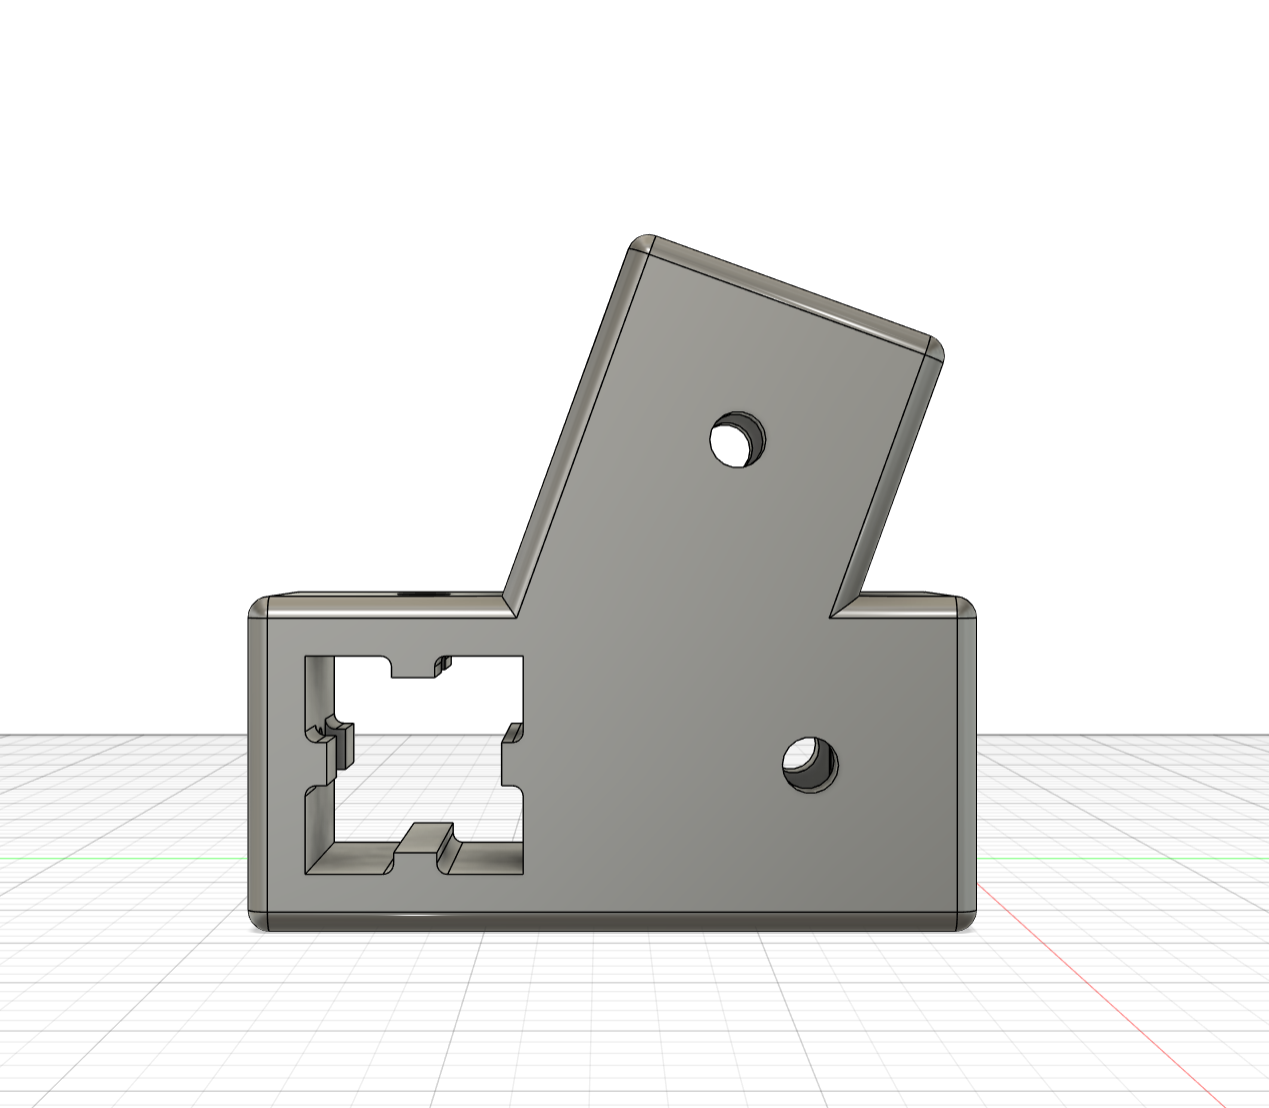
\includegraphics[width=0.6\textwidth]{Pieza_delantera_angulo_vistalateral.png}
    \caption{Vista lateral de la pieza de unión delantera, donde se aprecia la angulación de 70° prevista para el montante que sostiene el panel de acrílico. Fuente: Autora.}
    \label{fig:pieza_delantera_lateral}
\end{figure}

\begin{figure}[H]
    \centering
    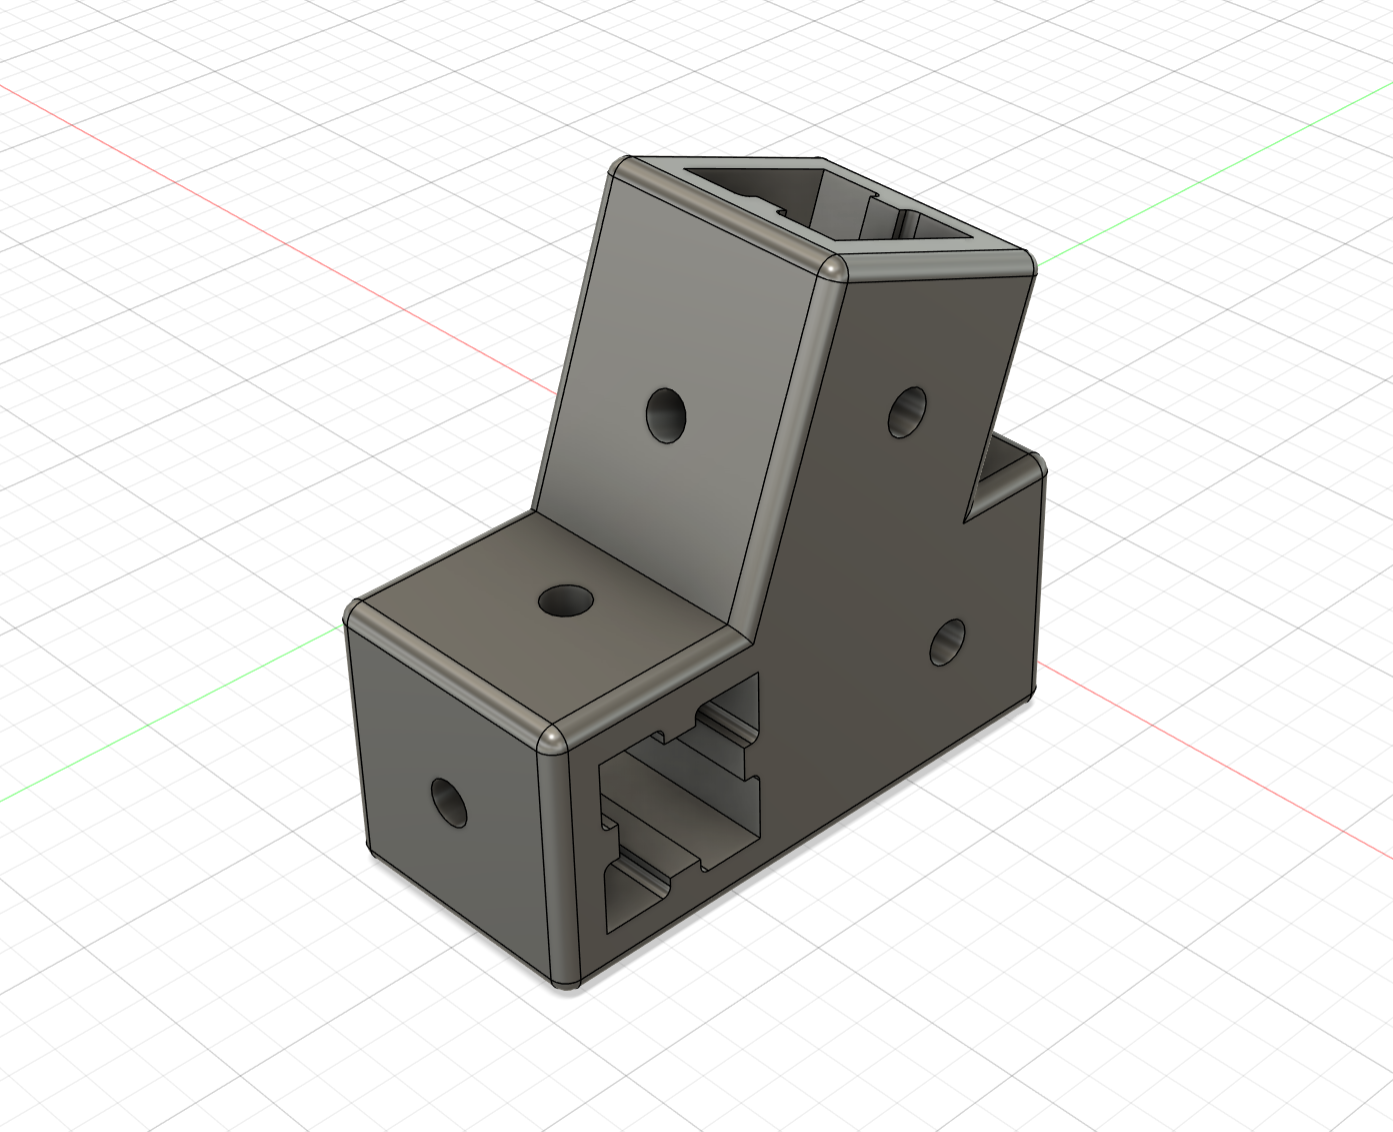
\includegraphics[width=0.75\textwidth]{Pieza_delantera_angulo_vistaperfil.png}
    \caption{Vista general de la pieza de unión delantera con angulación, diseñada para vincular tres perfiles en la esquina frontal de la estructura. Fuente: Autora.}
    \label{fig:pieza_delantera_perfil}
\end{figure}

Los codos traseros resuelven el encuentro de los perfiles en las esquinas posteriores de la base, donde no concurre ningún elemento inclinado. La Figura~\ref{fig:pieza_trasera_perfil} muestra la vista general del codo y la Figura~\ref{fig:pieza_trasera_superior} su vista superior, en la que se distingue la disposición de las perforaciones que reciben la tornillería.

\begin{figure}[H]
    \centering
    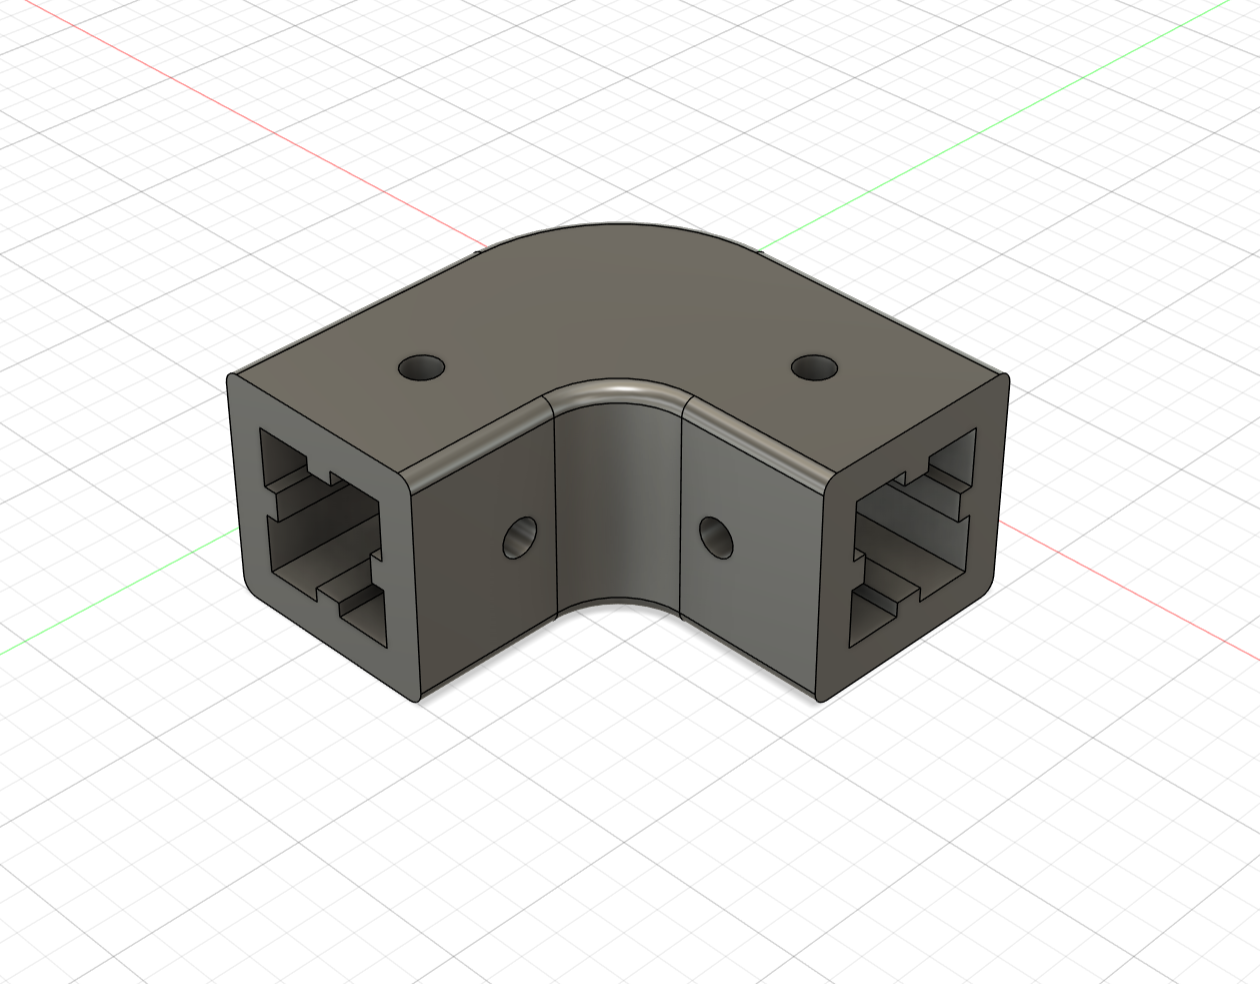
\includegraphics[width=0.75\textwidth]{Pieza_trasera_codo_vistaperfil.png}
    \caption{Vista general del codo de unión trasero de la estructura. Fuente: Autora.}
    \label{fig:pieza_trasera_perfil}
\end{figure}

\begin{figure}[H]
    \centering
    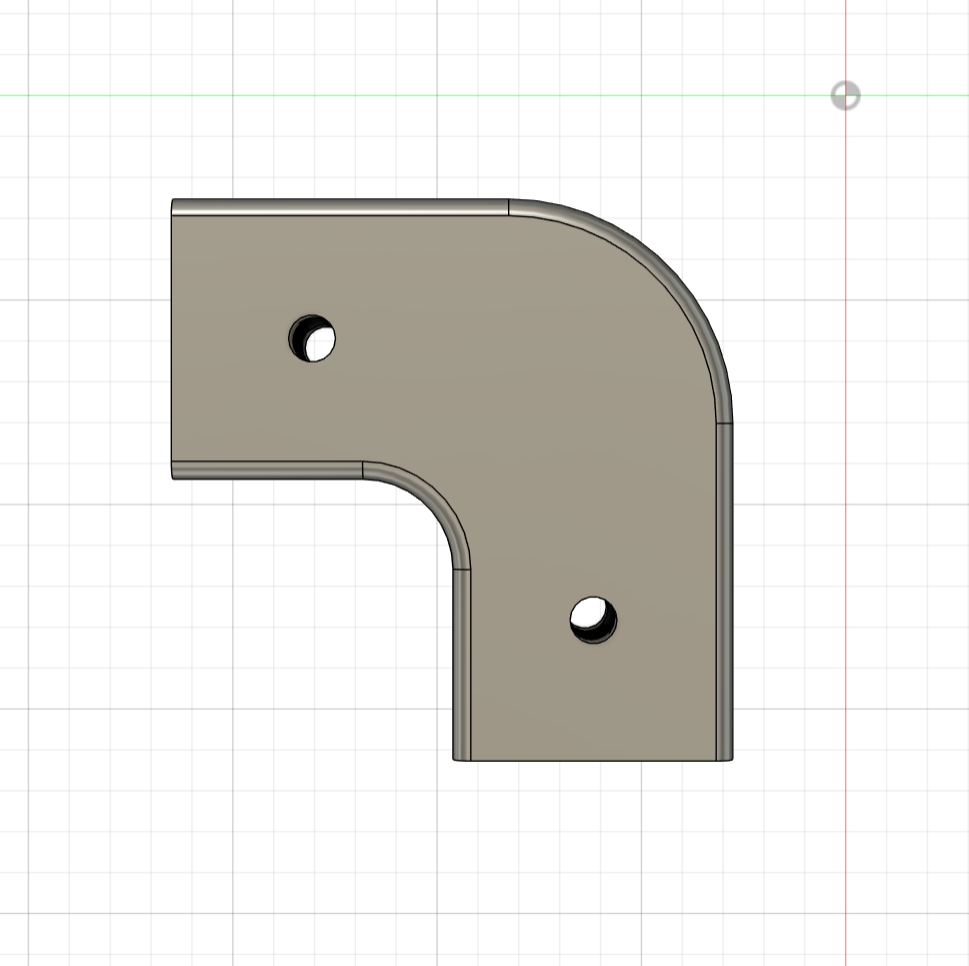
\includegraphics[width=0.6\textwidth]{Pieza_trasera_codo_vistasuperior.png}
    \caption{Vista superior del codo de unión trasero, donde se observa la disposición de las perforaciones de fijación. Fuente: Autora.}
    \label{fig:pieza_trasera_superior}
\end{figure}

Las cuatro piezas se fabricaron por impresión 3D en PLA. Este material se seleccionó por su disponibilidad, su bajo costo y su suficiencia mecánica para el esfuerzo al que las uniones quedan sometidas, que es fundamentalmente de compresión y no de tracción, dado que la carga del panel se transmite a la base a través de los propios perfiles.

% -------------------------------------------------
\subsubsection{Modelo de ensamble y producto esperado}
% -------------------------------------------------

Antes de proceder al montaje físico se verificó el ensamble completo en Fusion~360, integrando los perfiles ya seccionados según el plan de corte con las cuatro piezas de unión diseñadas. Esta verificación previa permitió confirmar la coherencia dimensional del conjunto y la correcta materialización del ángulo de 70° antes de realizar cortes irreversibles sobre la perfilería adquirida. La Figura~\ref{fig:estructura_esperada} presenta el producto esperado resultante de ese modelado.

\begin{figure}[H]
    \centering
    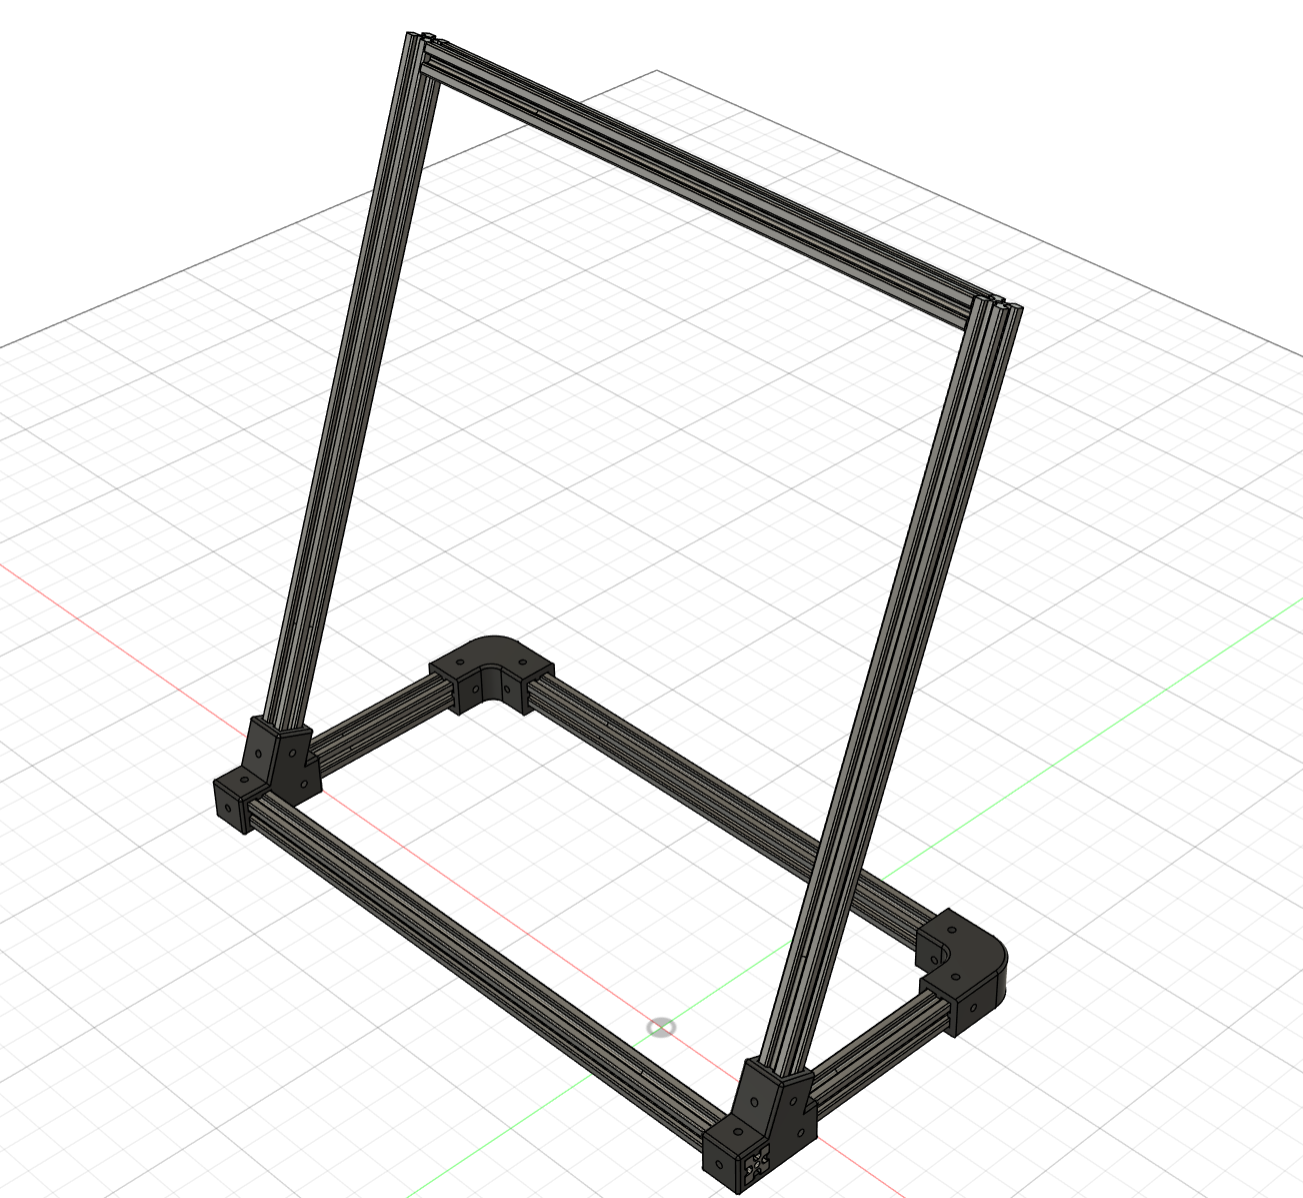
\includegraphics[width=0.8\textwidth]{Producto_estructura_esperado.png}
    \caption{Modelo de ensamble de la estructura de soporte, con las cuatro piezas de unión impresas en 3D vinculando los seis perfiles de aluminio ya seccionados. Fuente: Autora.}
    \label{fig:estructura_esperada}
\end{figure}

% -------------------------------------------------
\subsubsection{Montaje físico de la estructura}
% -------------------------------------------------

Verificado el modelo, se ejecutó el montaje físico de la plataforma. El ensamble requirió 14 tuercas T M5$\times$16, que son el elemento normalizado del sistema T-slot para fijar los elementos sin perforar el perfil. La tuerca se introduce en la ranura, gira un cuarto de vuelta hasta quedar retenida por los labios del perfil y recibe el tornillo desde el exterior, de modo que la unión puede reposicionarse a lo largo de todo el perfil sin practicar ningún agujero.

Entre la cabeza de cada tornillo y la pieza impresa se interpuso una arandela de acrílico negro fabricada en cortadora láser. Estas arandelas cumplen dos funciones: distribuyen la presión de la cabeza del tornillo sobre una superficie mayor de la pieza de PLA, lo que evita la marca por aplastamiento del material impreso y mejora el soporte de la unión, y unifican el acabado visual del conjunto. El diseño de corte se elaboró en el programa RDWorks y se presenta en la Figura~\ref{fig:arandela_laser}.

\begin{figure}[H]
    \centering
    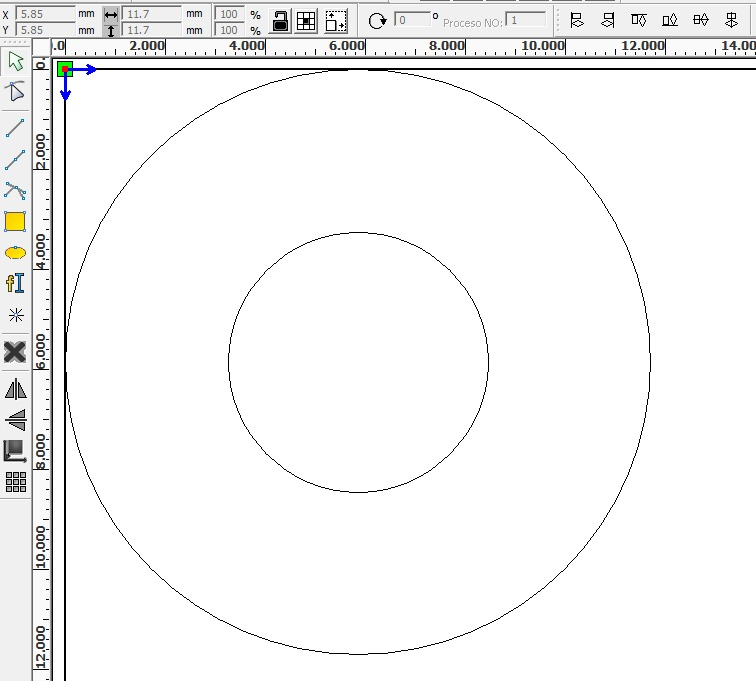
\includegraphics[width=0.7\textwidth]{Arandela_diseno_cortelaser.jpeg}
    \caption{Diseño de las arandelas de acrílico negro elaborado en RDWorks para su fabricación en cortadora láser. Fuente: Autora.}
    \label{fig:arandela_laser}
\end{figure}

El panel sobre el cual se empotra el sistema de control es una lámina de acrílico transparente de 5~mm de espesor. Este espesor se determinó a partir de la geometría del propio perfil, ya que la apertura de la ranura del perfil de 20$\times$20~mm es de 6~mm, de modo que una lámina de 5~mm encaja dentro de la ranura y queda retenida por los labios del perfil, con la holgura suficiente para deslizarla durante el montaje sin forzar el material. El panel se sostiene así por la propia ranura, sin requerir escuadras ni tornillería adicional para su fijación.

Con este montaje quedó concluida la estructura de soporte, que constituye el primer producto físico del proyecto y la base sobre la cual se instala el sistema de control.

% -------------------------------------------------
\subsubsection{Disposición de los componentes sobre el panel}
% -------------------------------------------------

Sobre esa estructura se monta el panel de control, que es el elemento con el que el estudiante interactúa, es decir, la lámina de acrílico descrita en la subsección anterior. La Figura~\ref{fig:plano_panel} muestra la disposición final de los componentes sobre el panel, que se organiza en tres rieles DIN separados por canaletas ranuradas (cuatro horizontales y dos verticales) por las que corre el cableado interno:

\begin{itemize}
    \item \textbf{Riel 1, control:} el Arduino Opta WiFi (A1) y, a su derecha, la expansión analógica A0602 (A2), unidos por el bus AUX.
    \item \textbf{Riel 2, alimentación e interfaces:} el DIN Simul8 (A3), por donde entra la energía del panel; la tarjeta optoacopladora PC817 (A4); y las borneras de distribución de 0~V (X0V) y de +24~V (X24V).
    \item \textbf{Riel 3, regleta del estudiante:} ocho grupos de borneras de paso (X1 a X8), rotulados en la canaleta superior según la función de cada grupo.
\end{itemize}

La disposición sigue el flujo lógico de la señal, de arriba hacia abajo, del controlador a la regleta, de modo que todo cable interno baja desde su módulo hacia el grupo de borneras que le corresponde. Toda la plataforma queda a la vista del estudiante sobre el panel, pero las conexiones de cada práctica se hacen en la regleta del riel 3, lo que evita cablear directamente sobre los bornes del hardware de control durante la experimentación y estandariza el punto de conexión con independencia de la práctica que se realice. Los dispositivos de campo (sensores, actuadores y elementos de instrumentación de bajo costo) quedan así desacoplados del núcleo de control y pueden variarse, sustituirse o ampliarse sin intervenir el montaje interno.

La Tabla~\ref{tab:equipos_panel} identifica cada equipo y grupo de borneras rotulado en la Figura~\ref{fig:plano_panel} y el riel en que se ubica.

\begin{figure}[H]
    \centering
    \figuraexterna{trim=39 31 34 33,clip,height=0.93\textheight,width=\linewidth,keepaspectratio}{Plano_Panel_Control.pdf}
    \caption{Disposición de los componentes sobre el panel de control, tal como quedó montado. Fuente: Autora.}
    \label{fig:plano_panel}
\end{figure}

\begin{table}[H]
\centering
\caption{Lista de equipos y borneras del panel de control. Fuente: Autora.}
\label{tab:equipos_panel}
\renewcommand{\arraystretch}{1.3}
\begin{tabularx}{\textwidth}{|p{1.8cm}|X|p{2.4cm}|}
\hline
\filacolor{TableGray}
\textbf{Ref.} & \textbf{Descripción} & \textbf{Ubicación} \\
\hline
A1 & Arduino Opta WiFi (micro-PLC) & Riel 1 \\
\hline
A2 & Módulo de expansión A0602 (AFX00007), conectado al A1 por el bus AUX & Riel 1 \\
\hline
A3 & DIN Simul8, placa de ocho interruptores con bloque de alimentación & Riel 2 \\
\hline
A4 & Tarjeta optoacopladora PC817 de cuatro canales & Riel 2 \\
\hline
X0V & Distribución de 0~V con cinco bornes verde/amarillo de doble nivel & Riel 2 \\
\hline
X24V & Distribución de +24~V con bornes rojos multinivel (unos ocho) & Riel 2 \\
\hline
X1--X8 & Regleta del estudiante, con ocho grupos rotulados en la canaleta 3 & Riel 3 \\
\hline
\end{tabularx}
\end{table}

% -------------------------------------------------
\subsection{Núcleo de control y módulo de expansión}
\label{subsec:hw_control}
% -------------------------------------------------

El núcleo de control lo constituye el Arduino Opta WiFi, cuyas especificaciones y terminales se detallan en la Sección~\ref{sec:opta} y en la Tabla~\ref{tab:modulos}. Aporta ocho entradas configurables como digitales o analógicas de 0 a 10~V y cuatro salidas de relé de contacto seco, y se programa desde el computador por su puerto USB-C~\cite{ref8}.

A su derecha, en el mismo riel, se monta el módulo de expansión analógica A0602 (AFX00007), que amplía la plataforma hacia señales de 0--10~V, 4--20~mA y RTD (PT100), dos salidas analógicas y cuatro salidas PWM~\cite{ref35}. Es el único módulo que se enlaza con el controlador por el bus AUX, que resuelve la comunicación entre ambos; la energía, en cambio, no viaja por ese bus, porque el A0602 requiere su propia alimentación de 12 a 24~V~DC~\cite{ref35}, que en la plataforma se toma de la distribución de 24~V del panel. Sus salidas PWM necesitan además una tensión externa de 8 a 24~V en el borne \texttt{VPWM}~\cite{ref35}, que también se toma de esa distribución.

El DIN Simul8, en cambio, no tiene puerto AUX; es una placa independiente que se cablea a tornillo. Cumple dos funciones en el panel: sus ocho interruptores sirven como entradas digitales simuladas para las primeras pruebas de programación, y su bloque de alimentación es el punto por el que la energía entra al panel (Sección~\ref{subsec:hw_alimentacion}).

El módulo DIN Celsius, incluido también en el kit, no se monta sobre el panel de control, sino que se reserva como sensor de prueba externo para las prácticas de temperatura, de modo que el estudiante lo conecte a la regleta únicamente cuando la práctica lo requiera. Contiene dos circuitos calentadores independientes de unos 120~mW cada uno y un sensor de temperatura TMP236 con salida de 0 a 10~V~\cite{ref37}. Esta decisión libera espacio útil en el riel y mantiene el panel limitado a los módulos de uso permanente.

El conjunto así integrado cubre el espectro de señales industriales más frecuente en aplicaciones de automatización educativa: entradas digitales a 24~V, entradas analógicas de tensión y de corriente, medida de temperatura por RTD, salidas de relé, salidas analógicas y salidas PWM.

% -------------------------------------------------
\subsection{Interfaz de acoplamiento con circuitos de baja tensión}
\label{subsec:hw_opto}
% -------------------------------------------------

La interfaz de acoplamiento es una tarjeta optoacopladora de cuatro canales basada en el PC817, montada en el riel 2. Admite señales de entrada entre 3,6 y 24~V y gobierna salidas entre 3,6 y 30~V~\cite{ref13}, y cada uno de sus canales aporta una tensión de aislamiento de 5\,000~V~rms con una CTR mínima del 50~\%~\cite{ref14}; cubre por tanto de forma directa, sin electrónica intermedia, el nivel del controlador en la entrada y, en la salida, cualquier tensión de alimentación dentro de ese rango.

Cada canal tiene, en el lado de entrada, el LED del PC817 en serie con un LED indicador y una resistencia limitadora de 3~k$\Omega$ integrados en la tarjeta, y en el lado de salida, una resistencia de \emph{pull-up} de 3~k$\Omega$ hacia el colector del fototransistor; ambos lados se verificaron en banco antes del montaje. Con 24~V en la entrada, y tomando del orden de 1,2~V para el LED del optoacoplador y 2~V para el LED indicador, la corriente de cada canal resulta
\begin{equation}
    I_{\mathrm{IN}} \approx \frac{24~\mathrm{V} - 1{,}2~\mathrm{V} - 2{,}0~\mathrm{V}}{3~\mathrm{k}\Omega} \approx 6{,}9~\mathrm{mA},
    \label{eq:pc817_corriente}
\end{equation}
suficiente para saturar el fototransistor con la CTR mínima indicada y despreciable frente a la capacidad de la fuente del panel. En el lado de salida, el borne \texttt{V} se alimenta con la fuente del circuito del estudiante y se lee en ese mismo punto. En reposo marca la tensión de esa fuente y cae hacia el nivel de \texttt{G} cuando el canal se activa. El estudiante elige esa tensión según las necesidades de su circuito, siempre dentro del rango admitido de 3,6 a 30~V. El caso de referencia en este documento es 5~V, por ser la alimentación habitual en los laboratorios de electrónica de la carrera, pero el mismo canal funciona igual con 9, 12 o 24~V.

La tarjeta trae un puente de configuración de tierra por canal. Los cuatro puentes se retiraron, de modo que cada canal queda con su referencia \texttt{G} aislada de las demás y del 0~V del panel; así la plataforma puede gobernar hasta cuatro circuitos del estudiante completamente independientes entre sí, incluso alimentados con tensiones distintas. Las salidas de la tarjeta se llevan al grupo OPTOCOUPLER OUTPUT de la regleta.

Su propósito es diversificar el alcance de la plataforma más allá del dominio industrial de 24~V~DC, integrando a un sistema gobernado por PLC los circuitos electrónicos que el estudiante construye en los demás laboratorios de la carrera. Con ello, la electrónica de baja tensión y el control industrial dejan de ser prácticas separadas y pueden combinarse en un diseño de mayor alcance que el que cualquiera de las dos permite por sí sola, mientras que el acoplamiento óptico mantiene ambos dominios eléctricamente separados y sin referencia de tierra común, según el principio expuesto en la Sección~\ref{subsec:optoacoplador}. El criterio de fondo es entregar al estudiante las herramientas que su propio diseño pueda requerir, de modo que la plataforma no imponga un límite a lo que sea capaz de proponer.

% -------------------------------------------------
\subsection{Sistema de alimentación y distribución a 24~V~DC}
\label{subsec:hw_alimentacion}
% -------------------------------------------------

La plataforma se alimenta con el adaptador de 24~V~DC y 1~A que trae el kit AKX00051~\cite{ref36}, conectado al tomacorriente. Su salida entra por el conector tipo \emph{jack} del DIN Simul8, cuyo bloque de alimentación la entrega en sus bornes \texttt{+24V} y \texttt{GND}. Desde ahí, la energía pasa a las borneras de distribución del riel 2 (X24V y X0V) y de ellas se derivan el Opta, la alimentación del A0602, el borne \texttt{VPWM} de las salidas PWM, los comunes de los relés y el grupo de 24~V de la regleta, que alimenta los dispositivos de campo. Un único punto de entrada de energía simplifica la puesta en marcha (el panel se energiza o se apaga desde un solo conector) y garantiza que todos los módulos compartan la misma referencia de 0~V, condición necesaria para que el controlador lea correctamente las señales de los demás módulos.

El lado de salida de la interfaz de acoplamiento no se alimenta desde esta distribución, pues cada canal recibe la fuente del circuito del estudiante, de modo que ambos dominios eléctricos no comparten fuente ni referencia.

El criterio de dimensionamiento es que la suma de las cargas conectadas simultáneamente no supere la capacidad del adaptador. La Tabla~\ref{tab:balance_potencia} reúne el consumo de cada carga en la configuración más exigente que se usó, la de la Práctica~2 (Sección~\ref{subsec:res_p2}), en la que funcionan a la vez los calentadores del DIN Celsius y el motor del ventilador. Para cada carga, la corriente se obtiene de su potencia como $I = P/V$ con $V = 24$~V.

\begin{table}[H]
\centering
\caption{Balance de consumo a 24~V~DC en la configuración más exigente (Práctica~2). Fuente: Autora.}
\label{tab:balance_potencia}
\renewcommand{\arraystretch}{1.3}
\begin{tabularx}{\textwidth}{|X|p{3.2cm}|p{2.6cm}|}
\hline
\filacolor{TableGray}
\textbf{Carga} & \textbf{Dato} & \textbf{Corriente [mA]} \\
\hline
Arduino Opta WiFi & 2,2~W (máximo)~\cite{ref34} & 92 \\
\hline
Expansión A0602 & 1,8~W~\cite{ref35} & 75 \\
\hline
DIN Celsius, dos calentadores & $2 \times 0{,}12$~W~\cite{ref37} & 10 \\
\hline
Tarjeta PC817, cuatro canales activos & $4 \times 6{,}9$~mA (Ec.~\ref{eq:pc817_corriente}) & 28 \\
\hline
Motor de corriente continua (ventilador) & 0,5~A (placa) & 500 \\
\hline
\filacolor{TableGray}
\textbf{Total} & & \textbf{705} \\
\hline
\end{tabularx}
\end{table}

El consumo total es de unos 705~mA, el 71~\% de la capacidad del adaptador, con un margen cercano a 0,3~A. De este balance se desprende la regla de uso de la plataforma: las cargas de campo que se agreguen en una práctica no deben superar en conjunto ese margen; una carga mayor, como un motor de más potencia o varias electroválvulas a la vez, debe alimentarse con una fuente externa y gobernarse desde la plataforma mediante los contactos de relé. Del lado del cableado, las borneras de paso de 2,5~mm$^2$ que forman la regleta admiten 20~A, muy por encima de la corriente máxima que puede entregar el adaptador, por lo que no constituyen una limitación.

% -------------------------------------------------
\subsection{Regleta de terminales e identificación del cableado}
\label{subsec:hw_terminales}
% -------------------------------------------------

Aunque toda la plataforma queda a la vista sobre el panel, la regleta del riel 3 es el punto donde el estudiante conecta los dispositivos de campo, por lo que su identificación es parte del diseño y no un acabado posterior. Esta regleta agrupa las señales por función, en ocho grupos rotulados de izquierda a derecha: salidas del EasyPort (X1), salidas del optoacoplador (X2), entradas digitales (X3), salidas de relé (X4), entradas analógicas (X5), salidas analógicas (X6), salidas PWM (X7) y 24~V (X8). Los grupos de relés y de entradas analógicas incluyen bornes de 0~V, para que el estudiante tome la referencia en el mismo grupo en que conecta la señal. Las borneras de distribución X24V y X0V, en cambio, quedan en el riel 2, en una zona físicamente separada de la regleta de señales.

El cableado interno sigue un código de colores por tipo de señal (Tabla~\ref{tab:codigo_colores}), complementado con marcadores numéricos en cada cable. El color identifica la familia de la señal y el número, el canal. Para la alimentación, el número reproduce el valor lógico de la tensión: 1 para +24~V y 0 para 0~V. Así, un cable verde marcado con 3 es la entrada digital 3, y un cable café marcado con 2, la salida de relé 2.

\begin{table}[H]
\centering
\caption{Código de colores y etiquetas del cableado interno del panel de control. Fuente: Autora.}
\label{tab:codigo_colores}
\renewcommand{\arraystretch}{1.3}
\begin{tabularx}{\textwidth}{|p{3cm}|X|p{3.4cm}|}
\hline
\filacolor{TableGray}
\textbf{Color} & \textbf{Señal} & \textbf{Etiqueta} \\
\hline
Rojo & Alimentación +24~V~DC & 1 \\
\hline
Negro & Referencia 0~V (GND) & 0 \\
\hline
Verde & Entradas digitales del Opta (I1--I8) & 1--8, n.º de entrada \\
\hline
Café & Salidas de relé del Opta (O1--O4) & 1--4, n.º de relé \\
\hline
Azul & Entradas analógicas del A0602 (I1--I6) & 1--6, n.º de entrada \\
\hline
Marrón-naranja & Salidas analógicas del A0602 (O1--O2) & 1--2, n.º de salida \\
\hline
Blanco & Salidas PWM del A0602 (P1--P4) & 1--4, n.º de salida \\
\hline
\end{tabularx}
\end{table}

La Figura~\ref{fig:diagrama_electrico} presenta el diagrama eléctrico completo del panel, dibujado sobre las fotografías de los módulos para que el estudiante reconozca cada borne en el equipo real. En él se observa el recorrido de cada cable desde su módulo hasta la regleta, con el color y la etiqueta del código anterior, y las dos barras de distribución de +24~V y 0~V de las que se alimentan todos los módulos.

% Página horizontal: afterpage la coloca tras la página en curso sin cortar el texto
% Margenes reducidos solo en esta pagina (se conserva el de encuadernacion) para agrandar el diagrama
\afterpage{%
\newgeometry{left=3cm,right=1.5cm,top=2cm,bottom=1.5cm}
\begin{landscape}
\begin{figure}[p]
    \centering
    \figuraexterna{trim=13 9 110 15,clip,width=\linewidth,height=0.91\textheight,keepaspectratio}{Diagrama_Electrico_Plataforma.pdf}
    \caption{Diagrama eléctrico del panel de control, con el código de colores y las etiquetas del cableado interno. Fuente: Autora.}
    \label{fig:diagrama_electrico}
\end{figure}
\end{landscape}
\restoregeometry}

% -------------------------------------------------
\subsection{Dispositivos de campo: sensor, pulsadores y luces}
\label{subsec:hw_campo}
% -------------------------------------------------

Los dispositivos de campo son los elementos que el estudiante conecta a la regleta para ejercitar las entradas y salidas del controlador: un sensor de proximidad como entrada representativa del entorno industrial, un juego de botones que aportan entradas de mando y un juego de luces indicadoras como cargas de salida. Complementan las tres decisiones de arquitectura de la Sección~\ref{sec:analisis_soluciones} y quedan por fuera del montaje de la plataforma, es decir, no se fijan al panel, sino que se conectan a él a través de la regleta. Su selección se documenta en las Secciones~\ref{subsec:alternativas_sensor} y~\ref{subsec:seleccion_sensor}; a continuación se describen los dispositivos seleccionados.

% -------------------------------------------------
\subsubsection{Sensor de proximidad}
\label{subsubsec:hw_sensor}
% -------------------------------------------------

El sensor de proximidad de la plataforma es el inductivo LJ12A3-4-Z/BY, que obtuvo el mayor puntaje ponderado (4{,}52) en la matriz de Pugh de la Tabla~\ref{tab:comparacion_sensor_proximidad} (Sección~\ref{subsec:seleccion_sensor}). Tiene 4~mm de alcance y se usa en su versión PNP normalmente abierta, con alimentación de 24~V~DC, por lo que se conecta directamente a cualquiera de las entradas I1--I8 del Opta, sin resistencia externa. Detecta objetos metálicos, el caso de detección más frecuente en la automatización industrial~\cite{ref23}, y opera sin ajuste previo. Junto con los botones y las luces indicadoras descritos en la sección siguiente, completa el juego de dispositivos de campo con que el estudiante construye prácticas de lógica de control con entradas y salidas industriales reales.

% -------------------------------------------------
\subsubsection{Dispositivos de indicación y mando}
\label{subsubsec:hw_indicacion_mando}
% -------------------------------------------------

Para que el estudiante pueda enviar órdenes al controlador y observar el resultado de su lógica con dispositivos físicos (y no solo con los interruptores y pilotos del módulo DIN Simul8, reservados como herramienta de simulación), la plataforma incorpora dos juegos de dispositivos de campo cableados a las borneras: un juego de botones pulsadores que aportan entradas de mando y un juego de luces indicadoras que actúan como cargas de salida.

\textbf{Juego de luces indicadoras.} Se seleccionó un juego de cinco luces piloto LED de 10~mm con cuerpo metálico, cinco colores distintos, alimentación de 12 a 24~V~DC y conductores ya soldados~\cite{ref25}. Cada luz se comporta como una carga de salida de bajo consumo que los contactos de relé del Opta gobiernan de forma directa (conmutando el positivo de 24~V hacia el terminal de la luz) o, si la práctica lo requiere, a través de la tarjeta optoacopladora, sin etapa de potencia adicional. Los cinco colores permiten que el estudiante asocie visualmente cada salida a un estado del proceso y que una misma práctica ejercite varias salidas simultáneas. La Figura~\ref{fig:luces_indicadoras} muestra el juego.

\begin{figure}[H]
    \centering
    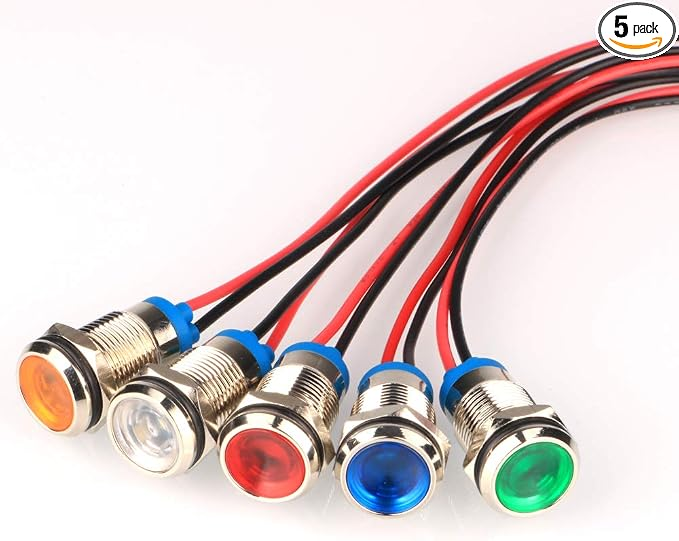
\includegraphics[width=0.55\textwidth]{Leds_24v}
    \caption{Juego de cinco luces piloto LED de 24~V~DC con cuerpo metálico~\cite{ref25}.}
    \label{fig:luces_indicadoras}
\end{figure}

\textbf{Juego de botones pulsadores.} Se seleccionó un juego de cinco botones pulsadores de 12~mm en acero inoxidable, de acción momentánea (cierran el contacto mientras se mantienen presionados y lo abren al soltarlos), con capacidad de 2~A y tensión de trabajo de hasta 250~V~AC, y conductores ya soldados~\cite{ref26}. Al ser un contacto seco, cada botón se conecta entre el positivo de 24~V y una entrada del Opta, de modo que al presionarlo la entrada recibe el nivel activo directamente, sin resistencias externas, tal como admiten las entradas del controlador~\cite{ref8}. La acción momentánea es la adecuada para ejercicios de marcha y paro, pulso de avance y detección de flanco, en los que el enclavamiento se resuelve por software; disponer de cinco unidades permite construir prácticas con varias entradas de mando. La Figura~\ref{fig:boton_pulsador} muestra el dispositivo y su modo de operación.

\begin{figure}[H]
    \centering
    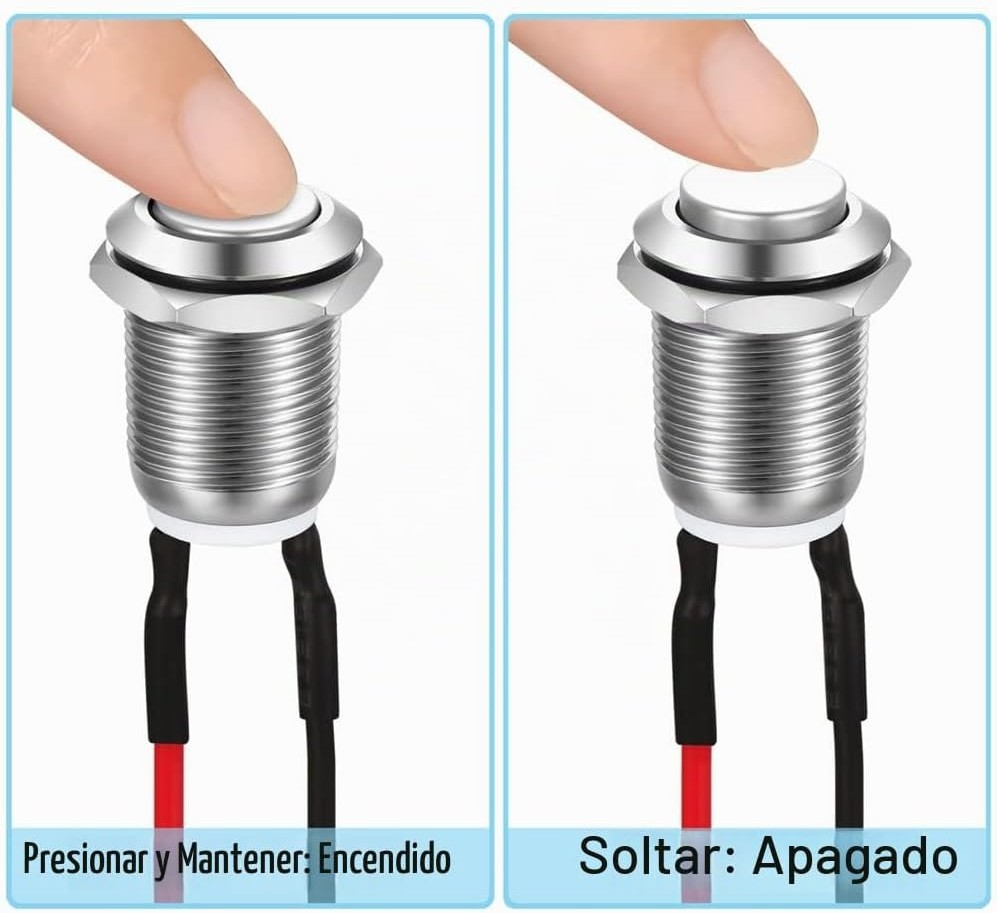
\includegraphics[width=0.55\textwidth]{Interruptor_boton}
    \caption{Botón pulsador metálico de 24~V de acción momentánea: contacto cerrado mientras se presiona, abierto al soltar~\cite{ref26}.}
    \label{fig:boton_pulsador}
\end{figure}

Ambos juegos comparten el dominio de 24~V~DC del resto de la plataforma, quedan por fuera de su montaje y llegan precableados, de modo que el estudiante los conecta a las borneras identificadas sin herramienta de soldadura. Los pulsadores y las luces indicadoras se emplearon en la Práctica~1 (Sección~\ref{subsec:res_p1}).

% -------------------------------------------------
\subsection{Normas y estándares aplicados}
\label{subsec:hw_normas}
% -------------------------------------------------

El diseño del hardware se apoyó en las siguientes normas internacionales:

\begin{itemize}
    \item \textbf{IEC 61131-3}~\cite{ref38}: define los lenguajes de programación de los controladores programables. Es el criterio que llevó a seleccionar el Arduino Opta (Sección~\ref{subsec:seleccion_unidad}) y el marco de todos los programas de la plataforma (Sección~\ref{sec:iec}).
    \item \textbf{IEC 60715}~\cite{ref39}: normaliza el riel de montaje de 35~mm sobre el que se instalan el Opta, la expansión A0602, el DIN Simul8 y las borneras de paso. Al usar este riel, cualquier módulo o bornera de formato industrial puede agregarse al panel sin modificarlo.
    \item \textbf{IEC 61140}~\cite{ref41}: clasifica como muy baja tensión las tensiones continuas que no superan 120~V. Toda la plataforma opera a 24~V~DC o menos, y la única conexión a la red eléctrica es el adaptador externo del kit, de modo que el estudiante nunca manipula conductores con tensión de red.
    \item \textbf{IEC 60204-1}~\cite{ref40}: recomienda identificar los conductores por colores según la función del circuito. La plataforma adopta ese principio de identificación por colores, pero con un código propio por tipo de señal (Tabla~\ref{tab:codigo_colores}), porque su finalidad es didáctica, ya que se busca que el estudiante distinga a simple vista una entrada digital de una analógica o de una salida PWM.
\end{itemize}

% -------------------------------------------------
\section{Descripción del software}
\label{sec:software}
% -------------------------------------------------

El software de la plataforma se divide en dos partes que se ejecutan en equipos distintos: el programa que corre en el Arduino Opta, que lee las entradas, ejecuta la lógica de control y escribe las salidas; y las aplicaciones del computador, con las que se escribe y depura ese programa y se simula la planta virtual. Ambas se describen por separado; las dos prácticas con que se verificó el funcionamiento de la plataforma se presentan como resultados en el Capítulo~\ref{chp:resultados}.

% -------------------------------------------------
\subsection{Software del controlador}
\label{subsec:sw_controlador}
% -------------------------------------------------

El Opta se programa desde el entorno Arduino PLC IDE, que admite los tres lenguajes normados por IEC~61131-3 contemplados en el alcance de este proyecto (Ladder Diagram, Function Block Diagram y Structured Text), cuyos fundamentos se exponen en la Sección~\ref{sec:iec}. Todo proyecto de la plataforma se organiza en cuatro elementos:

\begin{itemize}
    \item \textbf{Configuración del hardware:} el entorno detecta la expansión A0602 conectada por el bus AUX y la incorpora al proyecto. La expansión requiere el \emph{firmware} 0.1.8 o superior; con la versión 0.1.4 que traía el módulo, la salida PWM no respondía, por lo que se actualizó a la 0.1.14.
    \item \textbf{Mapeo de entradas y salidas:} a cada canal físico (entradas y relés del Opta, canales programables y salidas PWM de la expansión) se le asigna una variable global con nombre, que es la que usan los programas. El tipo de cada canal (digital, entrada de tensión, salida de tensión) se fija en este mismo paso.
    \item \textbf{Variables locales:} los valores intermedios y las constantes de cada programa (temporizadores, ganancias, escalas) se declaran dentro del programa que los usa.
    \item \textbf{Tareas y programas:} cada programa se asigna a una tarea, que lo ejecuta de forma cíclica. En cada ciclo de escaneo el controlador lee las entradas, ejecuta el programa y actualiza las salidas. Las prácticas con la expansión analógica se ejecutan en una tarea periódica de 50~ms.
\end{itemize}

El principio de funcionamiento de los algoritmos se ilustra con los dos programas desarrollados para las prácticas de verificación. El primero (Figura~\ref{fig:flujo_p1}) es una máquina de estados secuencial, en la que un pulsador de arranque con autoenclave inicia la secuencia, tres temporizadores a la conexión encienden una tras otra las cuatro salidas a intervalos de 5~s, y un pulsador de parada, que actúa como permiso de marcha, corta la secuencia en cualquier estado y la devuelve al reposo.

\begin{figure}[H]
    \centering
    \linespread{1}\selectfont
    \begin{tikzpicture}[
        font=\footnotesize, node distance=0.45cm,
        >={Stealth[length=2mm]},
        proceso/.style={draw=DeepBlue, fill=SoftBlue, line width=0.8pt, align=center,
                        text width=5.2cm, minimum height=0.75cm},
        decision/.style={draw=DeepBlue, fill=white, line width=0.8pt, diamond, aspect=2.6,
                         align=center, inner sep=1pt, text width=2.6cm},
        extremo/.style={draw=DeepBlue, fill=TableGray, line width=0.8pt, rounded corners=8pt,
                        align=center, minimum height=0.7cm, text width=2.6cm},
        flecha/.style={->, draw=DeepBlue, line width=0.8pt}
    ]
        \node[extremo] (ini) {Inicio};
        \node[proceso, below=of ini] (rep) {Reposo: \texttt{Led1} a \texttt{Led4} apagados};
        \node[decision, below=of rep] (p1) {¿Pulsador~1 presionado?};
        \node[proceso, below=of p1] (s1) {Autoenclave activo; enciende \texttt{Led1} e inicia \texttt{Timer1} (5~s)};
        \node[proceso, below=of s1] (s2) {Al cumplirse \texttt{Timer1}: enciende \texttt{Led2} e inicia el segundo temporizador};
        \node[proceso, below=of s2] (s3) {A los 10~s: enciende \texttt{Led3} e inicia el tercer temporizador};
        \node[proceso, below=of s3] (s4) {A los 15~s: enciende \texttt{Led4}};
        \node[decision, below=of s4] (p2) {¿Pulsador~2 presionado?};
        \draw[flecha] (ini) -- (rep);
        \draw[flecha] (rep) -- (p1);
        \draw[flecha] (p1) -- node[right] {Sí} (s1);
        \draw[flecha] (p1.east) -- node[above] {No} ++(0.8,0) |- (rep.east);
        \draw[flecha] (s1) -- (s2);
        \draw[flecha] (s2) -- (s3);
        \draw[flecha] (s3) -- (s4);
        \draw[flecha] (s4) -- (p2);
        \draw[flecha] (p2.east) -- node[above] {No} ++(0.8,0) |- (s4.east);
        \draw[flecha] (p2.west) -- node[above] {Sí} ++(-1.6,0) |- (rep.west);
        \node[font=\scriptsize, text width=2.4cm, align=left, text=DeepBlue] at ([xshift=-2.5cm]s2.west)
            {El pulsador~2 corta el autoenclave en cualquier estado y apaga todas las salidas.};
    \end{tikzpicture}
    \caption{Diagrama de flujo del programa de la Práctica~1, secuencia de cinco estados. Fuente: Autora.}
    \label{fig:flujo_p1}
\end{figure}

El segundo programa (Figura~\ref{fig:flujo_p2}) es un lazo de control proporcional que se ejecuta completo en cada ciclo de la tarea de 50~ms. Primero actualiza el estado de los calentadores según los pulsadores; luego convierte la lectura del sensor en grados Celsius, calcula el error respecto a la temperatura deseada y obtiene la salida del controlador, limitada entre 0 y 100~\%; por último, escala esa salida para dos actuadores: el ancho de pulso de la salida PWM que mueve el motor del ventilador y el valor del convertidor digital-analógico que entrega la misma orden como tensión de 0 a 10~V.

Las relaciones que implementa el programa se obtienen de los datos del sensor y de mediciones en el banco. El sensor del DIN Celsius entrega 400~mV a 0~$^\circ$C y 19,5~mV por $^\circ$C, amplificados por 4,9 hasta un rango de 0 a 10~V~\cite{ref37}, y el convertidor de 16~bits de la expansión representa 10~V con 65\,535 cuentas; despejando la temperatura,
\begin{equation}
    T = 0{,}0015969 \cdot N_{\mathrm{ADC}} - 20{,}51 \quad [^\circ\mathrm{C}],
    \label{eq:temp}
\end{equation}
donde $N_{\mathrm{ADC}}$ es la lectura del convertidor. La salida del controlador, con ganancia proporcional $K_P = 5$ y temperatura deseada $T_{\mathrm{ref}} = 28~^\circ$C, es
\begin{equation}
    u = \min\!\left(\max\!\left(K_P\,(T - T_{\mathrm{ref}}),\,0\right),\,100\right) \quad [\%].
    \label{eq:control}
\end{equation}
Con un periodo PWM de 1000~$\mu$s, el ancho de pulso es $t_{\mathrm{on}} = 10 \cdot u$~[$\mu$s]; por ejemplo, con $u = 50~\%$ el pulso dura 500~$\mu$s. Para la salida analógica, la tensión medida en el borne de salida resultó proporcional al valor escrito, con 1,475~mV por cuenta; para que $u = 100~\%$ corresponda a 10~V se requieren unas 6780 cuentas, es decir, 67,8 cuentas por cada punto porcentual.

\begin{figure}[H]
    \centering
    \linespread{1}\selectfont
    \begin{tikzpicture}[
        font=\footnotesize, node distance=0.45cm,
        >={Stealth[length=2mm]},
        proceso/.style={draw=DeepBlue, fill=SoftBlue, line width=0.8pt, align=center,
                        text width=6.4cm, minimum height=0.75cm},
        extremo/.style={draw=DeepBlue, fill=TableGray, line width=0.8pt, rounded corners=8pt,
                        align=center, minimum height=0.7cm, text width=4.4cm},
        flecha/.style={->, draw=DeepBlue, line width=0.8pt}
    ]
        \node[extremo] (ini) {Inicio de ciclo (tarea de 50~ms)};
        \node[proceso, below=of ini] (a) {Pulsadores 1 y 2: alternan el estado de cada calentador al detectar el flanco; pulsador 3: apaga ambos};
        \node[proceso, below=of a] (b) {Relés \texttt{O1} y \texttt{O2} $\leftarrow$ estado de cada calentador};
        \node[proceso, below=of b] (c) {Lectura del sensor y conversión a $^\circ$C (Ec.~\ref{eq:temp})};
        \node[proceso, below=of c] (d) {Error: $e = T - T_{\mathrm{ref}}$};
        \node[proceso, below=of d] (e) {Salida del controlador: $u = K_P\,e$, limitada a 0--100~\% (Ec.~\ref{eq:control})};
        \node[proceso, below=of e] (f) {Salida PWM \texttt{P1}: ancho de pulso $= 10 \cdot u$~[$\mu$s] (motor del ventilador)};
        \node[proceso, below=of f] (g) {Salida analógica \texttt{O1}: $67{,}8 \cdot u$ cuentas (0--10~V hacia el EasyPort)};
        \node[extremo, below=of g] (fin) {Fin de ciclo};
        \foreach \x/\y in {ini/a, a/b, b/c, c/d, d/e, e/f, f/g, g/fin} \draw[flecha] (\x) -- (\y);
        \draw[flecha] (fin.east) -- ++(1.4,0) |- (ini.east);
    \end{tikzpicture}
    \caption{Diagrama de flujo del programa de la Práctica~2, control proporcional de temperatura. Fuente: Autora.}
    \label{fig:flujo_p2}
\end{figure}

% -------------------------------------------------
\subsection{Software del computador}
\label{subsec:sw_computador}
% -------------------------------------------------

En el computador se usan tres aplicaciones, todas sobre Windows:

\begin{itemize}
    \item \textbf{Arduino PLC IDE:} entorno de acceso gratuito en el que se configura el hardware, se escriben y compilan los programas y se descargan al Opta por el puerto USB-C. Con el programa en ejecución, su tabla de observación muestra en línea el valor de cada variable, lo que permite depurar la lógica sin instrumentos adicionales.
    \item \textbf{FluidSIM:} simulador de Festo en el que el estudiante dibuja la planta (cilindros, válvulas, relés y otros elementos de campo) y la pone en movimiento~\cite{ref28}. Mediante sus bloques de entrada y salida para el EasyPort, la planta virtual intercambia señales reales con el Opta, de modo que las salidas del controlador accionan los elementos simulados, y los elementos simulados entregan señales a las entradas del controlador (Sección~\ref{sec:fluidsim_easyport}).
    \item \textbf{Festo EasyPort Web Bridge:} aplicación del fabricante que muestra el estado de los canales del EasyPort. En la plataforma se utilizó para leer la tensión que la salida analógica del A0602 entrega a una entrada analógica del EasyPort.
\end{itemize}

El EasyPort se conecta al computador por USB y al panel por su cable SysLink, cuyos hilos llegan al grupo X1 de la regleta~\cite{ref27}. De este modo, el computador participa en la plataforma de dos maneras: como herramienta de programación del controlador y como planta virtual que el controlador gobierna.

% -------------------------------------------------
\section{Análisis costo-beneficio frente a PLC industriales convencionales}
\label{sec:costo_beneficio}
% -------------------------------------------------

Esta sección compara la plataforma con los sistemas PLC industriales convencionales en dos aspectos: el costo del hardware y del software necesarios para equipar un puesto de trabajo, y las características técnicas que respaldan que la comparación es entre sistemas funcionalmente equivalentes. Se tomó como referencia el PLC Siemens SIMATIC S7-1500, que es la plataforma sobre la que se construye el sistema Festo EduTrainer Universal que la Escuela utiliza actualmente (Sección~\ref{subsec:seleccion_unidad}).

\subsection{Comparación de costos}

Para el sistema convencional se armó la configuración mínima que cubre las entradas y salidas de la plataforma: la CPU 1513-1~PN ya considerada en la selección de la unidad de control, su fuente de sistema, el perfil de montaje, un módulo de 16 entradas digitales a 24~V y un módulo de 16 salidas digitales a 24~V, más la licencia del entorno de programación STEP~7 Professional. Para la plataforma se consideró el hardware de control del presupuesto: el kit AKX00051 y el módulo analógico AFX00007, con un entorno de programación gratuito. Los precios en euros son los publicados por los proveedores consultados, sin IVA, y se convirtieron a colones con el tipo de cambio implícito en el presupuesto (₡518,49 por euro) para que ambas columnas sean comparables con la Tabla~\ref{tab:presupuesto}. El EduTrainer se valoró con la cotización formal de ICE Electronics~\cite{ref47}, que está en dólares; se tomó su precio sin IVA y se convirtió con el tipo de cambio de ₡510 por dólar empleado en el presupuesto. De esa cotización se consideraron solo el equipo base EduTrainer y sus cables de conexión.

\begin{table}[H]
\centering
\caption{Comparación de costos de hardware y licencias de software entre la plataforma propuesta y un sistema PLC industrial convencional. Fuente: Autora.}
\label{tab:costo_beneficio}
\small\linespread{1}\selectfont
\renewcommand{\arraystretch}{1.5}
% Ancho total = columnas (13,8 cm) + 8 \tabcolsep + 5 lineas verticales
\newcommand{\lineagris}{\reglasuperior{\dimexpr13.8cm+8\tabcolsep+5\arrayrulewidth\relax}}
\begin{tabular}{|>{\raggedright\arraybackslash}p{7.3cm}|>{\centering\arraybackslash}p{1.9cm}|>{\raggedleft\arraybackslash}p{2.2cm}|>{\raggedleft\arraybackslash}p{2.4cm}|}
\hline
\filacolor{TableGray}
\textbf{Elemento} & \textbf{Ref.} & \textbf{Precio (EUR)} & \textbf{Total (₡)} \\
\hline
\filacolor{TableGrayDark}
\multicolumn{4}{|l|}{\lineagris\textit{Plataforma propuesta (Arduino Opta)}} \\
\hline
Kit Arduino PLC Starter Kit AKX00051 (Opta WiFi, DIN Simul8 y DIN Celsius) & Tabla~\ref{tab:presupuesto} & 431{,}00 & 223.470 \\
\hline
Módulo analógico de expansión AFX00007 & Tabla~\ref{tab:presupuesto} & 237{,}00 & 122.882 \\
\hline
Software Arduino PLC IDE & \cite{ref1} & Gratuito & 0 \\
\hline
\filacolor{TableGray}
\lineagris\textbf{Subtotal hardware de control} & & \textbf{668{,}00} & \textbf{346.352} \\
\hline
Tarjeta optoacopladora de 4 canales basada en el PC817 & \cite{ref13} & USD~5{,}95 & 3.034{,}50 \\
\hline
Estructura de soporte (perfilería de aluminio T-slot, escuadras, tuercas y tornillos) & Tabla~\ref{tab:presupuesto} & -- & 30.358{,}77 \\
\hline
Materiales eléctricos y de cableado (rieles DIN, ductos, borneras, cable y etiquetas) & Tabla~\ref{tab:presupuesto} & -- & 99.035{,}15 \\
\hline
\filacolor{TableGray}
\lineagris\textbf{Total plataforma (presupuesto)} & & & \textbf{478.780{,}42} \\
\hline
\filacolor{TableGrayDark}
\multicolumn{4}{|l|}{\lineagris\textit{Sistema convencional (Siemens SIMATIC S7-1500)}} \\
\hline
CPU 1513-1~PN (6ES7513-1AL02-0AB0) & \cite{ref17} & 1.746{,}51 & 905.548 \\
\hline
Fuente de sistema PS 25W 24~V~DC (6ES7505-0KA00-0AB0) & \cite{ref44} & 232{,}24 & 120.414 \\
\hline
Perfil de montaje de 245~mm (6ES7590-1AC40-0AA0) & \cite{ref45} & 31{,}98 & 16.581 \\
\hline
Módulo de 16 entradas digitales DI 16x24VDC HF (6ES7521-1BH00-0AB0) & \cite{ref42} & 203{,}09 & 105.300 \\
\hline
Módulo de 16 salidas digitales DQ 16x24VDC/0,5A (6ES7522-1BH01-0AB0) & \cite{ref43} & 215{,}76 & 111.869 \\
\hline
\filacolor{TableGray}
\lineagris\textbf{Subtotal hardware convencional} & & \textbf{2.429{,}58} & \textbf{1.259.712} \\
\hline
Licencia STEP~7 Professional V19, flotante (6ES7822-1AA23-0YA5) & \cite{ref46} & 3.896{,}20 & 2.020.141 \\
\hline
\filacolor{TableGray}
\lineagris\textbf{Total sistema convencional} & & \textbf{6.325{,}78} & \textbf{3.279.853} \\
\hline
\filacolor{TableGrayDark}
\multicolumn{4}{|l|}{\lineagris\textit{Sistema didáctico (Festo EduTrainer Universal)}} \\
\hline
EduTrainer Universal S7-1512C-1PN (8065595) con sus cables: datos SysLink (34031), analógicos paralelo y cruzado (529141 y 533039) y de potencia (549861) & \cite{ref47} & USD~7.562{,}17 & 3.856.707 \\
\hline
\end{tabular}
\end{table}

El hardware de control convencional cuesta unas 3,6 veces el de la plataforma, y con la licencia del entorno de programación el sistema completo llega a unas 9,5 veces; es decir, con lo que cuesta un solo puesto convencional se equiparían nueve puestos con la plataforma propuesta. El sistema didáctico que la Escuela utiliza actualmente amplía esa diferencia, ya que el equipo base del EduTrainer con sus cables cuesta ₡3.856.707, unas 11 veces el hardware de la plataforma (₡346.352), de modo que su precio equivale al de once puestos de la plataforma; además, al igual que el S7-1500, requiere la licencia de pago de TIA Portal (Tabla~\ref{tab:equivalencia_tecnica}). Esta cifra confirma la calificación de costo que el EduTrainer recibió en la selección de la unidad de control, equivalente a la de un PLC industrial completo (Sección~\ref{subsec:seleccion_unidad}).

Las tres relaciones son conservadoras respecto de lo que ofrece cada sistema. La configuración de Siemens no incluye módulos analógicos, ni los conectores frontales, ni la fuente de 24~V~DC que alimenta la propia fuente de sistema, y del EduTrainer solo se tomaron el equipo base y sus cables de conexión; en cambio, el hardware de la plataforma ya incluye entradas y salidas analógicas, salidas PWM, el módulo de interruptores DIN Simul8 y el sensor DIN Celsius.

\subsection{Equivalencia de características técnicas}

La Tabla~\ref{tab:equivalencia_tecnica} contrasta las características que importan para el uso didáctico. La plataforma cubre lo que exige un laboratorio de programación de PLC (lenguajes normados, señales industriales a 24~V, comunicación industrial y ampliación modular), y las diferencias recaen en la robustez de gama alta y en el ecosistema de licenciamiento de Siemens, que es lo que encarece el sistema convencional sin añadir valor formativo para el nivel del curso.

\begin{table}[H]
\centering
\caption{Equivalencia de características técnicas entre la plataforma propuesta y los sistemas convencionales. Fuente: Autora.}
\label{tab:equivalencia_tecnica}
\footnotesize
\renewcommand{\arraystretch}{1.3}
\renewcommand\tabularxcolumn[1]{m{#1}}
\begin{tabularx}{\textwidth}{|>{\raggedright\arraybackslash}m{2.8cm}|>{\raggedright\arraybackslash}X|>{\raggedright\arraybackslash}X|>{\raggedright\arraybackslash}X|}
\hline
\filacolor{TableGray}
\textbf{Característica} & \textbf{Plataforma (Opta WiFi y AFX00007)} & \textbf{Siemens S7-1500 (configuración de la Tabla~\ref{tab:costo_beneficio})} & \textbf{Festo EduTrainer Universal} \\
\hline
Lenguajes IEC 61131-3 & LD, FBD y ST~\cite{ref1,ref8} & LD, FBD y ST (SCL), entre otros & Los de TIA Portal \\
\hline
Entradas y salidas digitales & 8 entradas de 0 a 24~V~DC y 4 salidas de relé~\cite{ref8} & 16 entradas y 16 salidas a 24~V~DC (módulos de la Tabla~\ref{tab:costo_beneficio}) & Interruptores y pilotos con bornes de seguridad de 4~mm~\cite{ref18} \\
\hline
Señales analógicas y PWM & 6 entradas (0--10~V, 4--20~mA, RTD), 2 salidas y 4 salidas PWM~\cite{ref35} & Requiere módulos adicionales no incluidos & Según la configuración \\
\hline
Conectividad & Ethernet, WiFi, USB-C y RS-485 con Modbus~\cite{ref8} & PROFINET & PROFINET \\
\hline
Entorno de programación & Arduino PLC IDE, gratuito & TIA Portal, con licencia de pago & TIA Portal, con licencia de pago \\
\hline
Formato de montaje & Riel DIN, panel reconfigurable & Riel DIN, perfil de montaje & Banco cerrado, un puesto por unidad~\cite{ref18} \\
\hline
\end{tabularx}
\end{table}

En consecuencia, para el objetivo de enseñar programación de PLC con lenguajes normados y señales industriales, la plataforma ofrece una funcionalidad equivalente a una fracción del costo, y su entorno gratuito permite que el Campus replique, mantenga y amplíe el sistema sin pagar licencias, lo que responde de forma directa a la carencia de infraestructura planteada en el problema.


% =================================================================
\chapter{Resultados}
\label{chp:resultados}
% =================================================================

Este capítulo presenta los resultados del proyecto y los analiza conforme a los objetivos específicos planteados en el Capítulo~\ref{chp:metaobj}. Estos resultados abarcan el panel de control construido, la verificación de las señales industriales mediante las dos prácticas de laboratorio, la guía elaborada para los estudiantes y la comparación de costos y características con los PLC industriales convencionales. La Sección~\ref{sec:resultados} resume, para cada práctica, su objetivo, los materiales y equipos empleados y lo que se comprobó; el procedimiento paso a paso se encuentra en la guía de laboratorio, incluida completa en el Apéndice~\ref{chp:guia}. La Sección~\ref{sec:analisis} evalúa el cumplimiento de cada objetivo, con el panel, las señales verificadas y el análisis costo-beneficio, y cierra con los alcances y limitaciones de la solución implementada.

% -------------------------------------------------
\section{Resultados de las prácticas}
\label{sec:resultados}
% -------------------------------------------------

Las pruebas se realizaron con la plataforma completa en el banco de trabajo, con todas las conexiones hechas sobre la regleta del panel. El comportamiento de los programas se observó en la tabla de observación del Arduino PLC IDE, que muestra en línea el valor de cada variable mientras el controlador ejecuta la lógica; las tensiones de la salida analógica se midieron con un multímetro en el borne de salida, y la lectura del lado del computador se obtuvo con el Festo EasyPort Web Bridge (Sección~\ref{subsec:sw_computador}).

% -------------------------------------------------
\subsection{Práctica 1: secuencia de cinco estados}
\label{subsec:res_p1}
% -------------------------------------------------

\textbf{Objetivo.} Automatizar un proceso secuencial como los de una línea de producción, en este caso una estación que activa cuatro actuadores uno tras otro, a intervalos fijos, gobernada con un pulsador de arranque y uno de parada. El programa se escribe en Ladder Diagram y la parte neumática de la estación se simula en FluidSIM.

\textbf{Materiales.} Plataforma didáctica con el Arduino Opta WiFi, dos pulsadores sin enclavamiento de 24~V, cuatro luces indicadoras LED de 24~V, EasyPort USB con su cable SysLink, y computador con PLC IDE y FluidSIM.

\textbf{Resultados.} El programa de la Figura~\ref{fig:flujo_p1} se descargó en el Opta y se enlazó con la planta de FluidSIM a través del EasyPort. Los pulsadores, conectados a las entradas digitales de la regleta, arrancan y detienen la secuencia; los relés del Opta accionan los cilindros simulados en FluidSIM y las salidas del EasyPort encienden las luces indicadoras, de modo que cada estado se observa a la vez en la pantalla y en el equipo físico. La práctica valida las entradas digitales, las salidas de relé y el enlace entre el controlador real y la planta virtual. La Figura~\ref{fig:diagrama_p1} muestra las conexiones usadas.

\begin{figure}[H]
    \centering
    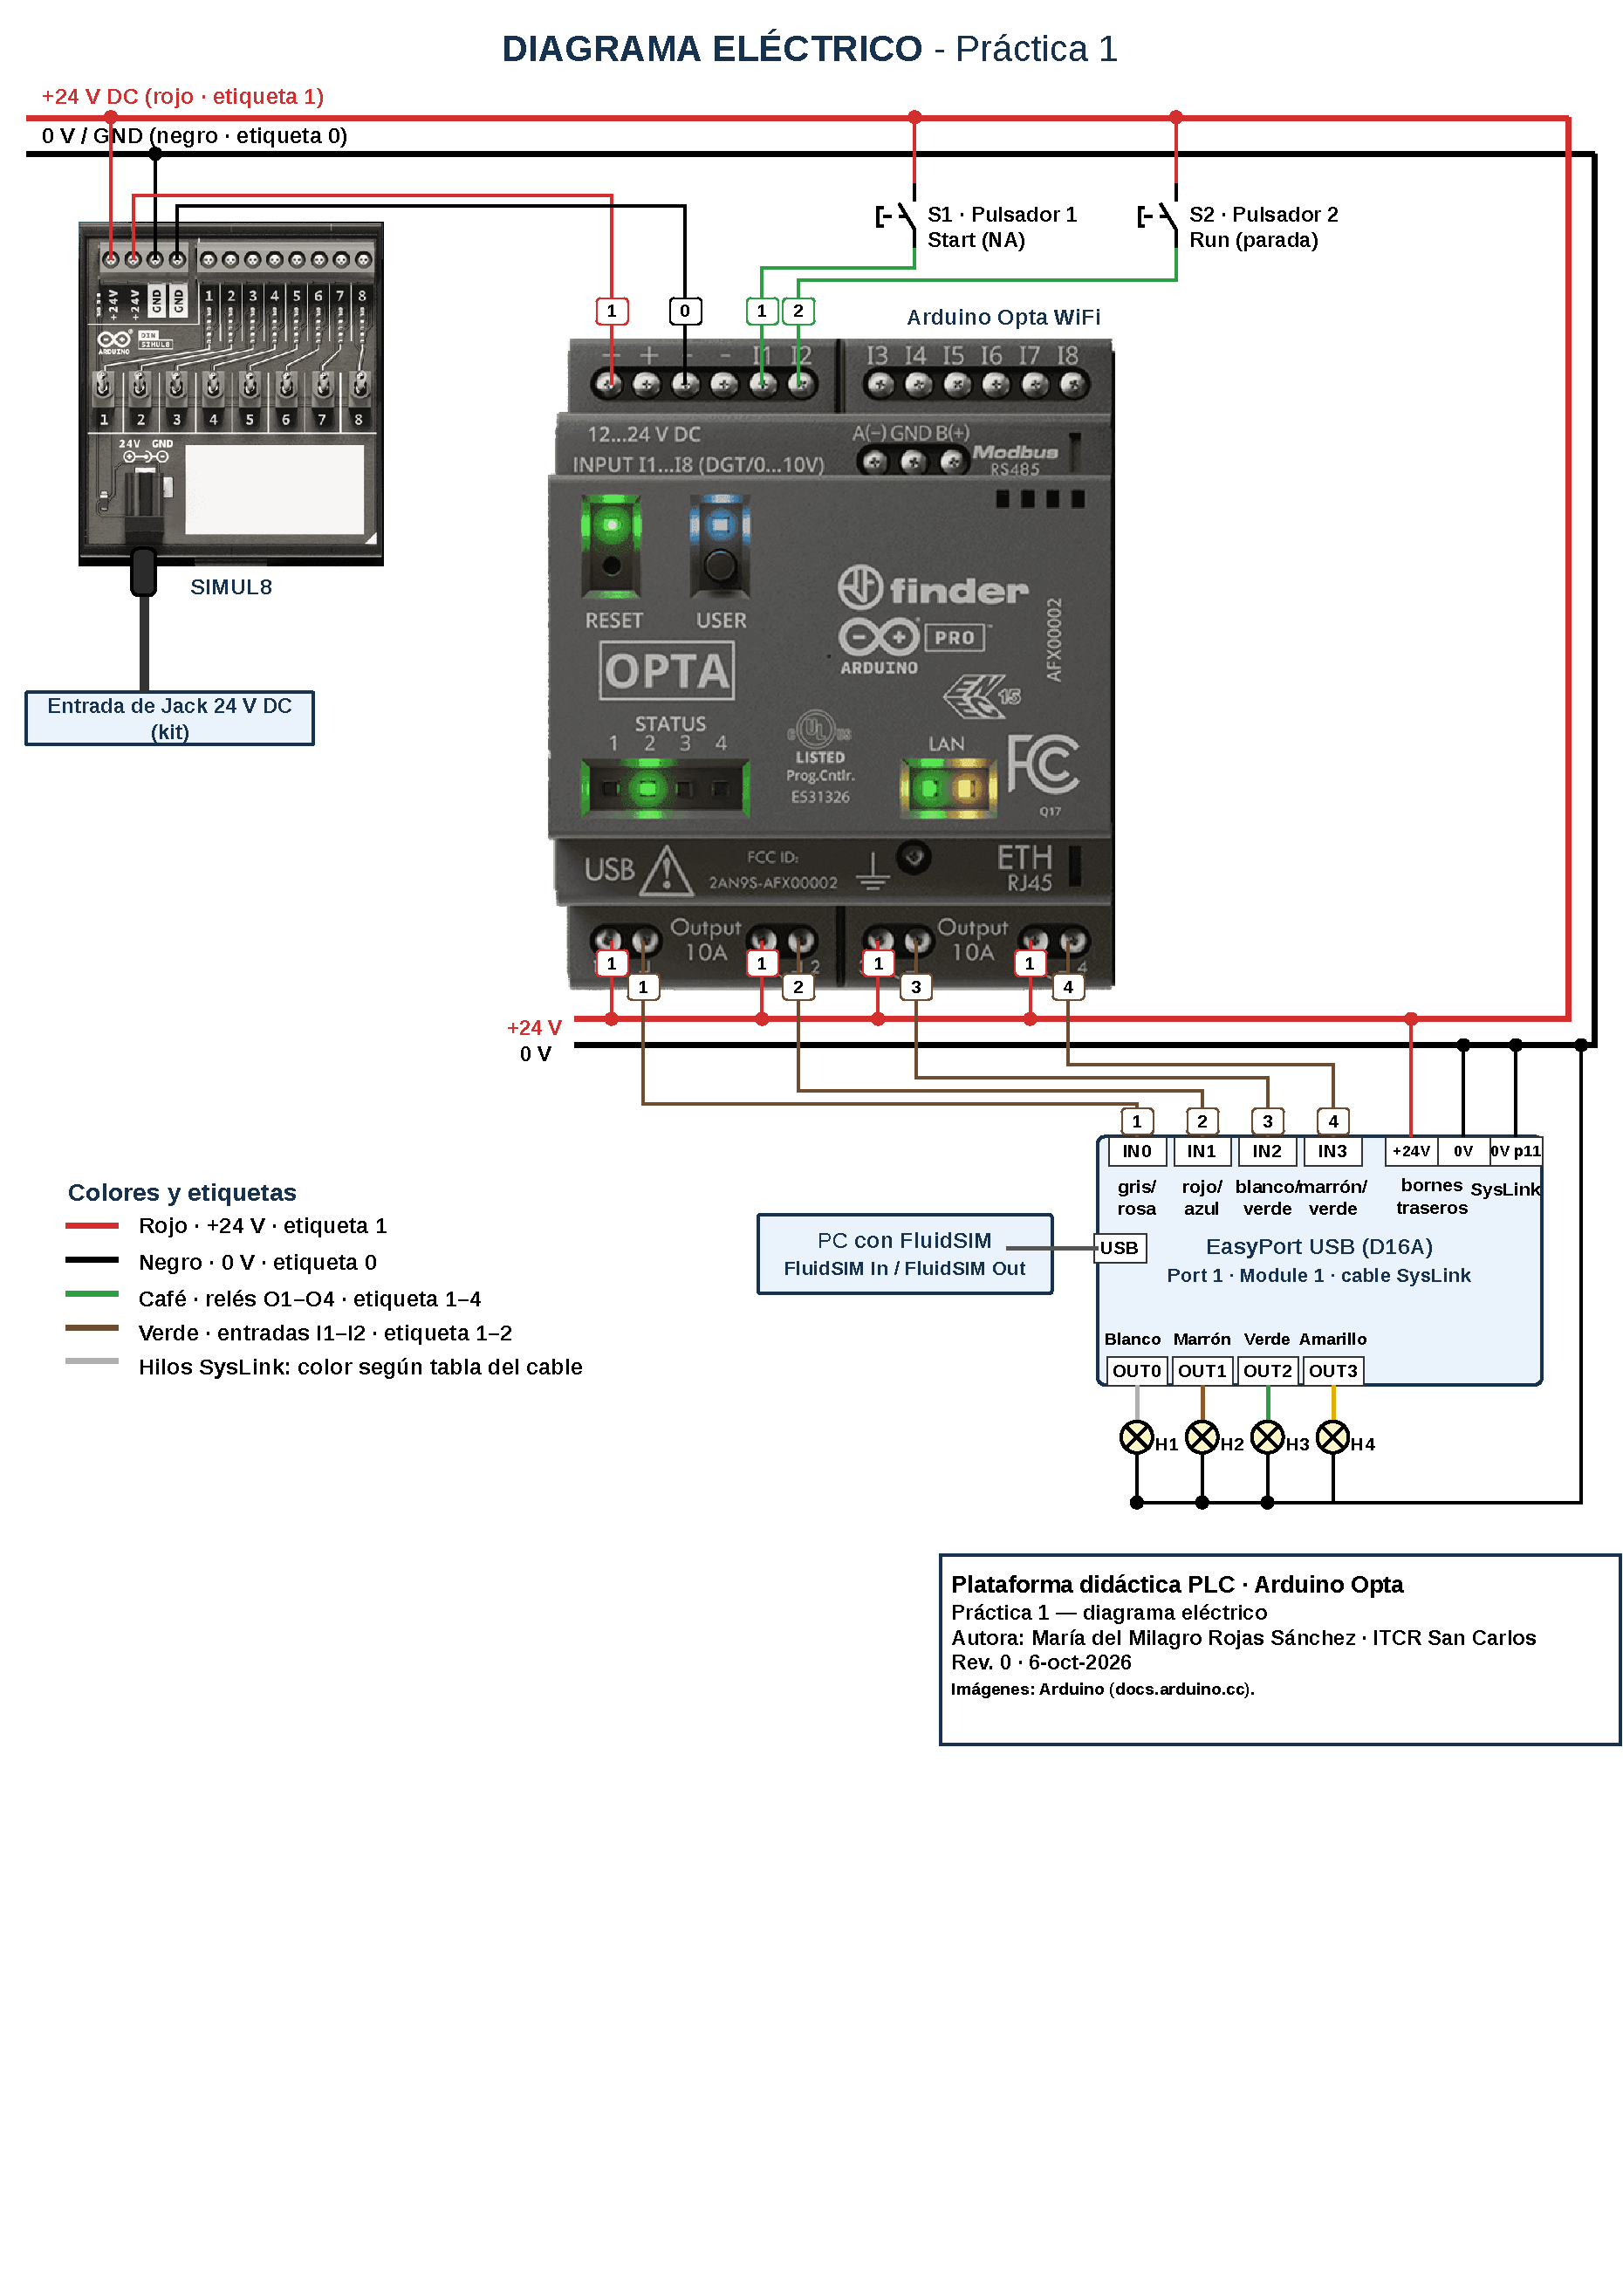
\includegraphics[width=0.9\textwidth,trim=6 290 0 8,clip]{Diagrama_Electrico_Practica1.pdf}
    \caption{Diagrama eléctrico de las conexiones usadas en la Práctica~1. Fuente: Autora.}
    \label{fig:diagrama_p1}
\end{figure}

% -------------------------------------------------
\subsection{Práctica 2: sistema de enfriamiento con ventilación regulable}
\label{subsec:res_p2}
% -------------------------------------------------

\textbf{Objetivo.} Simular un recinto que se calienta y un ventilador cuya velocidad se ajusta según la temperatura. El DIN Celsius representa el recinto, pues su sensor mide la temperatura y sus dos calentadores, que se encienden y apagan con pulsadores, representan las cargas que aportan calor. La salida del controlador regula el motor del ventilador por PWM y se entrega además como tensión de 0 a 10~V hacia el EasyPort.

\textbf{Materiales.} Plataforma didáctica con el Arduino Opta WiFi y la expansión A0602, DIN Celsius, DIN Simul8 como pulsadores, motor de corriente continua de 24~V y 0,5~A como ventilador, EasyPort USB, multímetro y computador con PLC IDE y Festo EasyPort Web Bridge.

\textbf{Resultados.} El programa de la Figura~\ref{fig:flujo_p2} se ejecutó en una tarea periódica de 50~ms. La Tabla~\ref{tab:resultados_temperatura} reúne las temperaturas leídas en las dos condiciones de prueba: a temperatura ambiente, la lectura convertida con la Ecuación~(\ref{eq:temp}) estuvo entre 26 y 29~$^\circ$C, y con los dos calentadores encendidos la placa llegó a 45--47~$^\circ$C. En ese rango la salida del controlador siguió la Ecuación~(\ref{eq:control}), desde 0~\% por debajo de 28~$^\circ$C hasta más de 90~\%, y el motor varió su velocidad en consecuencia.

\begin{table}[H]
\centering
\caption{Temperaturas leídas en la Práctica~2 y salida del controlador correspondiente según la Ecuación~(\ref{eq:control}), con $K_P = 5$ y $T_{\mathrm{ref}} = 28~^\circ$C. Fuente: Autora.}
\label{tab:resultados_temperatura}
\renewcommand{\arraystretch}{1.3}
\begin{tabularx}{\textwidth}{|X|p{3.4cm}|p{3.4cm}|}
\hline
\filacolor{TableGray}
\textbf{Condición de prueba} & \textbf{Temperatura leída [$^\circ$C]} & \textbf{Salida del controlador [\%]} \\
\hline
Temperatura ambiente, calentadores apagados & 26--29 & 0--5 \\
\hline
Dos calentadores encendidos & 45--47 & 85--95 \\
\hline
\end{tabularx}
\end{table}

La escala de la salida analógica se obtuvo midiendo con el multímetro la tensión del borne \texttt{O1} respecto de GND para valores fijos del convertidor (Tabla~\ref{tab:resultados_dac}), y la misma tensión se leyó en el EasyPort. La práctica valida la entrada analógica, la salida PWM, la salida analógica y el cálculo con números reales en el controlador; también evidenció la necesidad de actualizar el \emph{firmware} de la expansión para habilitar las salidas PWM. La Figura~\ref{fig:diagrama_p2} muestra las conexiones usadas.

\begin{table}[H]
\centering
\caption{Tensión medida en la salida analógica \texttt{O1} del A0602 para valores fijos del convertidor (Práctica~2). Fuente: Autora.}
\label{tab:resultados_dac}
\renewcommand{\arraystretch}{1.3}
\begin{tabularx}{\textwidth}{|X|X|X|}
\hline
\filacolor{TableGray}
\textbf{Valor escrito [cuentas]} & \textbf{Tensión medida [V]} & \textbf{Relación [mV/cuenta]} \\
\hline
0 & 0 & -- \\
\hline
4000 & 5,9 & 1,475 \\
\hline
8000 & 11,8 & 1,475 \\
\hline
\end{tabularx}
\end{table}

\begin{figure}[H]
    \centering
    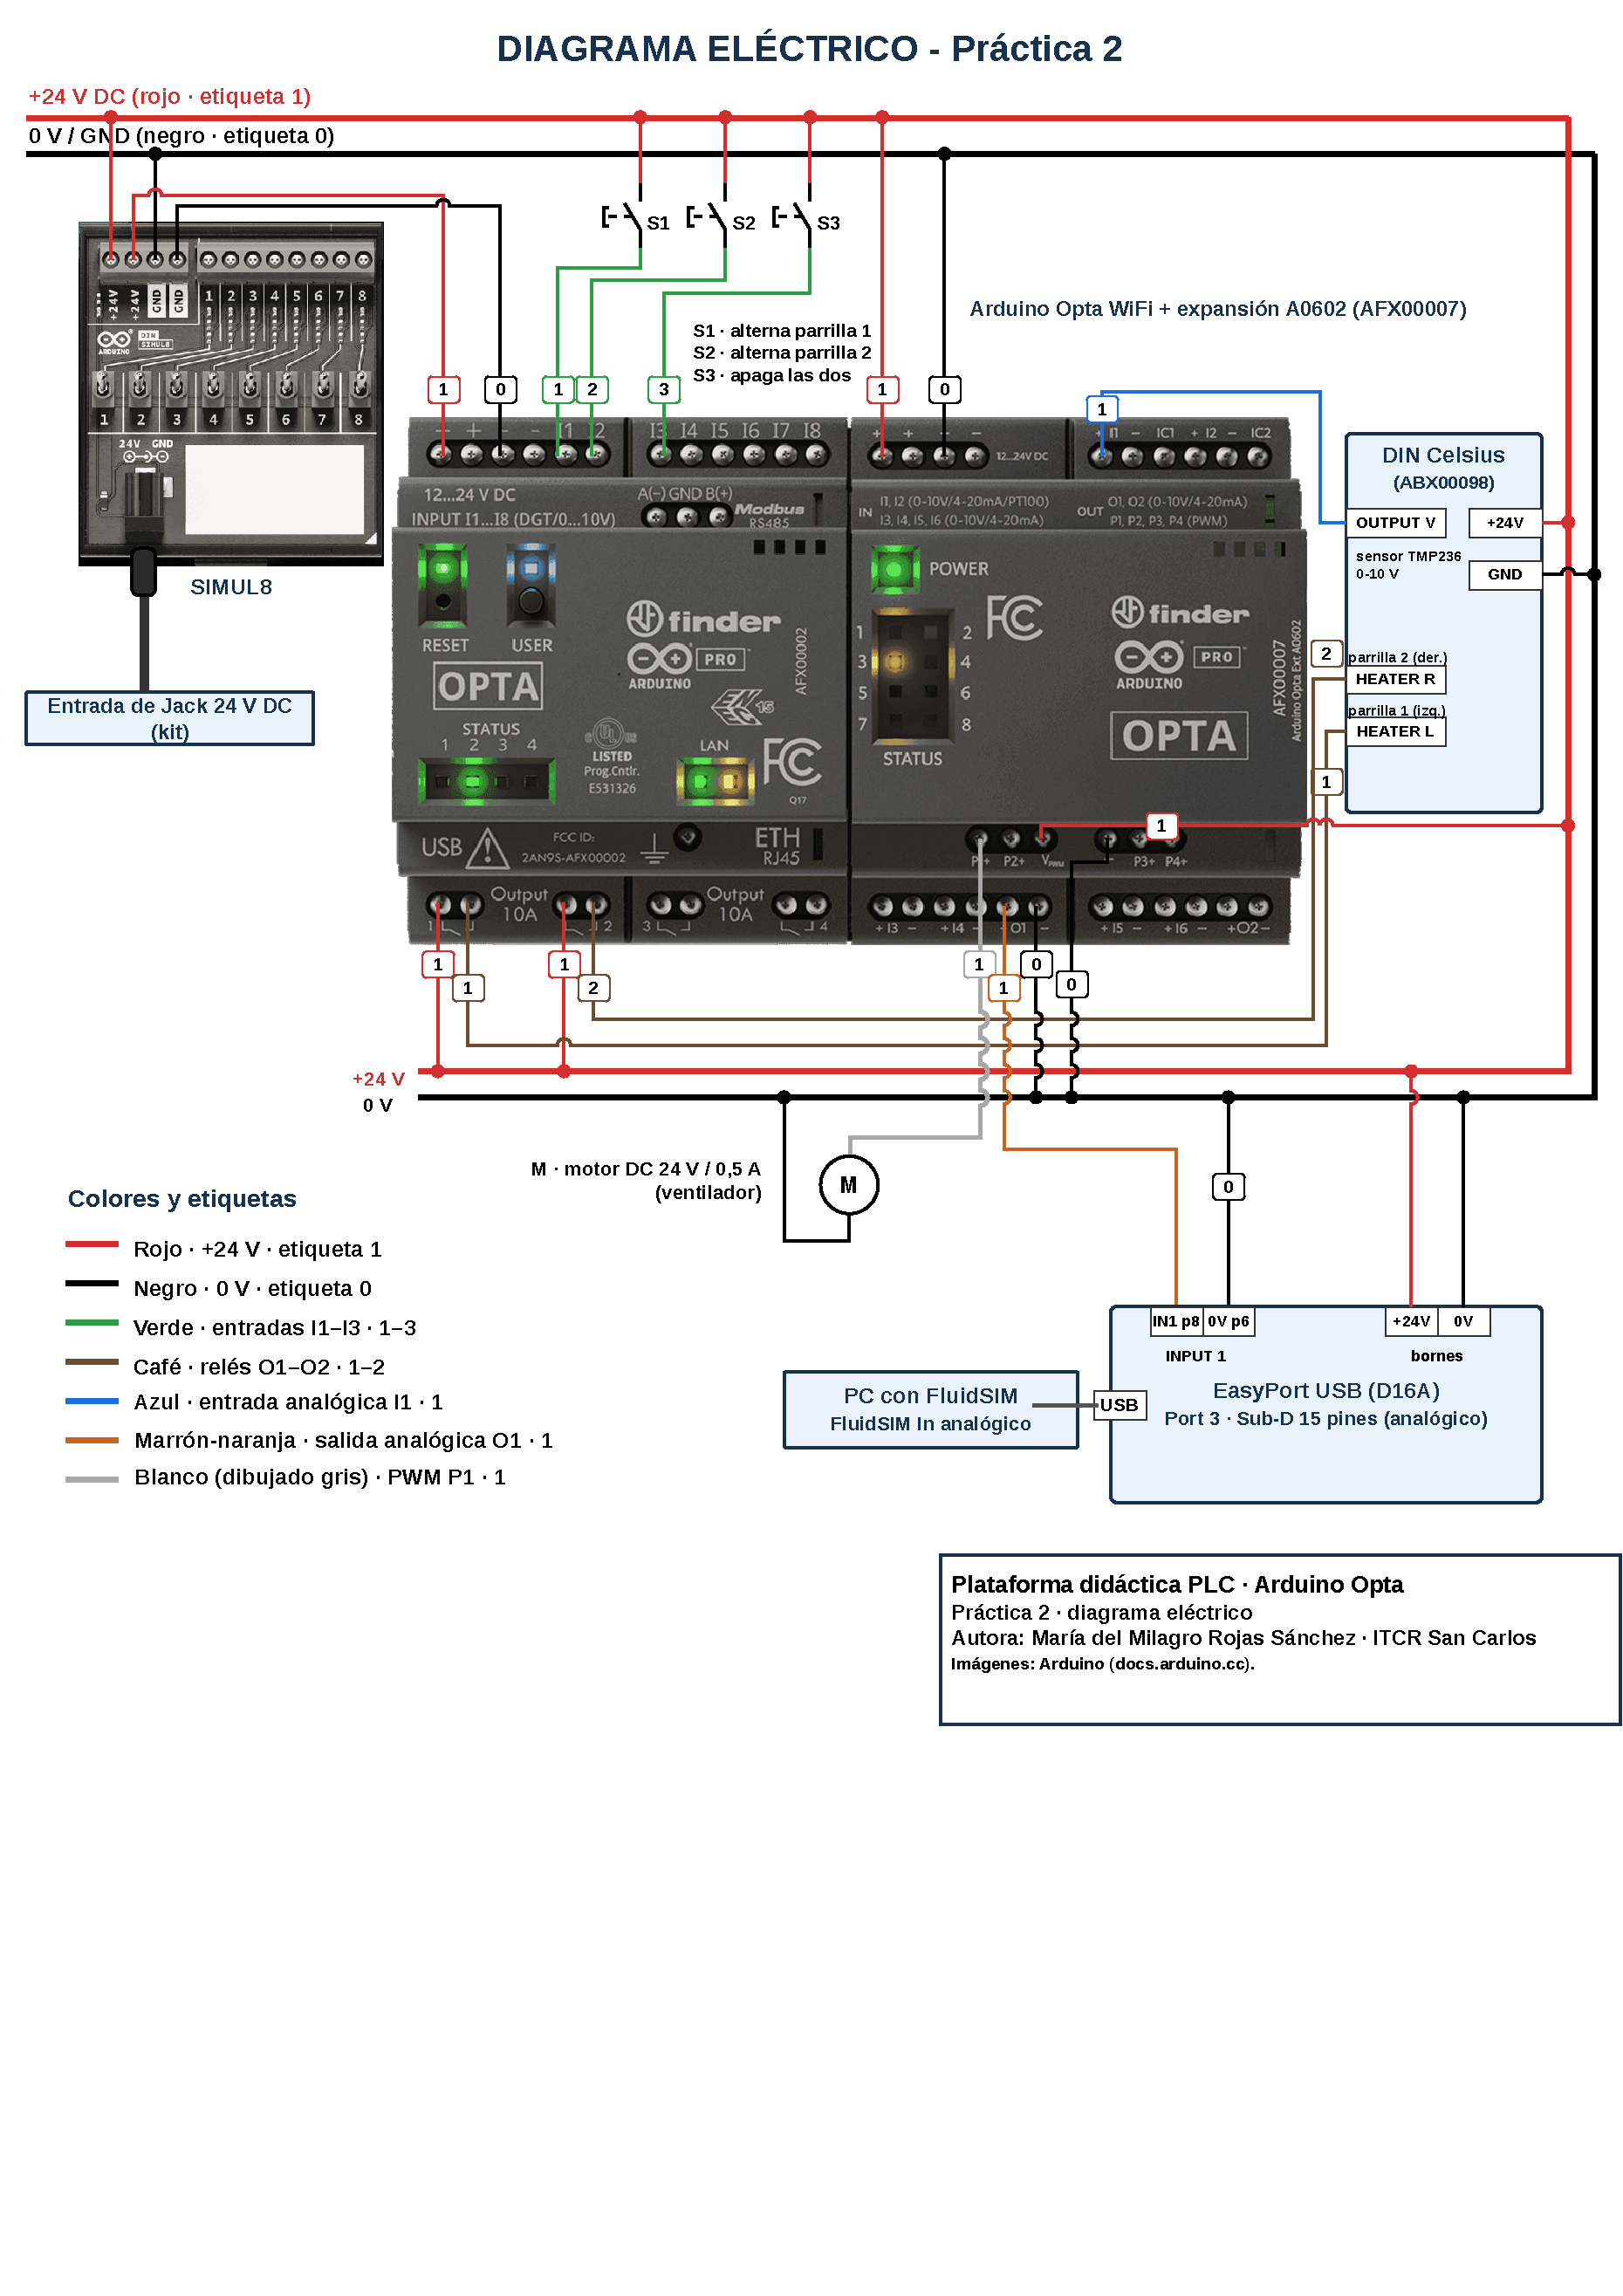
\includegraphics[width=0.9\textwidth,trim=6 290 0 8,clip]{Diagrama_Electrico_Practica2.pdf}
    \caption{Diagrama eléctrico de las conexiones usadas en la Práctica~2. Fuente: Autora.}
    \label{fig:diagrama_p2}
\end{figure}

% -------------------------------------------------
\section{Análisis}
\label{sec:analisis}
% -------------------------------------------------

Los resultados se analizan a continuación frente a cada objetivo específico, y luego frente a los alcances y limitaciones que se fijaron para el proyecto en las Secciones~\ref{sec:alcances} y~\ref{sec:limitaciones}.

\subsection{Panel de control (objetivo específico 1)}

El panel integra el Arduino Opta y la expansión A0602 sobre riel DIN y deja a la vista del usuario toda la plataforma; las conexiones de los dispositivos de campo se concentran en la regleta del riel~3, ordenada en ocho grupos rotulados que siguen la secuencia de entradas y salidas del sistema (Sección~\ref{subsec:hw_terminales}). El cableado interno sigue el código de colores por tipo de señal de la Tabla~\ref{tab:codigo_colores}, con una etiqueta numérica por canal, y las borneras de alimentación X24V y X0V quedan en el riel~2, separadas de la regleta de señales y con su propio color y etiqueta (rojo con 1 y negro con 0). Se verificó la continuidad de todas las conexiones y, a partir del cableado ya verificado, se elaboró el diagrama eléctrico general del sistema (Figura~\ref{fig:diagrama_electrico}). En las dos prácticas, los dispositivos de campo se conectaron sobre la regleta, que es la condición de operación que el objetivo busca garantizar.

\subsection{Verificación de señales (objetivo específico 2)}

La Tabla~\ref{tab:cobertura_senales} relaciona cada tipo de señal de la plataforma con el dispositivo de bajo costo con que se probó y la práctica en que se verificó. Entre las dos prácticas quedaron validados los cinco tipos de señal que la plataforma ofrece al estudiante, lo que cumple el segundo indicador del objetivo; el primero se cumple con la guía de laboratorio, que desarrolla ambas prácticas paso a paso y combina la plataforma física con la planta virtual de FluidSIM.

\begin{table}[H]
\centering
\caption{Tipos de señal verificados en las prácticas y dispositivo de prueba empleado. Fuente: Autora.}
\label{tab:cobertura_senales}
\footnotesize
\renewcommand{\arraystretch}{1.3}
\renewcommand\tabularxcolumn[1]{m{#1}}
\begin{tabularx}{\textwidth}{|>{\raggedright\arraybackslash}m{2.9cm}|>{\raggedright\arraybackslash}m{2.6cm}|>{\raggedright\arraybackslash}X|>{\centering\arraybackslash}m{1.7cm}|}
\hline
\filacolor{TableGray}
\textbf{Tipo de señal} & \textbf{Grupo de la regleta} & \textbf{Dispositivo de prueba} & \textbf{Práctica} \\
\hline
Entrada digital de 24~V & Entradas digitales del Opta (X3) & Pulsadores de 24~V e interruptores del DIN Simul8 & 1 y 2 \\
\hline
Salida de relé & Salidas de relé del Opta (X4) & Entradas del EasyPort hacia los cilindros simulados en FluidSIM; calentadores del DIN Celsius & 1 y 2 \\
\hline
Entrada analógica de 0--10~V & Entradas analógicas del A0602 (X5) & Sensor TMP236 del DIN Celsius & 2 \\
\hline
Salida PWM & Salida \texttt{P1} del A0602 (X7) & Motor de corriente continua de 24~V & 2 \\
\hline
Salida analógica de 0--10~V & Salida \texttt{O1} del A0602 (X6) & Multímetro y entrada analógica del EasyPort & 2 \\
\hline
\end{tabularx}
\end{table}

Los resultados de la Práctica~2 confirman además los criterios de diseño del Capítulo~\ref{chp:enfoque}:

\begin{itemize}
    \item \textbf{Lectura de temperatura.} La dispersión de las lecturas a temperatura ambiente (26 a 29~$^\circ$C) es del orden de la exactitud del sensor, $\pm$2,5~$^\circ$C~\cite{ref37}, por lo que la conversión de la Ecuación~(\ref{eq:temp}) es coherente con los datos del fabricante.
    \item \textbf{Ganancia del controlador.} Con $K_P = 5$ y $T_{\mathrm{ref}} = 28~^\circ$C, la salida se satura en 100~\% a 48~$^\circ$C, apenas por encima de la temperatura máxima que alcanzaron los calentadores (47~$^\circ$C). La ganancia elegida aprovecha así casi todo el recorrido de la salida PWM sin llegar a saturarla dentro del rango de la práctica.
    \item \textbf{Salida analógica.} Los dos puntos medidos dan la misma relación, 1,475~mV por cuenta, de modo que la salida es lineal y pasa por el origen; una sola constante de escala (67,8 cuentas por punto porcentual) basta para que el 100~\% de la salida del controlador corresponda a 10~V.
    \item \textbf{Alimentación.} La práctica operó la configuración más exigente del balance de la Tabla~\ref{tab:balance_potencia}, con los dos calentadores y el motor funcionando a la vez, con el adaptador de 1~A del kit como única fuente.
    \item \textbf{\emph{Firmware} de la expansión.} Con la versión 0.1.4 de fábrica, la salida PWM no respondía; la actualización a la 0.1.14 fue condición para completar la práctica, y es un paso que cualquier unidad nueva debe repetir.
\end{itemize}

\subsection{Costo-beneficio (objetivo específico 3)}

Los dos indicadores del objetivo se cumplen en la Sección~\ref{sec:costo_beneficio}. La Tabla~\ref{tab:costo_beneficio} compara los costos con precios de referencia documentados. Un puesto con S7-1500 cuesta unas 3,6 veces la plataforma en hardware y unas 9,5 veces con la licencia de programación, y el equipo base del EduTrainer, unas 11 veces. La Tabla~\ref{tab:equivalencia_tecnica} muestra que, en lo que exige un curso de programación de PLC (lenguajes de IEC~61131-3, señales a 24~V~DC, comunicación y ampliación modular), la plataforma es funcionalmente comparable a ambos sistemas. Los montos están sujetos al tipo de cambio y a la vigencia de cada cotización, por lo que las relaciones, más que las cifras absolutas, son el resultado a retener.

\subsection{Alcances y limitaciones de la solución implementada}

La plataforma cubrió los alcances de diseño del panel, integración del hardware, verificación experimental, análisis costo-beneficio y programación de lógicas de demostración. Algunos elementos no se ejercitaron en las prácticas reportadas:

\begin{itemize}
    \item La tarjeta optoacopladora PC817 se verificó en banco antes del montaje (Sección~\ref{subsec:hw_opto}), pero ninguna de las dos prácticas la usa con un circuito propio del estudiante.
    \item El sensor de proximidad inductivo seleccionado no forma parte de las prácticas.
    \item Las entradas del A0602 se probaron solo en modo de tensión de 0--10~V; los modos de 4--20~mA y RTD no se ensayaron.
\end{itemize}

Ambas prácticas se programaron en Ladder Diagram, por ser el lenguaje más extendido en la industria (Sección~\ref{sec:iec}); FBD y ST se cubren mediante los tutoriales introductorios oficiales de Arduino que la guía enlaza en su sección inicial (Apéndice~\ref{chp:guia}), conforme al alcance de programación definido en la Sección~\ref{sec:alcances}.

Las limitaciones fijadas en la Sección~\ref{sec:limitaciones} se mantienen: la comunicación Modbus se documentó sin cablearse, la plataforma es una unidad prototipo y la verificación fue funcional, sin un estudio del impacto en el aprendizaje de los estudiantes. En cuanto a la meta del proyecto, la plataforma y su guía quedan listas para incorporarse a los cursos de la carrera; su uso con estudiantes está previsto para los próximos cursos.

% =================================================================
\chapter{Conclusiones y recomendaciones}
\label{chp:conclusiones}
% =================================================================

Este capítulo reúne las conclusiones del proyecto y las recomendaciones para usar la plataforma, reproducirla en nuevos puestos de trabajo y ampliar su uso.

% -------------------------------------------------
\section{Conclusiones}
% -------------------------------------------------

\begin{itemize}
    \item Se diseñó y montó una plataforma didáctica modular basada en el Arduino Opta WiFi que permite ejecutar prácticas completas de programación PLC con lenguajes IEC~61131-3 y señales industriales a 24~V~DC.
    \item El panel de control deja a la vista toda la plataforma y concentra las conexiones del estudiante en una regleta de ocho grupos rotulados, con código de colores y etiquetas por tipo de señal y con la alimentación separada de las señales, lo que evita cablear directamente sobre los bornes del hardware de control.
    \item Las dos prácticas, programadas en Ladder Diagram por ser el lenguaje más extendido en la industria, validaron con dispositivos de bajo costo los cinco tipos de señal de la plataforma (entrada digital, salida de relé, entrada analógica, salida analógica y salida PWM), y la guía de laboratorio las documenta paso a paso.
    \item Un puesto convencional con S7-1500 y licencia cuesta unas 9,5 veces la plataforma, y el equipo base del EduTrainer unas 11 veces, con funcionalidad comparable para la enseñanza de programación de PLC; además, el entorno de programación gratuito permite replicar la plataforma sin gasto en licencias.
    \item La plataforma se adapta a equipos didácticos de otros fabricantes, como el EasyPort de Festo, y a entornos virtuales como FluidSIM, de modo que el controlador real puede gobernar procesos simulados que no existen físicamente en el laboratorio, lo que extiende los alcances didácticos de las prácticas.
    \item La plataforma y su guía de laboratorio permiten que los cursos de la carrera incorporen prácticas con un PLC real, sin depender de equipo industrial de alto costo.
    \item La plataforma queda equipada con una tarjeta optoacopladora de cuatro canales aislados, cuyo lado de salida se alimenta con la fuente del circuito del estudiante y se adapta a la tensión que este requiera (de 3,6 a 30~V), de modo que las salidas del PLC pueden gobernar circuitos electrónicos propios y unir la automatización a 24~V~DC con lo que el estudiante construye en los demás laboratorios de la carrera.
\end{itemize}

% -------------------------------------------------
\section{Recomendaciones}
% -------------------------------------------------

\begin{itemize}
    \item Cotizar de nuevo el kit AKX00051, el módulo AFX00007 y los materiales antes de cada réplica, ya que los montos del presupuesto (Apéndice~\ref{chp:presupuesto}) dependen del tipo de cambio y de la vigencia de las cotizaciones.
    \item Reutilizar el plan de corte de seis perfiles y los modelos de las piezas de unión (Sección~\ref{subsec:hw_estructura}), e imprimir las piezas en ABS, por ser un material más resistente y de mayor confiabilidad que el PLA.
    \item Si alguna de las piezas de unión impresas de la plataforma actual se daña, reemplazarla por la misma pieza impresa en ABS.
    \item Cablear cada unidad con el código de colores y las etiquetas de la Tabla~\ref{tab:codigo_colores}, tomando como referencia el diagrama de la Figura~\ref{fig:diagrama_electrico}, y verificar la continuidad de cada conexión antes de energizar.
    \item Alimentar el A0602 desde las borneras X24V y X0V, porque no recibe energía por el bus AUX, y actualizar su \emph{firmware} a la versión 0.1.8 o superior antes del primer uso.
   
    \item Retirar los cuatro puentes de tierra de la tarjeta PC817 para conservar el aislamiento entre canales y respecto del 0~V del panel.
    \item Medir de nuevo la escala de la salida analógica en cada unidad, con el multímetro y dos o tres valores fijos del convertidor, en lugar de copiar la constante de 67,8 cuentas por punto porcentual.
    \item Respetar el margen de unos 0,3~A del adaptador y alimentar con una fuente externa, conmutada por los relés, cualquier carga que lo supere.
    \item Mantener sensores de salida PNP; un sensor NPN exige una resistencia de polarización hacia +24~V en cada entrada.
  
  
    \item Al incorporar la plataforma en los cursos de la carrera, como está previsto, evaluar su efecto en el aprendizaje, para obtener la validación pedagógica que quedó fuera del alcance.
    \item Incorporar elementos de sujeción en caso de requerir transportar el equipo entre aulas.
\end{itemize}

% =================================================================
% BIBLIOGRAFÍA
% =================================================================
\begin{thebibliography}{99}
\addcontentsline{toc}{chapter}{\bibname}

\bibitem{ref1}
Arduino, ``Opta: Hardware Documentation,'' \emph{Arduino Documentation}. [En línea]. Disponible en: \url{https://docs.arduino.cc/hardware/opta/}. [Accedido: 20-mar-2026].

\bibitem{ref2}
Arduino Education, ``PLC Starter Kit,'' \emph{Arduino}. [En línea]. Disponible en: \url{https://www.arduino.cc/education/plc-starter-kit}. [Accedido: 20-mar-2026].

\bibitem{ref3}
M. A. Koondhar, G. S. Kaloi, A. K. Junejo, A. H. Soomro, S. Chandio y M. Ali, ``The Role of PLC in Automation, Industry and Education Purpose: A Review,'' \emph{Pakistan Journal of Engineering, Technology \& Science}, vol.~11, no.~2, pp.~22--31, 2023.

\bibitem{ref4}
J. L. Vázquez-González, J. Barrios-Avilés, A. Rosado-Muñoz y R. Alejos-Palomares, ``An Industrial Automation Course: Common Infrastructure for Physical, Virtual and Remote Laboratories for PLC Programming,'' \emph{International Journal of Online Engineering (iJOE)}, vol.~14, no.~8, pp.~4--19, 2018, doi: 10.3991/ijoe.v14i08.8758.

\bibitem{ref5}
O. G. Bellmunt, D. M. Miracle, S. G. Arellano, A. Sumper y A. S. Andreu, ``A Distance PLC Programming Course Employing a Remote Laboratory Based on a Flexible Manufacturing Cell,'' \emph{IEEE Transactions on Education}, vol.~49, no.~2, pp.~278--284, 2006, doi: 10.1109/TE.2006.873982.

\bibitem{ref6}
A. Liljaniemi y H. Paavilainen, ``Using Digital Twin Technology in Engineering Education: Course Concept to Explore Benefits and Barriers,'' \emph{Open Engineering}, vol.~10, no.~1, pp.~377--385, 2020, doi: 10.1515/eng-2020-0040.

\bibitem{ref7}
ControlByte, ``Siemens SIMATIC S7-1200 PLC Controller: Learn the Basics,'' \emph{ControlByte Blog}. [En línea]. Disponible en: \url{https://controlbyte.tech/blog/siemens-simatic-s7-1200-plc-controller-learn-the-basics/}. [Accedido: 18-abr-2026]. [Imagen ilustrativa].

\bibitem{ref8}
Arduino, ``Opta User Manual,'' \emph{Arduino Documentation}. [En línea]. Disponible en: \url{https://docs.arduino.cc/tutorials/opta/user-manual/}. [Accedido: 18-abr-2026]. [Imágenes ilustrativas].

\bibitem{ref9}
Unsplash, ``Producción en línea de montaje de automóviles: brazo robótico en línea de producción,'' \emph{Unsplash}. [En línea]. Disponible en: \url{https://unsplash.com/photos/o4exhQKCbRE}. [Accedido: 18-abr-2026]. [Imagen ilustrativa].

\bibitem{ref10}
M. Al-Yaman, D. Alswaiti, A. Alsharkawi y M. Al-Taee, ``A cost-effective modular laboratory
solution for industrial automation and applied engineering education,'' \emph{MethodsX},
vol.~14, art.~103388, 2025, doi: 10.1016/j.mex.2025.103388.

\bibitem{ref11}
H. Vargas, R. Heradio, M. Donoso y G. Farias, ``Teaching automation with Factory~I/O under a
competency-based curriculum,'' \emph{Multimedia Tools and Applications}, vol.~82,
pp.~19221--19246, 2023, doi: 10.1007/s11042-022-14047-9.

\bibitem{ref12}
C.~A. Anguiano-Gijón et al., ``Simulation of a sequential system using the S7-1200 platform
and touch panel KTP700 in the context of technical education,'' \emph{Procedia Computer
Science}, 2024. [En línea]. Disponible en:
\url{https://www.sciencedirect.com/science/article/pii/S1877050924023743}.
[Accedido: 25-jun-2026].

\bibitem{ref13}
CRCibernética, ``PC817 Optocoupler Board,'' \emph{CRCibernética}. [En línea]. Disponible en:
\url{https://www.crcibernetica.com/pc817-optocoupler-board/}. [Accedido: 1-set-2026].

\bibitem{ref14}
Sharp Corporation, ``PC817 Series: High Density Mounting Type Photocoupler,'' hoja de datos.
[En línea]. Disponible en:
\url{https://www.learnabout-electronics.org/Downloads/PC817\%20optocoupler.pdf}.
[Accedido: 1-set-2026].

\bibitem{ref15}
CRCibernética, ``Optocoupler MOSFET Driver Module,'' \emph{CRCibernética}. [En línea]. Disponible en:
\url{https://www.crcibernetica.com/optocoupler-mosfet-driver-module/}. [Accedido: 1-set-2026].

\bibitem{ref16}
CRCibernética, ``4N25 DIP-6 Optocoupler,'' \emph{CRCibernética}. [En línea]. Disponible en:
\url{https://www.crcibernetica.com/4n25-dip-6-optocoupler/}. [Accedido: 1-set-2026].

\bibitem{ref17}
Relepro, ``Siemens SIMATIC S7-1500 CPU 1513-1 PN (6ES7513-1AL02-0AB0),'' \emph{Relepro}. [En línea].
Disponible en:
\url{https://relepro.com/cpu-1500-estandar/327/siemens_s7-1500-cpu-1513-1-pn_6es7513-1al02-0ab0.html}.
[Accedido: 7-set-2026]. [Imagen ilustrativa].

\bibitem{ref18}
Festo, ``Opciones preferidas de EduTrainer Universal para laboratorio con SIMATIC S7-1500,''
\emph{Festo}. [En línea]. Disponible en:
\url{https://www.festo.com/mx/es/p/opciones-preferidas-de-edutrainer-universal-para-laboratorio-con-simatic-s7-1500-id_PROD_DID_8034574}.
[Accedido: 7-set-2026]. [Imagen ilustrativa].

\bibitem{ref19}
MicroJPM, ``Arduino UNO R3 [versión genérica], AD20477,'' \emph{MicroJPM}. [En línea]. Disponible en:
\url{https://www.microjpm.store/products/ad20477}. [Accedido: 7-set-2026]. [Imagen ilustrativa].

\bibitem{ref20}
MicroJPM, ``ESP-32 Development Board 2.4 GHz Dual-Mode WiFi + Bluetooth, AD42922,'' \emph{MicroJPM}.
[En línea]. Disponible en:
\url{https://www.microjpm.store/products/ad42922}. [Accedido: 7-set-2026]. [Imagen ilustrativa].

\bibitem{ref21}
Twidec, ``M12 Approach Sensor Inductive Proximity Switch PNP NO, DC 6--36~V, 4~mm,
LJ12A3-4-Z/BY,'' \emph{Amazon}. [En línea]. Disponible en:
\url{https://www.amazon.com/dp/B07NYD3CPK}. [Accedido: 7-set-2026]. [Imagen ilustrativa].

\bibitem{ref22}
``LJC18A3-B-Z/BY Capacitive Proximity Sensor Switch, tres hilos, PNP NO, 10~mm, DC 6--36~V,''
\emph{Amazon}. [En línea]. Disponible en:
\url{https://www.amazon.com/dp/B0C4XBNJZF}. [Accedido: 7-set-2026]. [Imagen ilustrativa].

\bibitem{ref23}
OMRON Corporation, ``Proximity Sensors: Technical Guide,'' \emph{OMRON Industrial Automation}.
[En línea]. Disponible en: \url{https://www.ia.omron.com/support/guide/41/introduction.html}.
[Accedido: 7-set-2026].

\bibitem{ref24}
CRCibernética, ``SN04N Proximity Switch 10--30V,'' \emph{CRCibernética}. [En línea]. Disponible en:
\url{https://www.crcibernetica.com/sn04n-proximity-switch-10-30v/}. [Accedido: 7-set-2026].
[Imagen ilustrativa].

\bibitem{ref25}
Gebildet, ``5pcs 10mm AC/DC 12--24V LED Metal Indicator Light Waterproof Signal Lamp with Wire,''
\emph{Amazon}. [En línea]. Disponible en: \url{https://www.amazon.com/dp/B08LDCQR9D}.
[Accedido: 7-set-2026]. [Imagen ilustrativa].

\bibitem{ref26}
Gebildet, ``5pcs 12mm 2A 12V/24V/125V/250V AC Prewired Waterproof Momentary Stainless Steel Push
Button,'' \emph{Amazon}. [En línea]. Disponible en: \url{https://www.amazon.com/dp/B08L49F7DV}.
[Accedido: 7-set-2026]. [Imagen ilustrativa].

\bibitem{ref27}
Festo Didactic SE, \emph{EasyPort USB: Manual}, ref.\ 721876, ed.\ 10/2011, Denkendorf, Alemania, 2011.

\bibitem{ref28}
Festo, ``Simulation software FluidSIM,'' \emph{Festo}. [En línea]. Disponible en:
\url{https://www.festo.com/us/en/e/technical-education/digital-learning/virtual-simulation-and-modeling/fluidsim-id_1663056}.
[Accedido: 29-set-2026].

\bibitem{ref29}
B. Dannegård y T. Chung, ``Getting Started with RS-485 on Opta,'' \emph{Arduino Documentation}. [En línea]. Disponible en: \url{https://docs.arduino.cc/tutorials/opta/getting-started-with-rs485/}. [Accedido: 21-oct-2026].

\bibitem{ref30}
J. Bagur y T. Chung, ``Getting Started with Modbus RTU on Opta,'' \emph{Arduino Documentation}. [En línea]. Disponible en: \url{https://docs.arduino.cc/tutorials/opta/getting-started-with-modbus-rtu/}. [Accedido: 21-oct-2026]. [Imágenes ilustrativas].

\bibitem{ref31}
Modbus Organization, \emph{MODBUS over Serial Line: Specification and Implementation Guide}, V1.02, 2006. [En línea]. Disponible en: \url{https://www.modbus.org/file/secure/modbusoverserial.pdf}. [Accedido: 21-oct-2026].

\bibitem{ref32}
Modbus Organization, \emph{MODBUS Application Protocol Specification}, V1.1b3, 2012. [En línea]. Disponible en: \url{https://www.modbus.org/file/secure/modbusprotocolspecification.pdf}. [Accedido: 21-oct-2026].

\bibitem{ref33}
T. Chung y J. Bagur, ``Modbus RTU On Opta Using PLC IDE,'' \emph{Arduino Documentation}. [En línea]. Disponible en: \url{https://docs.arduino.cc/tutorials/opta/opta-modbus-rtu-plc-ide/}. [Accedido: 21-oct-2026].

\bibitem{ref34}
Arduino, ``Arduino Opta: Product Reference Manual (AFX00001, AFX00002, AFX00003),'' hoja de datos. [En línea]. Disponible en: \url{https://docs.arduino.cc/resources/datasheets/AFX00001-AFX00002-AFX00003-datasheet.pdf}. [Accedido: 26-oct-2026].

\bibitem{ref35}
Arduino, ``Arduino Opta Analog Expansion: Product Reference Manual (AFX00007),'' hoja de datos. [En línea]. Disponible en: \url{https://docs.arduino.cc/resources/datasheets/AFX00007-datasheet.pdf}. [Accedido: 26-oct-2026].

\bibitem{ref36}
Arduino, ``Arduino PLC Starter Kit: Product Reference Manual (AKX00051),'' hoja de datos. [En línea]. Disponible en: \url{https://docs.arduino.cc/resources/datasheets/AKX00051-datasheet.pdf}. [Accedido: 26-oct-2026].

\bibitem{ref37}
Arduino, ``Arduino DIN Celsius: Product Reference Manual (ABX00098),'' hoja de datos. [En línea]. Disponible en: \url{https://docs.arduino.cc/resources/datasheets/ABX00098-datasheet.pdf}. [Accedido: 26-oct-2026].

\bibitem{ref38}
International Electrotechnical Commission, \emph{IEC 61131-3: Programmable controllers. Part 3: Programming languages}, 3.ª ed., Ginebra, Suiza, 2013.

\bibitem{ref39}
International Electrotechnical Commission, \emph{IEC 60715: Dimensions of low-voltage switchgear and controlgear. Standardized mounting on rails for mechanical support of switchgear, controlgear and accessories}, 2.ª ed., Ginebra, Suiza, 2017.

\bibitem{ref40}
International Electrotechnical Commission, \emph{IEC 60204-1: Safety of machinery. Electrical equipment of machines. Part 1: General requirements}, 6.ª ed., Ginebra, Suiza, 2016.

\bibitem{ref41}
International Electrotechnical Commission, \emph{IEC 61140: Protection against electric shock. Common aspects for installation and equipment}, 4.ª ed., Ginebra, Suiza, 2016.

\bibitem{ref42}
Relepro, ``SIMATIC S7-1500, DI 16X24VDC HF (6ES7521-1BH00-0AB0),'' \emph{Relepro}. [En línea]. Disponible en: \url{https://relepro.com/plc-simatic-s7-1500/337/siemens_simatic-s7-1500-di-16x24vdc-hf_6es7521-1bh00-0ab0.html}. [Accedido: 27-oct-2026].

\bibitem{ref43}
Relepro, ``SIMATIC S7-1500, módulo de salidas digitales DQ 16x24VDC/0,5A (6ES7522-1BH01-0AB0),'' \emph{Relepro}. [En línea]. Disponible en: \url{https://relepro.com/plc-simatic-s7-1500/2616/siemens_simatic-s7-1500-modulo-de-salidas-digitales-16-salidas-digitales-x-dc24v-05a-16-canales-en-gru_6es7522-1bh01-0ab0.html}. [Accedido: 27-oct-2026].

\bibitem{ref44}
Relepro, ``SIMATIC S7-1500, alimentación de sistema PS 25W 24 DC (6ES7505-0KA00-0AB0),'' \emph{Relepro}. [En línea]. Disponible en: \url{https://relepro.com/plc-simatic-s7-1500/485/siemens_simatic-s7-1500-alimentacion-de-sistema-ps-25w-24-dc_6es7505-0ka00-0ab0.html}. [Accedido: 27-oct-2026].

\bibitem{ref45}
Relepro, ``SIMATIC S7-1500, perfil soporte 245 mm (6ES7590-1AC40-0AA0),'' \emph{Relepro}. [En línea]. Disponible en: \url{https://relepro.com/plc-simatic-s7-1500/365/siemens_simatic-s7-1500-perfil-soporte-245-mm_6es7590-1ac40-0aa0.html}. [Accedido: 27-oct-2026].

\bibitem{ref46}
Lieske, ``Siemens SIMATIC STEP 7 Professional V19, licencia flotante, descarga (6ES7822-1AA23-0YA5),'' \emph{Industry-Electronics}. [En línea]. Disponible en: \url{https://industry-electronics.com/siemens/6es78221aa230ya5-6es7822-1aa23-0ya5-simatic-step-prof.v19-floating-license-download-lieske_1104088.htm}. [Accedido: 27-oct-2026].

\bibitem{ref47}
ICE Electronics International S.A., ``Cotización N.\textsuperscript{o} ICEE23102024A: PLC EduTrainer Universal Siemens,'' San José, Costa Rica, 23-oct-2024.

\end{thebibliography}

% =================================================================
% APÉNDICES
% =================================================================

\appendix

% -------------------------------------------------
\chapter{Presupuesto}
\label{chp:presupuesto}
% -------------------------------------------------

La Tabla~\ref{tab:presupuesto} presenta el desglose estimado del costo total del proyecto, organizado por categoría de recurso. Los montos de la estructura de soporte y los materiales eléctricos provienen de cotizaciones formales de proveedores nacionales. El hardware Arduino está valorado en euros según precios de referencia de la tienda oficial de Arduino; los montos en colones corresponden a una conversión aproximada al tipo de cambio vigente al momento de la elaboración de este documento.

\begin{table}[H]
\centering
\caption{Presupuesto estimado del proyecto}
\label{tab:presupuesto}
\renewcommand{\arraystretch}{1.4}
\begin{tabularx}{\textwidth}{|X|>{\centering\arraybackslash}p{3.5cm}|>{\raggedleft\arraybackslash}p{3cm}|}
\hline
\filacolor{TableGray}
\textbf{Rubro} & \textbf{Fuente} & \textbf{Total (₡)} \\
\hline
\filacolor{TableGray}
\multicolumn{3}{|l|}{\textit{Hardware del sistema de control}} \\
\hline
Kit Arduino PLC Starter Kit AKX00051 (Opta WiFi + DIN Simul8 + DIN Celsius) (431\,EUR) & Arduino Store & 223.470{,}00 \\
\hline
Módulo analógico de expansión AFX00007 (237\,EUR) & Arduino Store & 122.882{,}00 \\

\hline

Tarjeta optoacopladora de 4 canales basada en el PC817 (5,95\,USD) & CRCibernética& 3.034{,}50 \\
\hline
\filacolor{TableGray}
\multicolumn{3}{|l|}{\textit{Estructura de soporte}} \\
\hline
Perfilería aluminio 2020 T-Slot: perfiles 500\,mm, tapas y tiras de cierre, escuadras en L, tuercas T, tornillos M5 y conectores para uniones a 90° & CRCibernética\newline Cot. CB2026050402 & 30.358{,}77 \\
\hline
\filacolor{TableGray}
\multicolumn{3}{|l|}{\textit{Materiales eléctricos y de cableado}} \\
\hline
Rieles DIN perforados y ductos ranurados 25×25\,mm\newline
    Borneras WAGO push-button 2{,}5\,mm$^2$ con soportes y puentes\newline
    Cable de control flexible 1\,mm$^2$, 105\,°C\newline
    Etiquetas numéricas SPB-01, cinta 3M Super~33 y prensacables PG09 & Electro Beyco\newline Cot. N°\,196164 & 99.035{,}15 \\
\hline
Software Arduino PLC IDE & Arduino & Gratuito \\
\hline
\filacolor{TableGray}
\textbf{Total estimado} & & \textbf{478.780{,}42} \\
\hline
\end{tabularx}
\end{table}

Los precios están expresados en colones costarricenses (₡). Los rubros de hardware Arduino se indican originalmente en euros (EUR) y la tarjeta optoacopladora en dólares estadounidenses (USD); en ambos casos los valores en colones son aproximados (la conversión de la tarjeta se realizó a un tipo de cambio de ₡510 por dólar) y deberán actualizarse al tipo de cambio vigente al momento de la adquisición. Las cotizaciones de materiales nacionales tienen validez hasta las fechas indicadas en cada documento.

% -------------------------------------------------
\chapter{Guía de laboratorio para el estudiante}
\label{chp:guia}
% -------------------------------------------------

Este apéndice reproduce la guía de laboratorio elaborada para los estudiantes, con el procedimiento completo de las dos prácticas cuyos resultados se presentan en el Capítulo~\ref{chp:resultados}. Se incluye tal como se entrega a los estudiantes, por lo que conserva su propia numeración de páginas, secciones, figuras y tablas.

\includepdf[pages=-]{Guia_PLC_Estudiante_TFG.pdf}


\end{document}
